\section*{HISTORIAL DE VERSIONES}

\addcontentsline{toc}{section}{HISTORIAL DE VERSIONES}

\begingroup
\small
\begin{longtable}{|p{3.9cm}|p{3.9cm}|p{3.9cm}|p{3.9cm}|}
\hline
\cellcolor{sigagreen}\textcolor{white}{\textbf{Versión}} & \cellcolor{sigagreen}\textcolor{white}{\textbf{Fecha}} & \cellcolor{sigagreen}\textcolor{white}{\textbf{Autor}} & \cellcolor{sigagreen}\textcolor{white}{\textbf{Descripción del cambio}} \\ \hline
1.0 & 30/05/2026 & Equipo FGMMN & Versión base: Entrega 1A (Planificación y Elicitación). \\ \hline
2.0 & 05/07/2026 & Equipo FGMMN & Entrega 2 (1B): correcciones de la 1A incorporadas, ERS/SRS parcial completo (RF, NFR, UML, MoSCoW, trazabilidad). Nota: 9.70/10. \\ \hline
3.0 & 29/07/2026 & Equipo FGMMN & Entrega 3 (2A): ERS/SRS completo, modelado UML completo, priorización MoSCoW + Kano + WSJF, matriz de trazabilidad extendida, Producto Mínimo Viable (MVP), componente empírico registrado en OSF, y correcciones de las observaciones docentes de la Entrega 2 (1B). \\ \hline
\caption{Historial de versiones}
\end{longtable}
\endgroup

\begin{figure}[H]
\centering

\includegraphics[width=0.35\textwidth]{figuras/Firma_GS.png}
\caption{Firma del analista líder --- Sánchez Cornejo Gary Alberto}
\label{fig:firma-analista-lider}
\end{figure}

\section*{REGISTRO DE CORRECCIONES INCORPORADAS - ENTREGA 2 (1B) $\rightarrow$ ENTREGA 3 (2A)}

\addcontentsline{toc}{section}{REGISTRO DE CORRECCIONES INCORPORADAS - ENTREGA 2 (1B) $\rightarrow$ ENTREGA 3 (2A)}

La Entrega 3 (2A) acumula y reemplaza a la Entrega 2 (1B), incorporando todas las observaciones del docente sobre la ronda anterior, conforme a la regla de acumulación de la guía.


\begingroup
\small
\begin{longtable}{|p{5.2cm}|p{5.2cm}|p{5.2cm}|}
\hline
\cellcolor{sigagreen}\textcolor{white}{\textbf{Observación docente (1B)}} & \cellcolor{sigagreen}\textcolor{white}{\textbf{Corrección incorporada}} & \cellcolor{sigagreen}\textcolor{white}{\textbf{Evidencia en este documento}} \\ \hline
A.2 declaró únicamente ``entrevista semiestructurada'', cuando en la práctica también se aplicaron cuestionario digital y observación directa. & Se corrige el Apéndice A.2 para declarar explícitamente las 3 técnicas efectivamente aplicadas: entrevista semiestructurada (EV-01, EV-02), cuestionario digital (EV-03) y observación directa (EV-04, Apéndice B.5). & Apéndice A.2 corregido; Apéndice B.1 Catálogo de evidencias \\ \hline
Video EV-02 en baja resolución (478$\times$270), por debajo del mínimo de 720p. & Subida de grabación en $\geq$720p; se conserva EV-02 original como evidencia complementaria de la ronda 1B mientras se completa la nueva grabación. & 02\_Evidencias/Video/ \\ \hline
Falta declaración de uso de Inteligencia Artificial Generativa. & Se agrega declaración explícita de uso de LLM como asistente de redacción y de traducción, anclada a evidencia primaria, siguiendo la advertencia global de la guía 2A. & Apéndice A.4 - Declaración de uso de IA generativa \\ \hline
\caption{Registro de correcciones incorporadas --- Entrega 2 (1B) a Entrega 3 (2A)}
\end{longtable}
\endgroup

\section*{I. INTRODUCCIÓN}

\addcontentsline{toc}{section}{I. INTRODUCCIÓN}

\subsection*{1.1 Propósito del documento}

\addcontentsline{toc}{subsection}{1.1 Propósito del documento}

El presente documento tiene como propósito especificar, de manera formal y conforme al estándar IEEE/ISO/IEC 29148:2018, los requisitos funcionales, no funcionales y de modelado del Sistema Inteligente de Gestión de Aulas (SIGA) basado en tecnologías de Internet de las Cosas (IoT) e Inteligencia Artificial (IA), dirigido a la Facultad de Ciencias de la Computación de la UTEQ. Este documento acumula y reemplaza a la Entrega 2 (1B), incorporando las correcciones señaladas por el docente y ampliando el alcance hacia una especificación completa con componente empírico, conforme a la guía de la Entrega 3 (2A).


\subsection*{1.2 Alcance del producto}

\addcontentsline{toc}{subsection}{1.2 Alcance del producto}

El Sistema Inteligente de Gestión de Aulas tiene como propósito el monitoreo, la automatización y el apoyo a la toma de decisiones operativas en las aulas de la Facultad de Ciencias de la Computación. Para ello, el sistema recopilará información en tiempo real mediante dispositivos embebidos y sensores IoT, con el fin de supervisar variables ambientales, como temperatura, humedad y ocupación, así como el estado de equipos tecnológicos, entre ellos proyectores, sistemas de climatización y conectividad de los dispositivos IoT instalados en las aulas.


En cuanto a sus funcionalidades, el sistema contempla: el control remoto de equipos compatibles con los controladores IoT definidos para el proyecto; la generación de alertas automáticas ante anomalías técnicas, tales como fallas en proyectores, equipos encendidos fuera de horario o condiciones ambientales fuera de parámetros establecidos; el análisis de datos mediante Inteligencia Artificial (IA) para identificar patrones de consumo energético y posibles fallas recurrentes; la gestión de solicitudes de mantenimiento mediante tickets con historial de incidencias; y la elaboración de reportes administrativos exportables sobre uso de aulas, ocupación y estado de equipos.


No obstante, el sistema no reemplazará el sistema de videovigilancia existente, aunque podrá integrarse con él como fuente complementaria de monitoreo visual si la infraestructura técnica lo permite. Del mismo modo, quedan fuera de su alcance la gestión de procesos académicos, como matrícula, control de asistencia, calificaciones y asignación oficial de horarios; el control de la red eléctrica general del campus; el mantenimiento físico de dispositivos; y la administración de equipos sin compatibilidad técnica para control remoto.


\subsection*{1.3 Definiciones, acrónimos y abreviaturas - Glosario}

\addcontentsline{toc}{subsection}{1.3 Definiciones, acrónimos y abreviaturas - Glosario}

\begingroup
\small
\begin{longtable}{|p{5.2cm}|p{5.2cm}|p{5.2cm}|}
\hline
\cellcolor{sigagreen}\textcolor{white}{\textbf{Término}} & \cellcolor{sigagreen}\textcolor{white}{\textbf{Significado}} & \cellcolor{sigagreen}\textcolor{white}{\textbf{Descripción}} \\ \hline
IoT & Internet of Things & Internet de las Cosas: red de sensores y dispositivos interconectados que recopilan y transmiten datos. \\ \hline
IA & Inteligencia Artificial & Técnicas de análisis predictivo aplicadas al comportamiento de los equipos y al consumo energético. \\ \hline
ERS/SRS & Especificación de Requisitos de Software & Documento que describe formalmente los requisitos del sistema según IEEE 29148:2018. \\ \hline
RF & Requisito Funcional & Requisito que describe una función o comportamiento que el sistema debe ejecutar. \\ \hline
RNF / NFR & Non-Functional Requirement & Requisito no funcional; cualidad cuantificable del sistema (ISO/IEC 25010). \\ \hline
RC & Requisito Crudo & Necesidad elicitada directamente del stakeholder, previa a su formalización como RF/RNF. \\ \hline
CU & Caso de Uso & Descripción de una interacción entre un actor y el sistema para lograr un objetivo. \\ \hline
MoSCoW & Must / Should / Could / Won't & Técnica de priorización de requisitos. \\ \hline
Kano & Modelo de Kano & Clasifica funcionalidades en básicas, de desempeño, de deleite, indiferentes o de rechazo, según su relación con la satisfacción del usuario. \\ \hline
WSJF & Weighted Shortest Job First & Técnica de priorización por relación costo-de-retraso sobre duración estimada. \\ \hline
i* & i estrella & Lenguaje visual para modelar la intencionalidad de los actores organizacionales (Diagramas SD y SR). \\ \hline
HDMI & High-Definition Multimedia Interface & Interfaz de video/audio usado por los proyectores de aula. \\ \hline
EV & Evidencia & Identificador de un elemento de evidencia de campo (foto, audio, documento, acta) en el catálogo de evidencias. \\ \hline
Sensor IoT & Sensor de Internet de las Cosas & Dispositivo que mide variables del entorno, como temperatura, humedad, ocupación o consumo energético, y transmite lecturas hacia la plataforma. \\ \hline
Actuador & Actuador IoT & Dispositivo que ejecuta una acción física o lógica sobre un equipo, como encender, apagar o ajustar la climatización. \\ \hline
Gateway & Puerta de enlace IoT & Nodo que interconecta sensores, actuadores y controladores con la red institucional o la plataforma central del sistema. \\ \hline
MQTT & Message Queuing Telemetry Transport & Protocolo ligero de mensajería usado en sistemas IoT para el intercambio eficiente de datos entre nodos y servidores. \\ \hline
API REST & Application Programming Interface - Representational State Transfer & Interfaz de programación que permite el intercambio de datos entre sistemas mediante solicitudes HTTP estructuradas. \\ \hline
Ticket & Solicitud de atención & Registro formal de una incidencia o requerimiento de mantenimiento, con estado, responsable y seguimiento. \\ \hline
Bitácora & Registro de auditoría & Historial de acciones, eventos o cambios realizados en la plataforma para garantizar trazabilidad y control. \\ \hline
Stakeholder & Parte interesada & Persona, grupo o entidad que influye en el sistema o se ve afectada por sus resultados, requisitos o decisiones. \\ \hline
LOPDP & Ley Orgánica de Protección de Datos Personales & Norma ecuatoriana (Registro Oficial Suplemento No. 459, 2021) que regula el tratamiento de datos personales. \\ \hline
Explicabilidad & Explainability (XAI) & Capacidad de un sistema basado en IA de justificar sus decisiones o predicciones ante el usuario, tratada como RNF (Chazette y Schneider, 2020). \\ \hline
\caption{Definiciones, acrónimos y abreviaturas}
\end{longtable}
\endgroup

\subsection*{1.4 Referencias (formato IEEE)}

\addcontentsline{toc}{subsection}{1.4 Referencias (formato IEEE)}

Ver sección IX. REFERENCIAS de este documento para el listado completo en formato IEEE (mínimo 25 fuentes primarias, al menos 10 de los últimos tres años).


\subsection*{1.5 Visión general del documento}

\addcontentsline{toc}{subsection}{1.5 Visión general del documento}

La sección II describe el sistema, sus stakeholders, el entorno operativo y el modelado organizacional i*; la sección III formaliza los requisitos funcionales, no funcionales, legales y las historias de usuario; la sección IV presenta el modelado UML completo; la sección V clasifica y prioriza los requisitos (MoSCoW, Kano, WSJF) y construye la matriz de trazabilidad extendida; la sección VI describe el Producto Mínimo Viable; la sección VII resume el protocolo del componente empírico; la sección VIII presenta las conclusiones; la sección IX lista las referencias; y los anexos reúnen el plan de IR, las evidencias de campo y la declaración de uso de IA generativa.


\section*{II. DESCRIPCIÓN GENERAL}

\addcontentsline{toc}{section}{II. DESCRIPCIÓN GENERAL}

\subsection*{2.1 Perspectiva del producto y límite del sistema}

\addcontentsline{toc}{subsection}{2.1 Perspectiva del producto y límite del sistema}

La gestión de la infraestructura física de la facultad climatización, equipos de proyección, conectividad de red y mantenimiento de aulas se realiza actualmente de forma manual, lo que genera un uso ineficiente de los recursos energéticos y dificulta el monitoreo continuo del estado de los equipos, retrasando la detección oportuna de fallas técnicas.


Para atender esta problemática se propone el desarrollo de un Sistema Inteligente de Gestión de Aulas basado en tecnologías de Internet de las Cosas (IoT) e Inteligencia Artificial. El sistema recopilará información en tiempo real mediante sensores distribuidos en aulas y laboratorios, monitoreará el estado operativo de los equipos, permitirá su control remoto y generará alertas automáticas ante condiciones anómalas.


\begin{figure}[H]
\centering
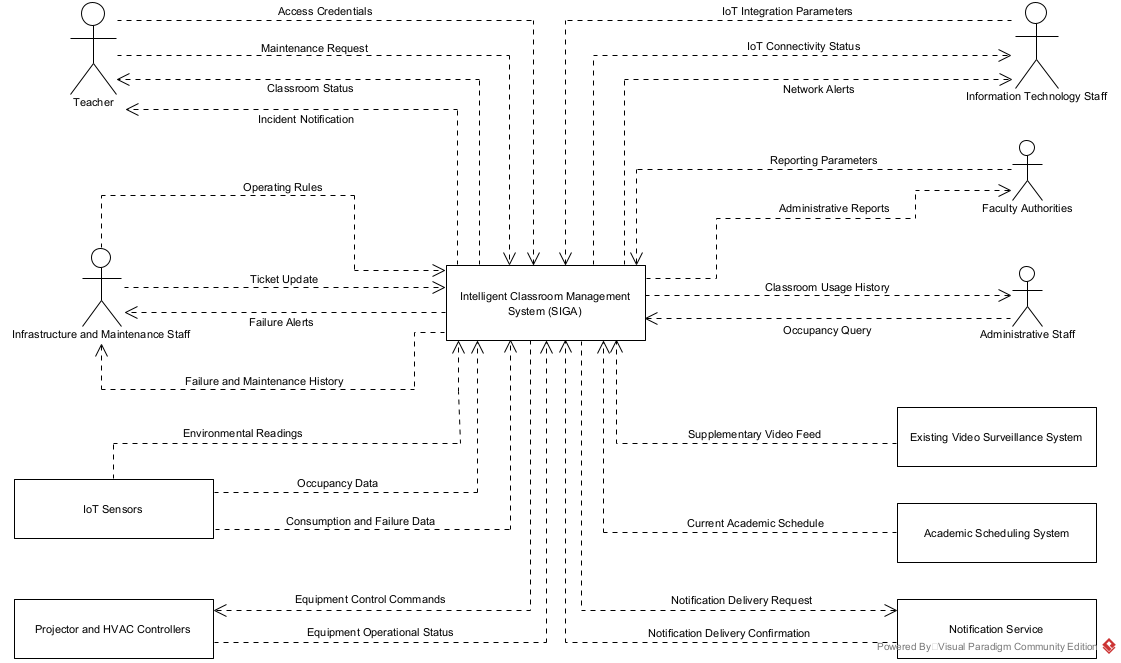
\includegraphics[width=0.85\textwidth,height=0.8\textheight,keepaspectratio]{figuras/System Context Diagram of the Intelligent Classroom Management System (SIGA).png}
\caption{Diagrama de contexto}
\label{fig:img1}
\end{figure}

Estudiantes y técnicos de mantenimiento externos no se modelan como actores directos del sistema en esta fase, ya que no requieren autenticación ni interacción directa con SIGA (ver Sección 2.3).


\subsection*{2.2 Funciones del producto}

\addcontentsline{toc}{subsection}{2.2 Funciones del producto}

\begin{itemize}\item Monitoreo y control remoto de sensores, proyectores y climatización.\end{itemize}

\begin{itemize}\item Detección automática de ocupación de aulas.\end{itemize}

\begin{itemize}\item Generación de alertas y mantenimiento predictivo mediante IA.\end{itemize}

\begin{itemize}\item Gestión energética: apagado automático y programación de horarios.\end{itemize}

\begin{itemize}\item Gestión de solicitudes de mantenimiento mediante tickets.\end{itemize}

\begin{itemize}\item Reportes y administración con acceso diferenciado por roles.\end{itemize}

\begin{itemize}\item Exportación y rectificación de datos personales del usuario, conforme a la LOPDP.\end{itemize}

\subsection*{2.3 Clases y características de usuarios}

\addcontentsline{toc}{subsection}{2.3 Clases y características de usuarios}

El Sistema Inteligente de Gestión de Aulas contará con distintos tipos de usuarios, definidos de acuerdo con sus responsabilidades dentro de la Facultad de Ciencias de la Computación y Diseño Digital. Cada perfil tendrá permisos diferenciados, con el propósito de garantizar que las funciones de monitoreo, control, mantenimiento, administración técnica y consulta de reportes sean utilizadas únicamente por usuarios autorizados.


\begingroup
\small
\begin{longtable}{|p{3.9cm}|p{3.9cm}|p{3.9cm}|p{3.9cm}|}
\hline
\cellcolor{sigagreen}\textcolor{white}{\textbf{Tipo de usuario}} & \cellcolor{sigagreen}\textcolor{white}{\textbf{Descripción del perfil}} & \cellcolor{sigagreen}\textcolor{white}{\textbf{Funciones principales}} & \cellcolor{sigagreen}\textcolor{white}{\textbf{Nivel de acceso}} \\ \hline
Administrador funcional / Personal de Infraestructura y Mantenimiento & Usuario responsable de supervisar el estado operativo de las aulas, equipos de climatización, proyectores y solicitudes de mantenimiento. & Monitorear aulas, recibir alertas de fallas, configurar reglas operativas, revisar historial de mantenimientos, actualizar tickets y validar el estado de los equipos. & Alto \\ \hline
Personal de Tecnologías de la Información (TI) & Usuario encargado de administrar la integración técnica del sistema, la conectividad de red, los dispositivos IoT y los mecanismos de seguridad asociados a la plataforma. & Configurar dispositivos IoT, revisar conectividad, administrar parámetros técnicos, supervisar alertas de red, gestionar accesos y apoyar la interoperabilidad con sistemas externos. & Alto \\ \hline
Docente & Usuario que utiliza las aulas durante el desarrollo de actividades académicas. & Consultar condiciones del aula, verificar el estado de proyectores o climatización, reportar fallas y dar seguimiento básico a solicitudes de mantenimiento. & Medio \\ \hline
Personal Administrativo & Usuario que requiere información sobre ocupación, uso de aulas y disponibilidad de recursos para apoyar la planificación institucional. & Consultar historial de uso de aulas, revisar reportes de ocupación, acceder a información administrativa y apoyar la gestión de espacios físicos. & Medio \\ \hline
Autoridades de la Facultad & Usuario directivo que requiere información consolidada para la toma de decisiones relacionadas con eficiencia energética, mantenimiento, inversión tecnológica y mejora de la infraestructura académica. & Consultar reportes administrativos, revisar indicadores de consumo energético, analizar estadísticas de uso y evaluar el estado general de la infraestructura. & Consulta estratégica \\ \hline
\caption{Características de usuarios y perfiles}
\end{longtable}
\endgroup

Los estudiantes se consideran beneficiarios indirectos del sistema. En esta fase no se contemplan como usuarios operativos de la plataforma, salvo en su rol de titulares de datos personales para efectos de las funciones RF-24 y RF-25 (Sección 3.2) derivadas del análisis normativo LOPDP.


\subsection*{2.4 Mapa de stakeholders}

\addcontentsline{toc}{subsection}{2.4 Mapa de stakeholders}

El Sistema Inteligente de Gestión de Aulas involucra a distintos stakeholders internos y externos de la Facultad de Ciencias de la Computación y Diseño Digital.


\begingroup
\small
\begin{longtable}{|p{2.6cm}|p{2.6cm}|p{2.6cm}|p{2.6cm}|p{2.6cm}|p{2.6cm}|}
\hline
\cellcolor{sigagreen}\textcolor{white}{\textbf{Stakeholder}} & \cellcolor{sigagreen}\textcolor{white}{\textbf{Interés en el sistema}} & \cellcolor{sigagreen}\textcolor{white}{\textbf{Poder}} & \cellcolor{sigagreen}\textcolor{white}{\textbf{Interés}} & \cellcolor{sigagreen}\textcolor{white}{\textbf{Necesidades y expectativas}} & \cellcolor{sigagreen}\textcolor{white}{\textbf{Estrategia de gestión}} \\ \hline
Autoridades de la Facultad & Mejorar la gestión de aulas, reducir costos operativos y disponer de información confiable para la toma de decisiones. & Alto & Alto & Reportes administrativos, indicadores de consumo energético, estado de equipos y datos de ocupación de aulas. & Gestionar de cerca mediante validación periódica de reportes, prioridades y criterios de eficiencia. \\ \hline
Departamento de Infraestructura y Mantenimiento & Supervisar el estado operativo de aulas, proyectores, climatización e incidencias técnicas. & Alto & Alto & Alertas tempranas, historial de fallas, solicitudes de mantenimiento y reducción de tiempos de respuesta. & Gestionar de cerca mediante coordinación directa de reglas operativas, atención de tickets y validación de alertas. \\ \hline
Personal de Tecnologías de la Información (TI) & Administrar la plataforma tecnológica, la conectividad, la integración IoT y la seguridad de datos. & Alto & Alto & Control de accesos, monitoreo de red, integración de sensores, interoperabilidad y protección de la información. & Gestionar de cerca mediante revisión técnica de arquitectura, permisos, conectividad y políticas de seguridad. \\ \hline
Docentes & Utilizar aulas funcionales durante el desarrollo de las clases. & Medio & Alto & Proyectores, climatización, conectividad y condiciones ambientales adecuadas para evitar interrupciones académicas. & Mantener informado y consultar mediante reportes de incidencias, encuestas o retroalimentación. \\ \hline
Estudiantes & Recibir clases en ambientes cómodos, seguros y tecnológicamente adecuados. & Bajo & Alto & Condiciones ambientales apropiadas, equipos operativos y menor interrupción de las actividades académicas. & Mantener informado de forma indirecta y considerar su percepción mediante cuestionarios de satisfacción. \\ \hline
Personal Administrativo & Consultar información relacionada con uso, ocupación y disponibilidad de aulas. & Medio & Medio & Reportes de ocupación, historial de uso y datos para apoyar la planificación de espacios académicos. & Mantener satisfecho mediante acceso a reportes claros y consultas administrativas. \\ \hline
Técnicos externos o proveedores & Atender reparaciones especializadas de equipos tecnológicos o sistemas de climatización. & Bajo & Bajo & Información precisa sobre fallas, ubicación del equipo afectado y antecedentes de mantenimiento. & Monitorear y coordinar únicamente cuando existan incidencias que requieran soporte especializado. \\ \hline
Universidad & Impulsar la modernización institucional, la eficiencia energética y la transformación digital del campus. & Alto & Alto & Reducción de costos, cumplimiento de políticas institucionales, mejora de infraestructura y sostenibilidad operativa. & Gestionar de cerca a nivel estratégico mediante informes consolidados y alineación con políticas institucionales. \\ \hline
\caption{Mapa de stakeholders}
\end{longtable}
\endgroup

\subsubsection*{2.4.1. Matriz poder/interés}

\addcontentsline{toc}{subsubsection}{2.4.1. Matriz poder/interés}

\begingroup
\small
\begin{longtable}{|p{3.1cm}|p{3.1cm}|p{3.1cm}|p{3.1cm}|p{3.1cm}|}
\hline
\cellcolor{sigagreen}\textcolor{white}{\textbf{Stakeholder}} & \cellcolor{sigagreen}\textcolor{white}{\textbf{Poder}} & \cellcolor{sigagreen}\textcolor{white}{\textbf{Interés}} & \cellcolor{sigagreen}\textcolor{white}{\textbf{Clasificación}} & \cellcolor{sigagreen}\textcolor{white}{\textbf{Estrategia}} \\ \hline
Autoridades de la Facultad & Alto & Alto & Actor clave & Gestionar de cerca \\ \hline
Departamento de Infraestructura y Mantenimiento & Alto & Alto & Actor clave & Gestionar de cerca \\ \hline
Personal de Tecnologías de la Información (TI) & Alto & Alto & Actor clave & Gestionar de cerca \\ \hline
Docentes & Medio & Alto & Mantener informado & Mantener informado \\ \hline
Estudiantes & Bajo & Alto & Mantener informado & Mantener informado \\ \hline
Personal Administrativo & Medio & Medio & Mantener satisfecho & Monitorear \\ \hline
Técnicos externos o proveedores & Bajo & Bajo & Esfuerzo mínimo & Monitorear \\ \hline
Universidad & Alto & Alto & Actor clave & Gestionar de cerca \\ \hline
\caption{Matriz poder/interés}
\end{longtable}
\endgroup

\subsubsection*{2.4.2. Conflictos potenciales entre stakeholders}

\addcontentsline{toc}{subsubsection}{2.4.2. Conflictos potenciales entre stakeholders}

\begingroup
\small
\begin{longtable}{|p{3.1cm}|p{3.1cm}|p{3.1cm}|p{3.1cm}|p{3.1cm}|}
\hline
\cellcolor{sigagreen}\textcolor{white}{\textbf{Conflicto potencial}} & \cellcolor{sigagreen}\textcolor{white}{\textbf{Stakeholders involucrados}} & \cellcolor{sigagreen}\textcolor{white}{\textbf{Causa del conflicto}} & \cellcolor{sigagreen}\textcolor{white}{\textbf{Impacto posible en el sistema}} & \cellcolor{sigagreen}\textcolor{white}{\textbf{Estrategia de gestión}} \\ \hline
Ahorro energético frente a confort térmico & Autoridades, Universidad, Docentes, Estudiantes, Infraestructura & Las autoridades pueden priorizar la reducción del consumo energético, mientras que docentes y estudiantes requieren condiciones ambientales adecuadas. & Configuración inadecuada de reglas automáticas de climatización o reducción del confort en las aulas. & Definir parámetros mínimos y máximos de temperatura, validar reglas con Infraestructura y recoger retroalimentación. \\ \hline
Seguridad tecnológica frente a facilidad de integración IoT & Personal de TI, Infraestructura y Mantenimiento & TI puede exigir controles de seguridad, mientras que Infraestructura requiere una integración rápida de sensores. & Retrasos en la instalación de dispositivos IoT o incompatibilidad con equipos existentes. & Establecer criterios técnicos de integración, protocolos permitidos y validaciones de seguridad antes del despliegue. \\ \hline
Control remoto de equipos frente a responsabilidad operativa & Docentes, Infraestructura, TI & Los docentes pueden requerir disponibilidad inmediata de proyectores, mientras Mantenimiento conserva el control sobre reglas de apagado. & Acciones contradictorias sobre los equipos o fallas por configuración incorrecta. & Definir roles y permisos diferenciados, registrar acciones en bitácora y limitar el control remoto a usuarios autorizados. \\ \hline
Uso de videovigilancia frente a privacidad institucional & Autoridades, TI, Docentes, Estudiantes & La integración con cámaras puede generar preocupación sobre privacidad o acceso no autorizado al flujo de video. & Rechazo de usuarios o incumplimiento de políticas de protección de datos. & Usar las cámaras solo como fuente complementaria, restringir accesos y documentar el uso permitido. \\ \hline
Priorización de mantenimiento frente a disponibilidad presupuestaria & Infraestructura, Autoridades, Universidad, Proveedores externos & El sistema puede detectar fallas recurrentes, pero la atención dependerá de recursos económicos y personal disponible. & Acumulación de tickets, demoras en reparaciones o pérdida de confianza en las alertas. & Clasificar incidencias por criticidad, justificar prioridades con evidencia histórica y generar reportes presupuestarios. \\ \hline
Automatización de apagado frente a continuidad académica & Docentes, Estudiantes, Infraestructura, Administrativo & Las reglas automáticas pueden apagar equipos cuando el aula se detecte desocupada, aunque existan clases extendidas. & Interrupción de clases, apagado indebido de climatización o proyectores. & Integrar el horario académico vigente, permitir excepciones autorizadas y registrar actividades extraordinarias. \\ \hline
Reportes administrativos frente a calidad de datos recolectados & Autoridades, Administrativo, TI, Sensores IoT & Los reportes dependen de datos correctos; si los sensores fallan, la información puede ser incompleta. & Decisiones administrativas basadas en datos incorrectos o pérdida de confiabilidad del sistema. & Implementar validaciones de datos, monitoreo de conectividad y revisión periódica de consistencia. \\ \hline
Expectativas institucionales frente al alcance real de la fase & Universidad, Autoridades, TI, Infraestructura & Algunos stakeholders pueden esperar que el sistema controle todos los recursos del campus. & Sobrecarga de requisitos, ampliación no controlada del alcance o retrasos en la entrega. & Mantener documentado el alcance del producto y evaluar ampliaciones en fases posteriores. \\ \hline
\caption{Conflictos potenciales entre stakeholders}
\end{longtable}
\endgroup

\subsection*{2.5 Entorno operativo}

\addcontentsline{toc}{subsection}{2.5 Entorno operativo}

El Sistema Inteligente de Gestión de Aulas operará en un entorno institucional compuesto por aulas, laboratorios, dispositivos IoT, red de datos de la facultad y una plataforma web centralizada.


\begingroup
\small
\begin{longtable}{|p{7.8cm}|p{7.8cm}|}
\hline
\cellcolor{sigagreen}\textcolor{white}{\textbf{Componente de hardware}} & \cellcolor{sigagreen}\textcolor{white}{\textbf{Descripción operativa}} \\ \hline
Sensores de temperatura y humedad & Capturan las condiciones ambientales del aula para su monitoreo en tiempo real. \\ \hline
Sensores de presencia u ocupación & Permiten identificar si el aula se encuentra ocupada o desocupada. \\ \hline
Sensores o módulos de consumo energético & Registran datos relacionados con el consumo de equipos, cuando la infraestructura lo permita. \\ \hline
Controladores de proyector & Permiten consultar el estado operativo del proyector y ejecutar comandos compatibles de control remoto. \\ \hline
Controladores de climatización & Permiten monitorear o ajustar el funcionamiento de equipos de aire acondicionado compatibles. \\ \hline
Gateway IoT & Consolida los datos generados por sensores y dispositivos embebidos para enviarlos a la plataforma central. \\ \hline
Cámaras de videovigilancia existentes & Se consideran como fuente complementaria de monitoreo visual, sin reemplazar el sistema de videovigilancia actual. \\ \hline
Servidor o servicio de alojamiento & Ejecuta la plataforma web, almacena información y gestiona la comunicación con los dispositivos IoT. \\ \hline
\caption{Componentes de hardware y descripción operativa}
\end{longtable}
\endgroup

\begingroup
\small
\begin{longtable}{|p{7.8cm}|p{7.8cm}|}
\hline
\cellcolor{sigagreen}\textcolor{white}{\textbf{Componente de software}} & \cellcolor{sigagreen}\textcolor{white}{\textbf{Descripción operativa}} \\ \hline
Plataforma web del sistema & Permite el monitoreo de aulas, control remoto de equipos, gestión de alertas, solicitudes de mantenimiento y reportes. \\ \hline
Sistema operativo del servidor & Podrá ejecutarse sobre un entorno servidor Linux o Windows Server, según la infraestructura disponible. \\ \hline
Base de datos & Almacena datos de sensores, usuarios, roles, aulas, equipos, alertas, mantenimientos, reportes y bitácoras. \\ \hline
Navegadores soportados & La interfaz deberá funcionar en Google Chrome, Mozilla Firefox y Microsoft Edge. \\ \hline
API REST & Permitirá la comunicación entre la plataforma, servicios externos y módulos de integración. \\ \hline
Servicio de notificaciones & Gestionará el envío de alertas por correo electrónico, aplicación móvil u otro canal institucional. \\ \hline
Módulo de análisis de datos & Procesará históricos de consumo, ocupación y fallas para apoyar el mantenimiento preventivo. \\ \hline
\caption{Componentes de hardware y descripción operativa}
\end{longtable}
\endgroup

\begingroup
\small
\begin{longtable}{|p{7.8cm}|p{7.8cm}|}
\hline
\cellcolor{sigagreen}\textcolor{white}{\textbf{Elemento de red}} & \cellcolor{sigagreen}\textcolor{white}{\textbf{Descripción operativa}} \\ \hline
Red Wi-Fi institucional & Permitirá la conexión de sensores, gateways o dispositivos embebidos ubicados en las aulas. \\ \hline
Red cableada institucional & Podrá utilizarse para equipos fijos, gateways, cámaras o servidores que requieran mayor estabilidad. \\ \hline
Protocolos de comunicación & Se considerarán protocolos compatibles con IoT, como MQTT, HTTP o mecanismos basados en API REST. \\ \hline
Seguridad de red & La comunicación deberá operar bajo controles de acceso, autenticación y segmentación definidos por TI. \\ \hline
Disponibilidad de conectividad & El monitoreo en tiempo real dependerá de una conexión estable entre dispositivos IoT, gateways y plataforma. \\ \hline
\caption{Componentes de software y descripción operativa}
\end{longtable}
\endgroup

\subsection*{2.6 Suposiciones y dependencias}

\addcontentsline{toc}{subsection}{2.6 Suposiciones y dependencias}

\subsubsection*{2.6.1. Suposiciones}

\addcontentsline{toc}{subsubsection}{2.6.1. Suposiciones}

\begingroup
\small
\begin{longtable}{|p{5.2cm}|p{5.2cm}|p{5.2cm}|}
\hline
\cellcolor{sigagreen}\textcolor{white}{\textbf{ID}} & \cellcolor{sigagreen}\textcolor{white}{\textbf{Suposición}} & \cellcolor{sigagreen}\textcolor{white}{\textbf{Descripción}} \\ \hline
SUP-01 & Disponibilidad de conectividad en las aulas & Se asume que las aulas y laboratorios contarán con conectividad Wi-Fi o red cableada estable. \\ \hline
SUP-02 & Compatibilidad técnica de los equipos & Se asume que los proyectores y sistemas de climatización podrán integrarse con controladores compatibles. \\ \hline
SUP-03 & Acceso autorizado a la infraestructura física & Se asume que Infraestructura y Mantenimiento permitirá el acceso para instalación y validación de dispositivos. \\ \hline
SUP-04 & Participación de usuarios clave & Se asume que Infraestructura, TI, docentes y autoridades colaborarán en validación, entrevistas y pruebas. \\ \hline
SUP-05 & Uso institucional de la plataforma & Se asume que los usuarios autorizados utilizarán la plataforma conforme a los roles asignados. \\ \hline
SUP-06 & Disponibilidad de información histórica & Se asume que se almacenarán datos suficientes para aplicar análisis mediante IA. \\ \hline
SUP-07 & Condiciones de operación normales & Se asume que los dispositivos IoT operarán en condiciones ambientales propias de aulas y laboratorios. \\ \hline
\caption{Suposiciones}
\end{longtable}
\endgroup

\subsubsection*{2.6.2. Dependencias}

\addcontentsline{toc}{subsubsection}{2.6.2. Dependencias}

\begingroup
\small
\begin{longtable}{|p{5.2cm}|p{5.2cm}|p{5.2cm}|}
\hline
\cellcolor{sigagreen}\textcolor{white}{\textbf{ID}} & \cellcolor{sigagreen}\textcolor{white}{\textbf{Dependencia}} & \cellcolor{sigagreen}\textcolor{white}{\textbf{Descripción}} \\ \hline
DEP-01 & Red institucional & El sistema depende de la disponibilidad y estabilidad de la red institucional. \\ \hline
DEP-02 & Horario académico vigente & El sistema depende del horario académico en formato digital o estructurado. \\ \hline
DEP-03 & Personal de TI & El sistema depende del personal de TI para validar integración, red, accesos y seguridad. \\ \hline
DEP-04 & Departamento de Infraestructura y Mantenimiento & El sistema depende de este departamento para instalar sensores, validar alertas y atender tickets. \\ \hline
DEP-05 & Equipos compatibles & El sistema depende de proyectores y climatizadores compatibles con monitoreo o control remoto. \\ \hline
DEP-06 & Sistema de videovigilancia existente & La integración con cámaras dependerá de disponibilidad técnica y permisos institucionales. \\ \hline
DEP-07 & Servicios de notificación & El envío de alertas dependerá de servicios institucionales o externos de notificación. \\ \hline
DEP-08 & Políticas institucionales de seguridad y privacidad & El sistema dependerá de las políticas definidas por la institución (LOPDP). \\ \hline
DEP-09 & Suministro eléctrico & El funcionamiento de sensores, gateways y plataforma dependerá del suministro eléctrico. \\ \hline
\caption{Dependencias}
\end{longtable}
\endgroup

\subsection*{2.7 Modelado organizacional i* - Diagramas SD y SR}

\addcontentsline{toc}{subsection}{2.7 Modelado organizacional i* - Diagramas SD y SR}

Nuevo en esta entrega. El lenguaje i* (distributed intentionality, Yu, 1995) modela la intencionalidad de los actores organizacionales mediante dos vistas complementarias: el Diagrama de Dependencia Estratégica (SD) y el Diagrama de Razón Estratégica (SR).


Diagrama de Dependencia Estratégica (SD) --- elaborado en draw.io (https://www.drawio.com/), con etiquetas en inglés conforme a lo indicado por el docente responsable: el actor ``Docente'' depende del actor ``Personal de Infraestructura y Mantenimiento'' para obtener ``clima y equipos operativos''; ``Personal de Infraestructura y Mantenimiento'' depende de ``SIGA'' para el recurso ``datos de sensores en tiempo real''; ``Autoridades de la Facultad'' dependen de ``SIGA'' para el softgoal ``reducir consumo energético''; ``Personal de TI'' depende de ``SIGA'' para la tarea ``gestionar accesos y roles''.


Diagrama de Razón Estratégica (SR) para el actor ``Personal de Infraestructura y Mantenimiento'' --- elaborado en draw.io: el softgoal ``reducir tiempo de respuesta a fallas'' se descompone en las tareas ``consultar panel de control'' (RF-07), ``recibir alertas automáticas'' (RF-08) y ``registrar mantenimiento'' (RF-12), cada una soportada por un RF del sistema SIGA.


\begin{figure}[H]
\centering
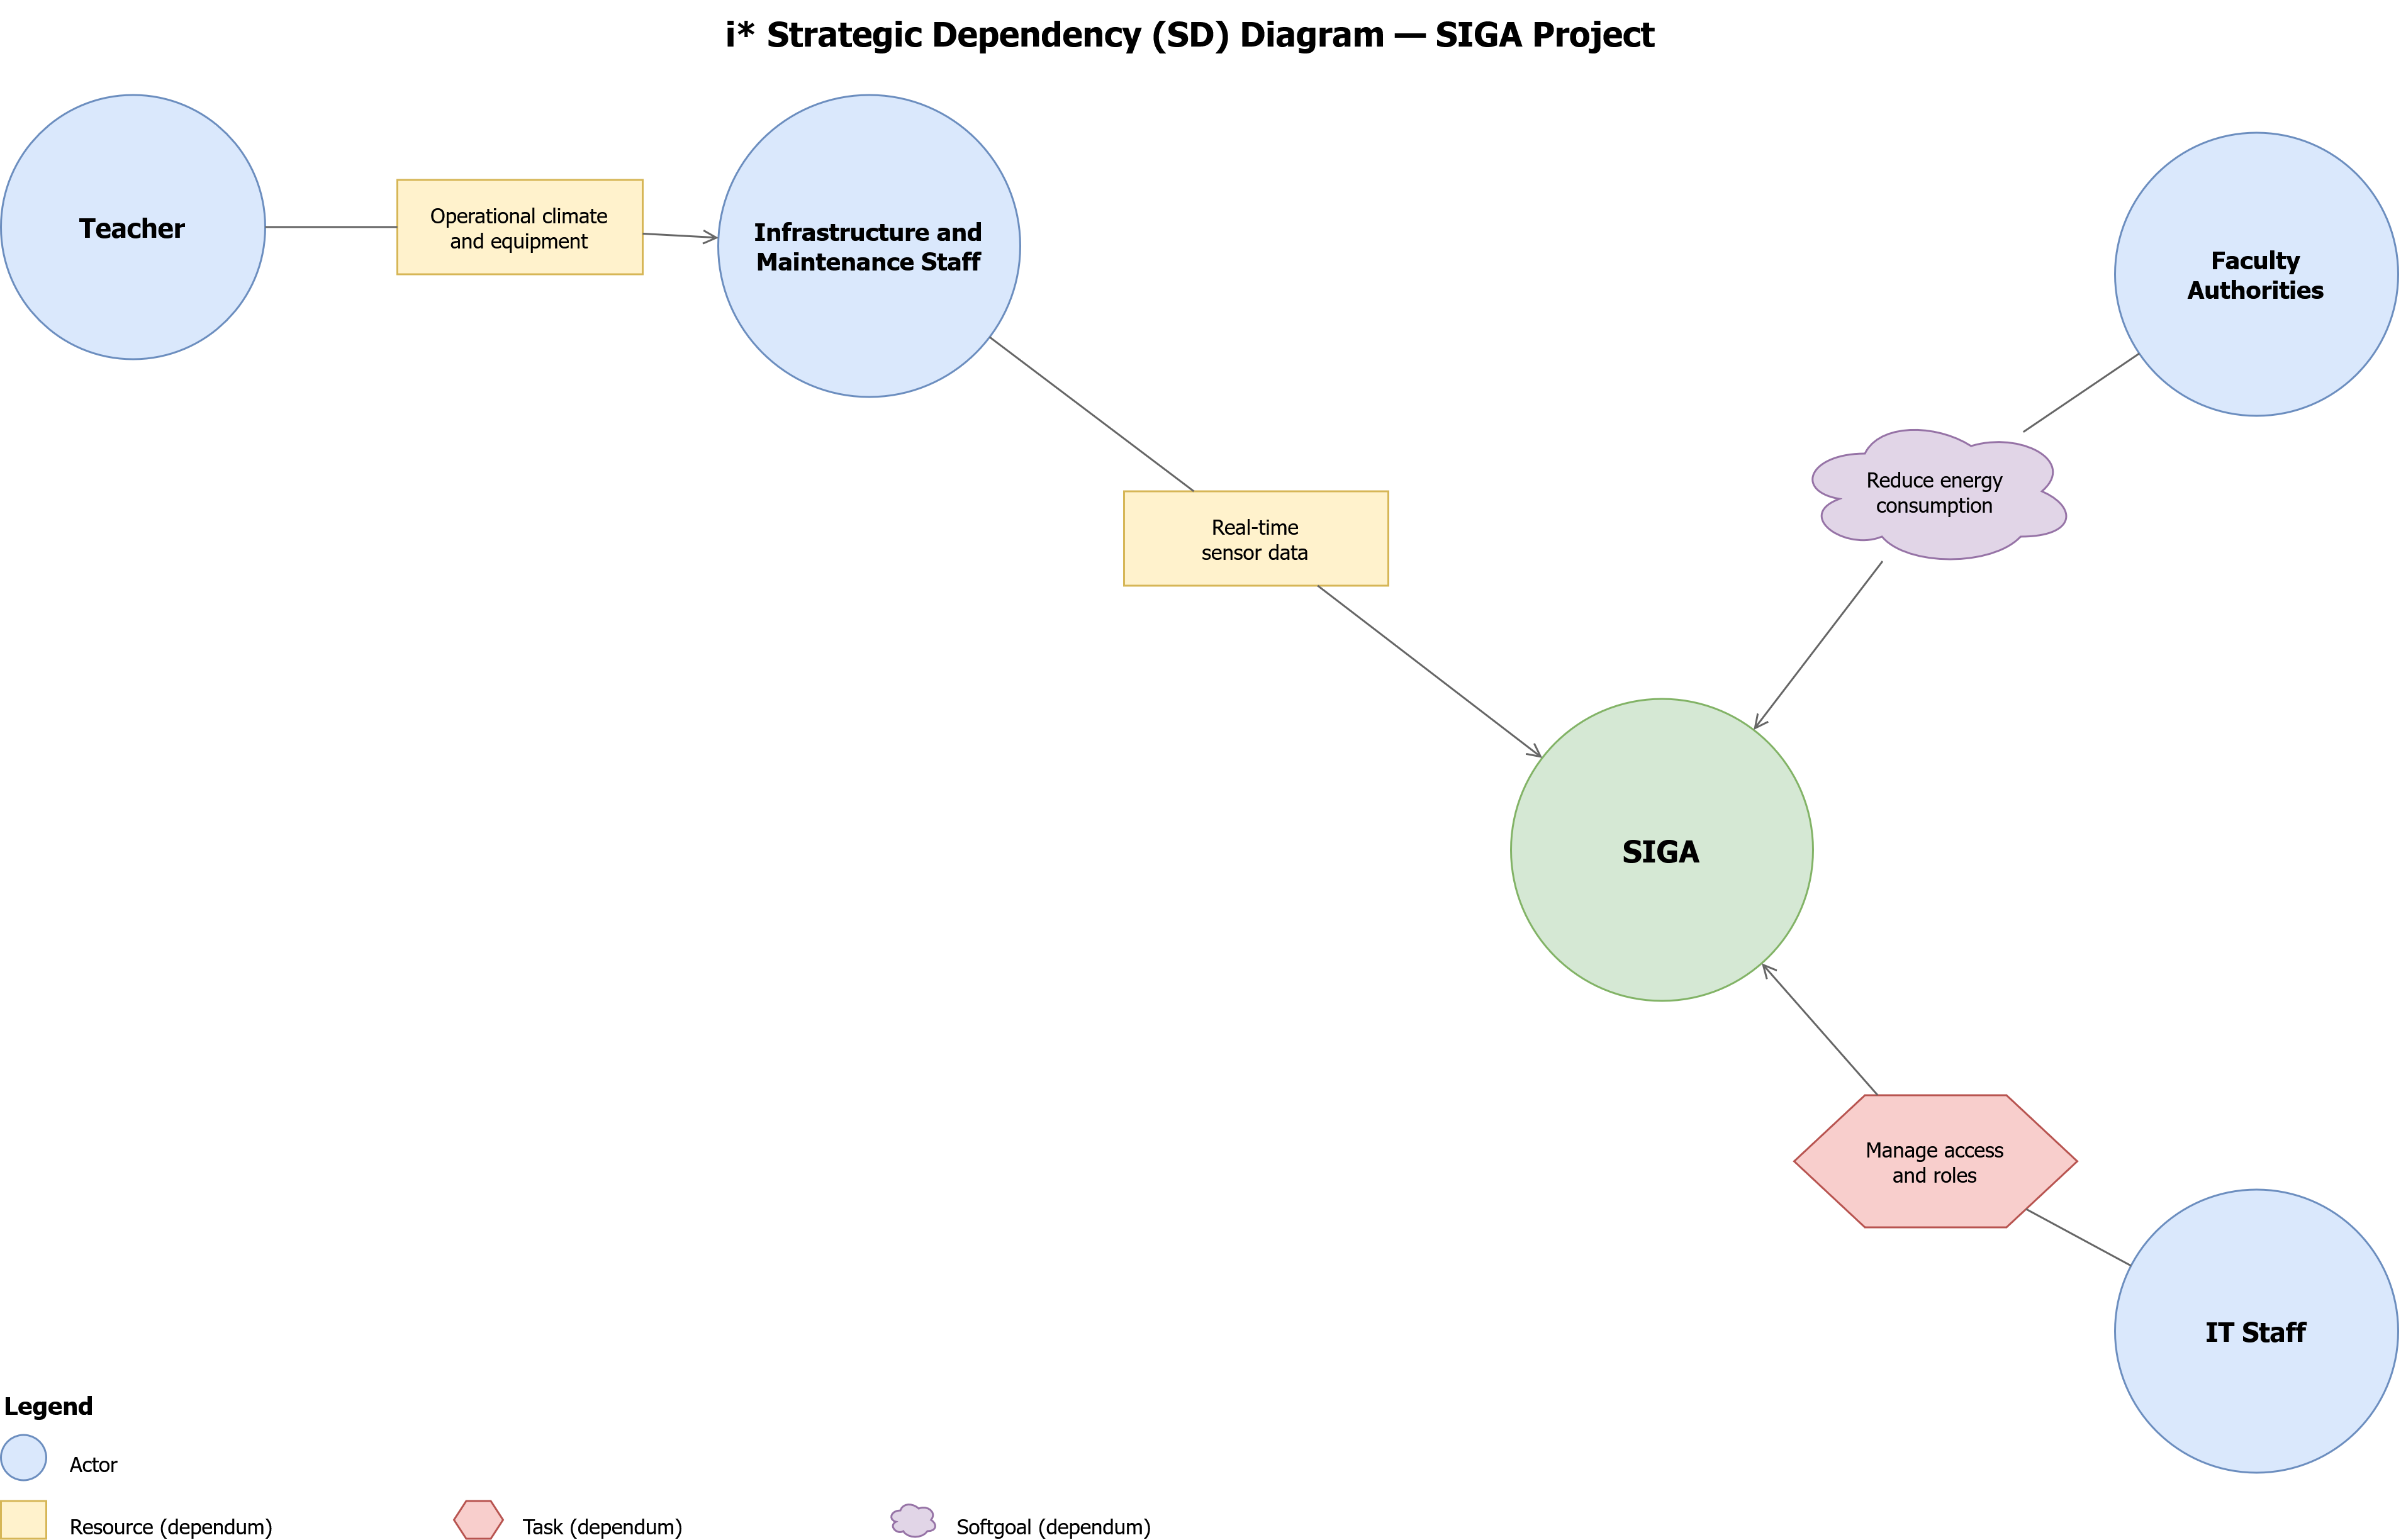
\includegraphics[width=0.85\textwidth,height=0.8\textheight,keepaspectratio]{figuras/istar_SD.drawio.png}
\caption{Diagrama i* de Dependencia Estratégica (SD)}
\label{fig:img2}
\end{figure}

\begin{figure}[H]
\centering
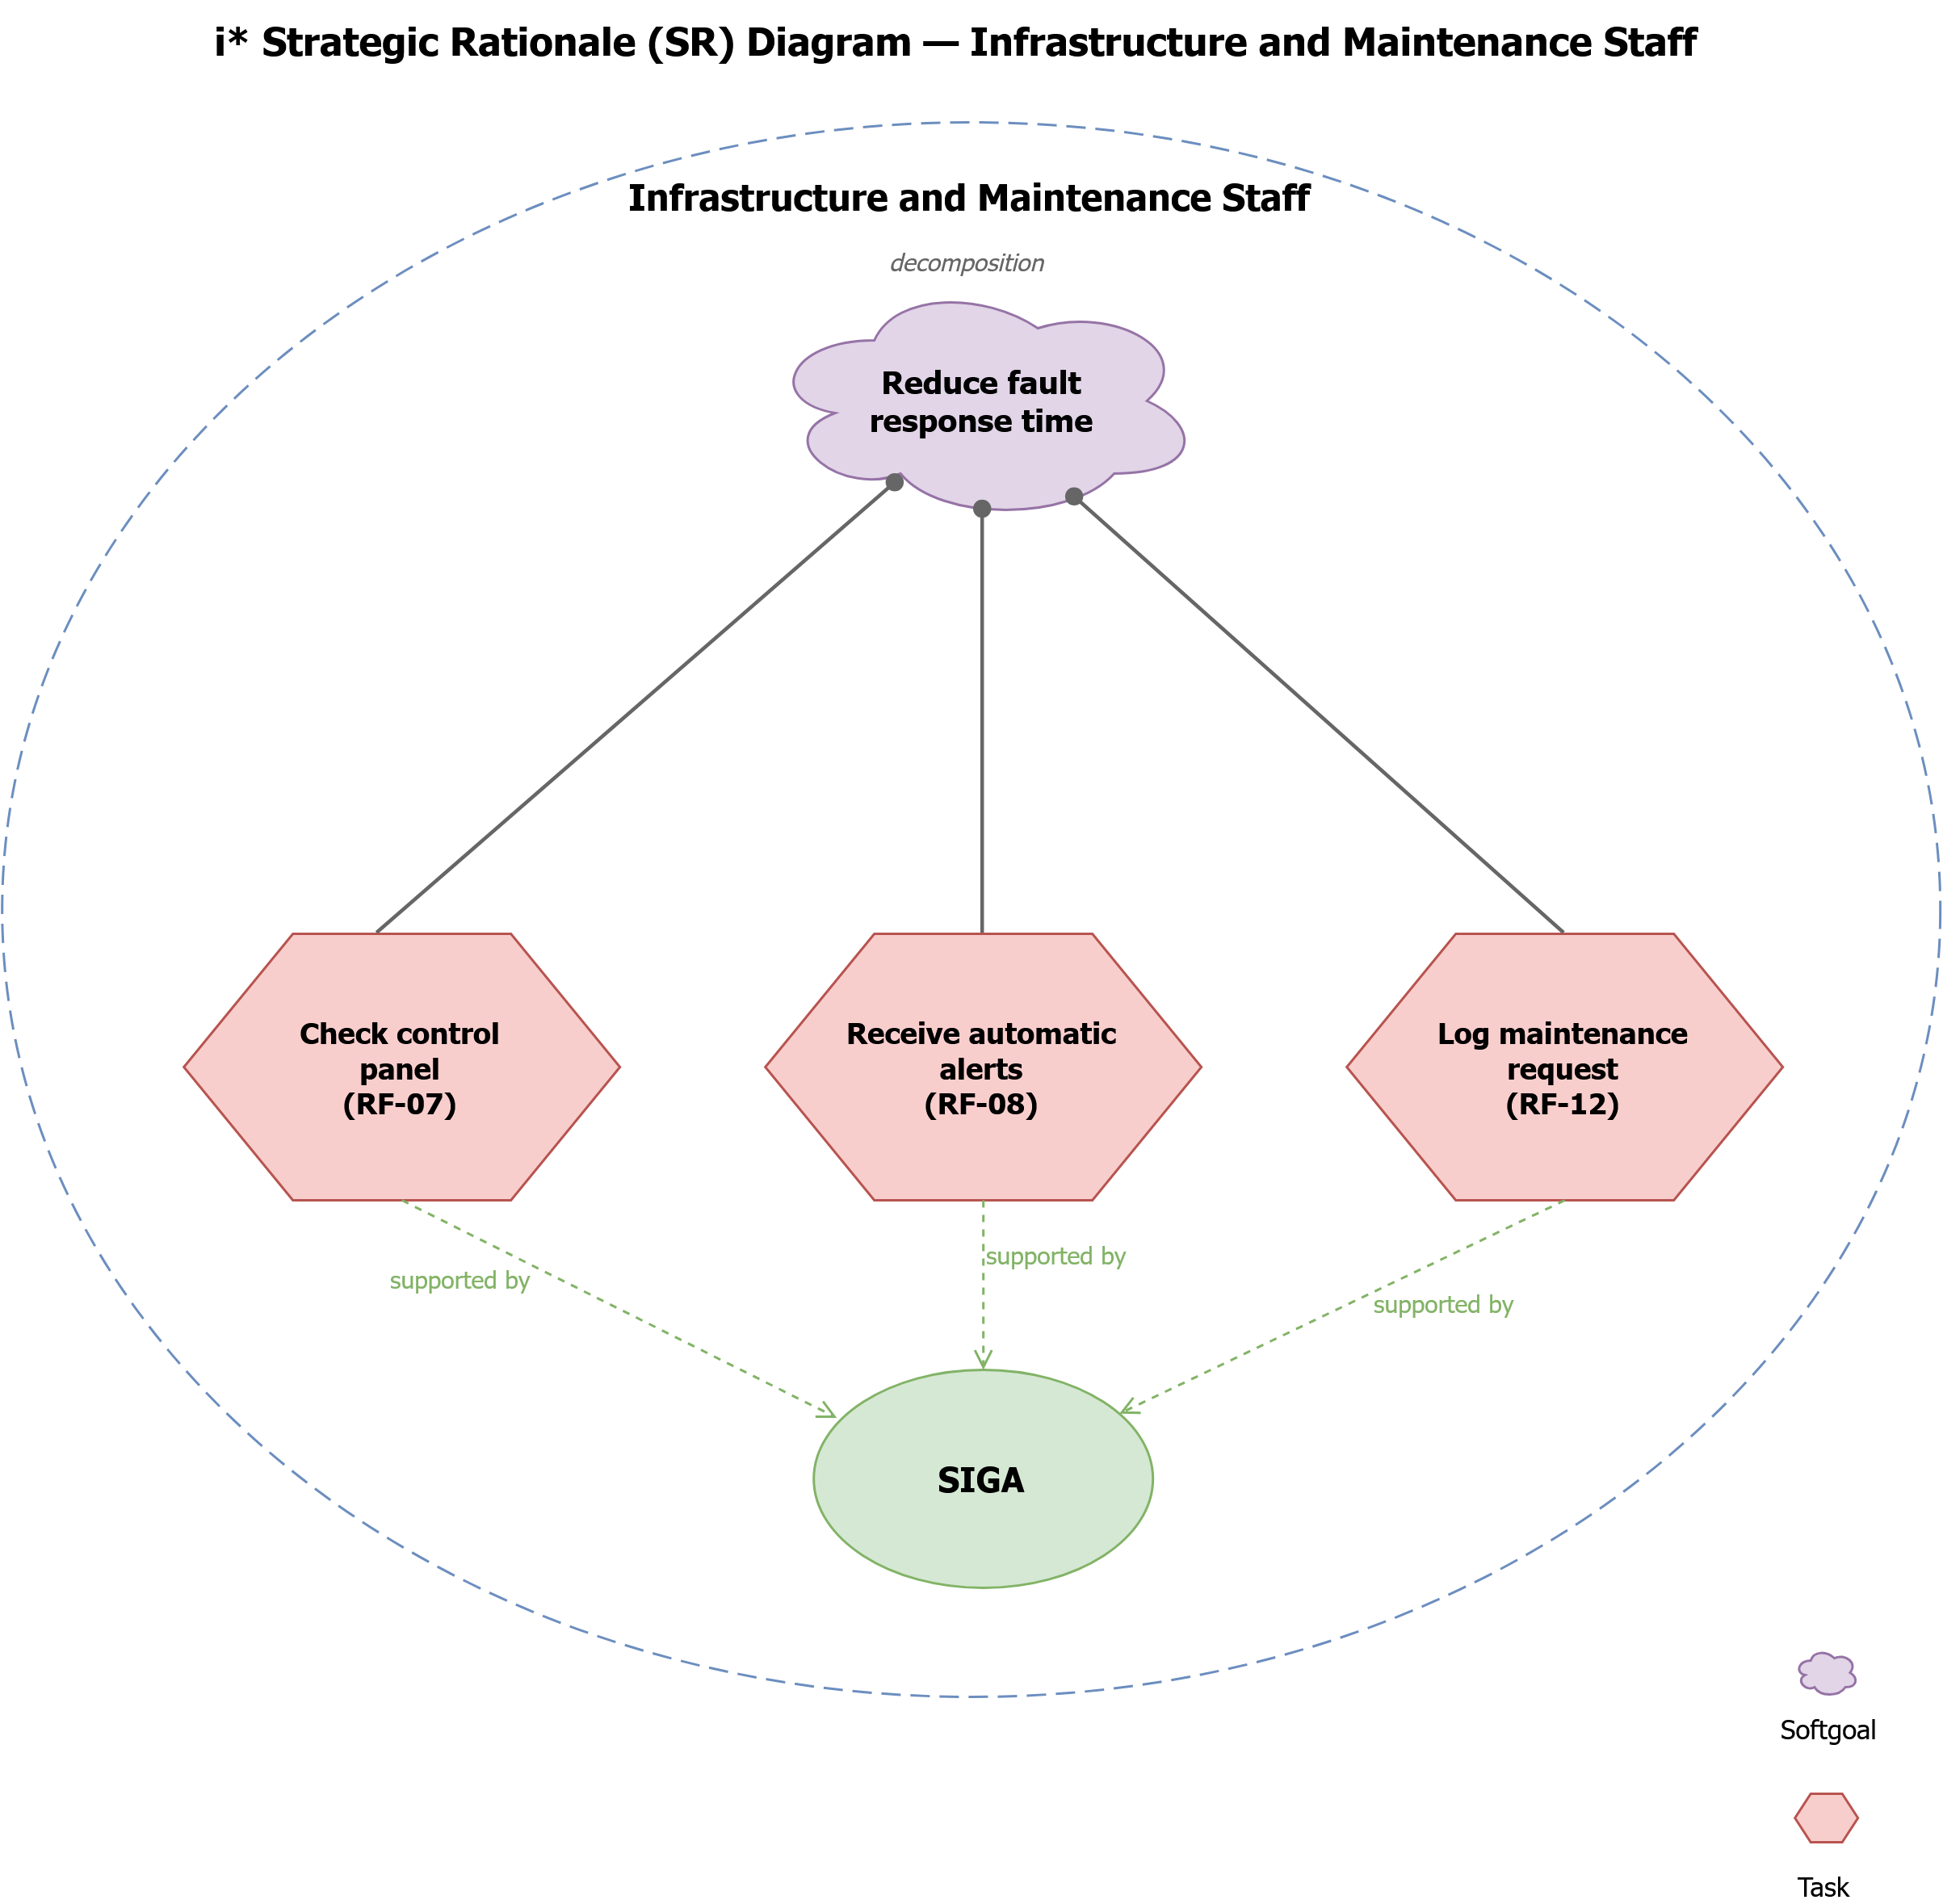
\includegraphics[width=0.85\textwidth,height=0.8\textheight,keepaspectratio]{figuras/iStar_SR.drawio.png}
\caption{Diagrama i* de Razón Estratégica (SR) --- Departamento de Infraestructura y Mantenimiento}
\label{fig:img3}
\end{figure}

\section*{III. REQUISITOS ESPECÍFICOS COMPLETOS}

\addcontentsline{toc}{section}{III. REQUISITOS ESPECÍFICOS COMPLETOS}

\subsection*{3.1 Interfaces externas (usuario, hardware, software) con mockups}

\addcontentsline{toc}{subsection}{3.1 Interfaces externas (usuario, hardware, software) con mockups}

Esta sección describe las interfaces externas del Sistema Inteligente de Gestión de Aulas, considerando la interacción con usuarios, dispositivos físicos, sensores IoT, controladores, sistemas externos y servicios de software.


\subsubsection*{3.1.1 Interfaces de usuario}

\addcontentsline{toc}{subsubsection}{3.1.1 Interfaces de usuario}

La plataforma contará con una interfaz web accesible desde navegadores modernos. Los mockups elaborados representan las principales pantallas del sistema.


\begin{figure}[H]
\centering
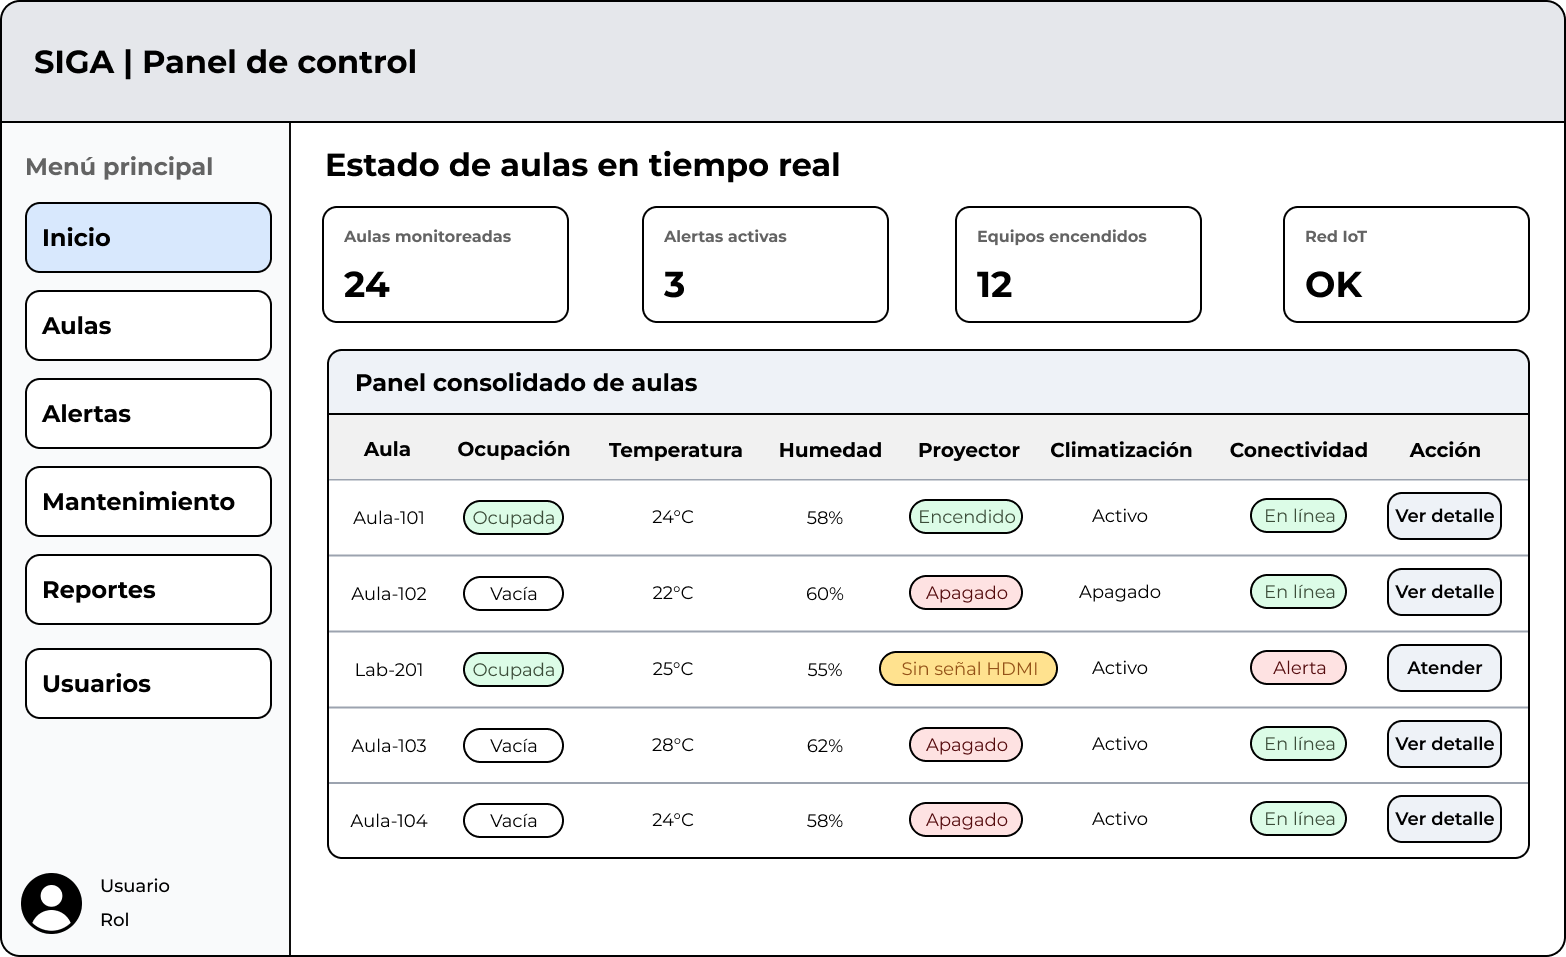
\includegraphics[width=0.85\textwidth,height=0.8\textheight,keepaspectratio]{figuras/Mockups SIGA - Panel.png}
\caption{Mockup MU-01: Panel de control centralizado}
\label{fig:img4}
\end{figure}

El panel de control centralizado permitirá visualizar el estado general de las aulas en tiempo real: ocupación, temperatura, humedad, estado del proyector, climatización, conectividad IoT y alertas activas.


\begin{figure}[H]
\centering
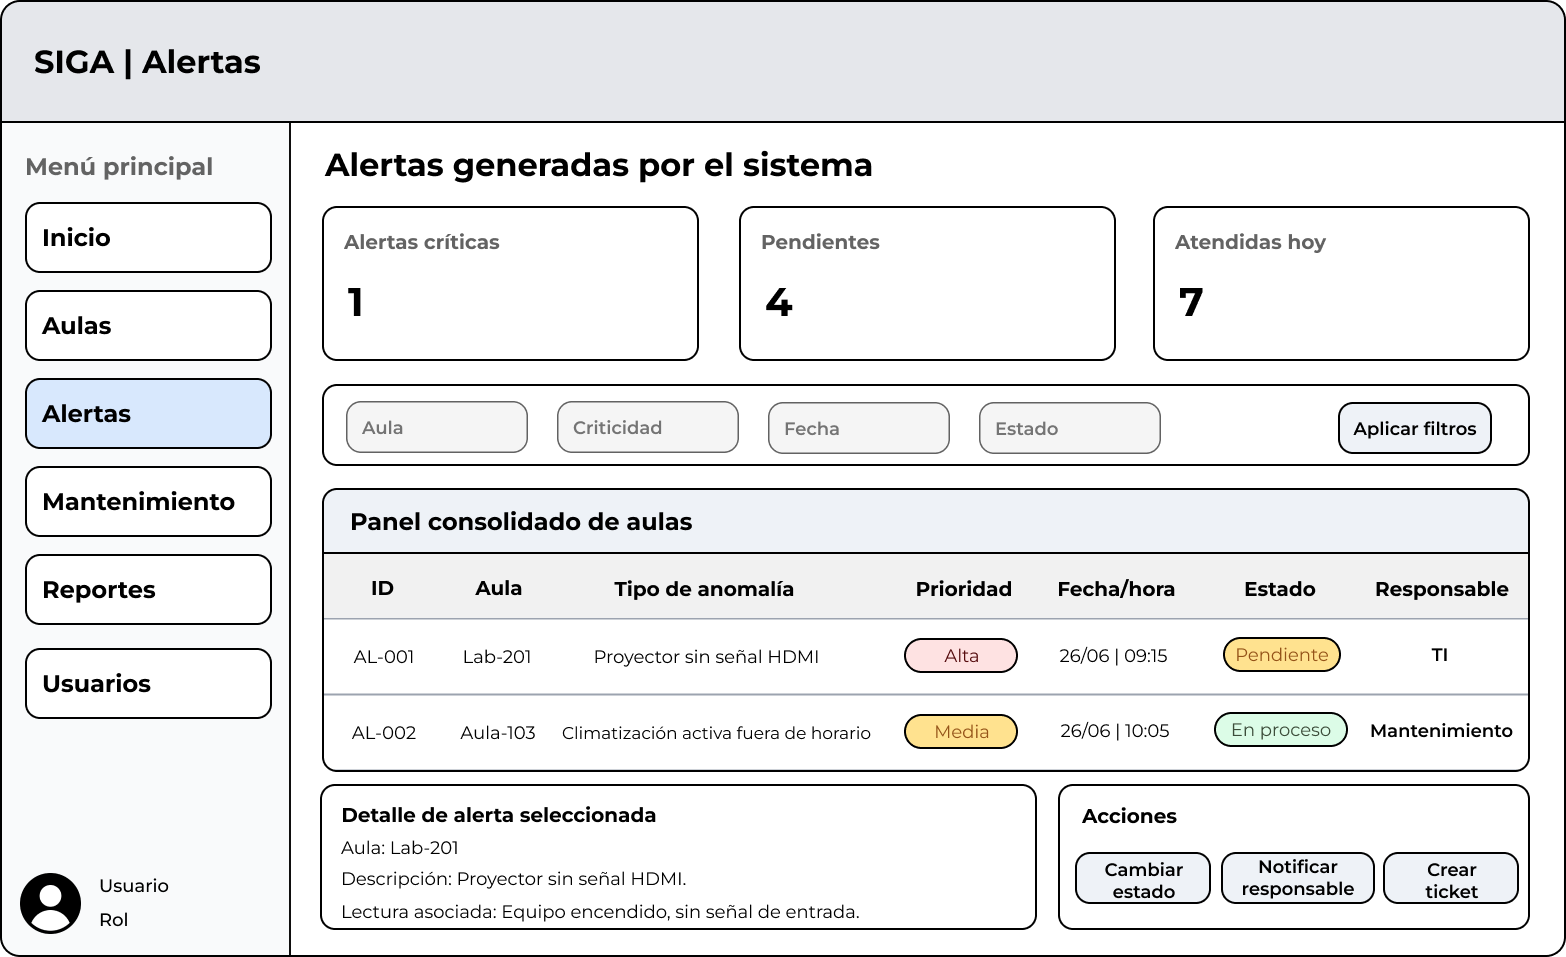
\includegraphics[width=0.85\textwidth,height=0.8\textheight,keepaspectratio]{figuras/Mockups SIGA - Alertas.png}
\caption{Mockup MU-02: Vista de alertas}
\label{fig:img5}
\end{figure}

La vista de alertas permitirá consultar identificador, aula afectada, tipo de anomalía, prioridad, fecha, hora, estado de atención y responsable asignado.


\begin{figure}[H]
\centering
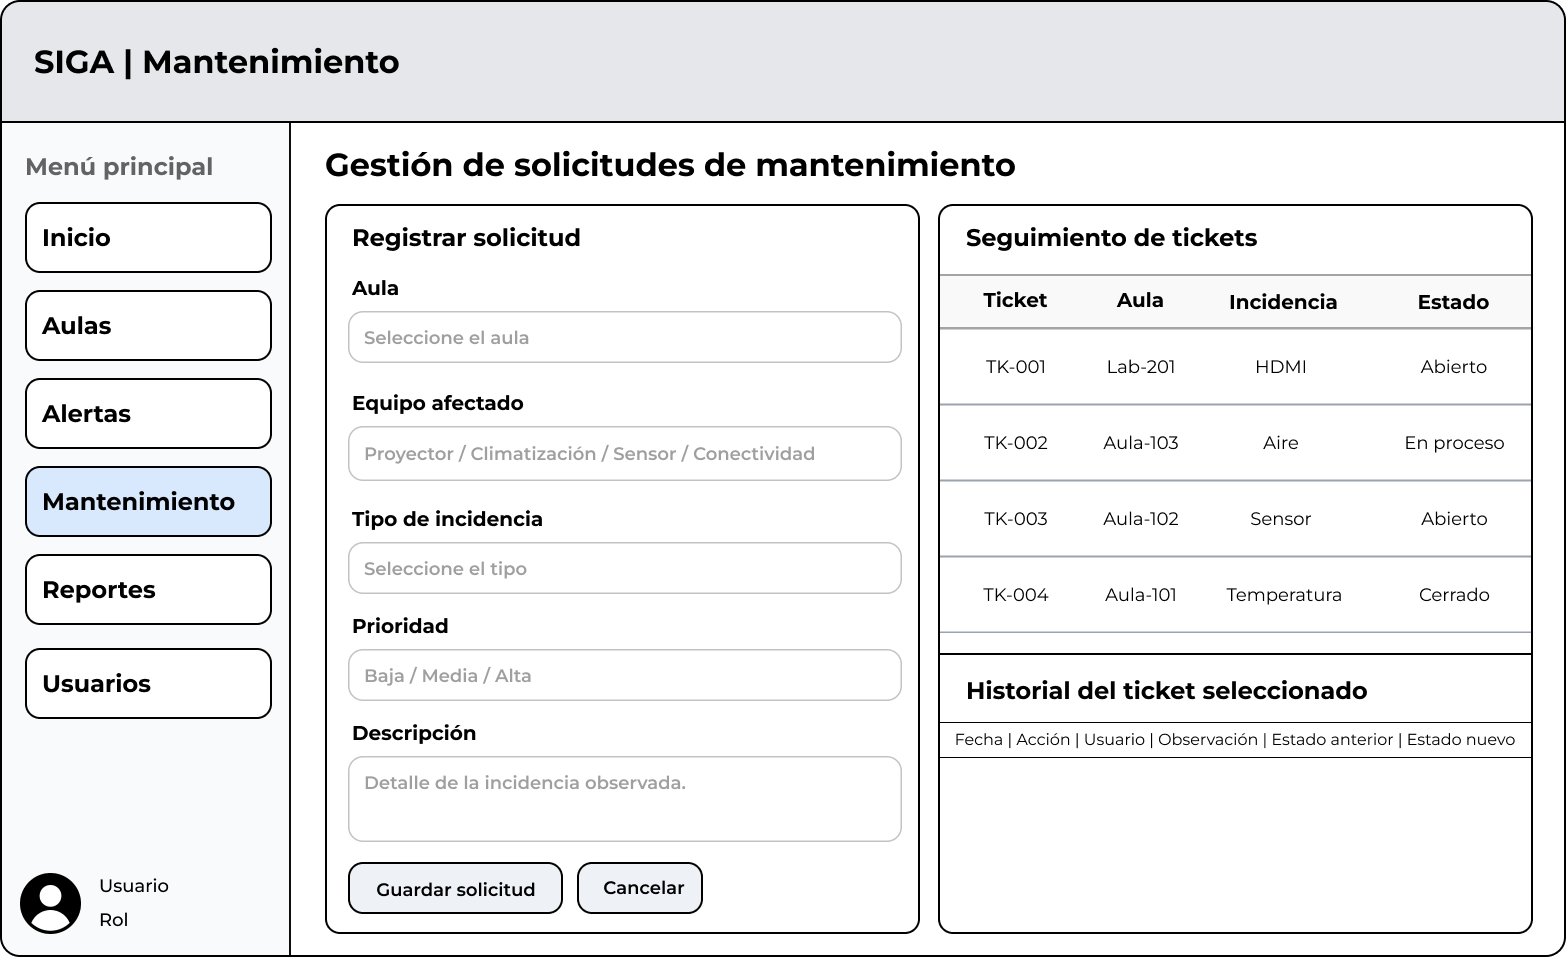
\includegraphics[width=0.85\textwidth,height=0.8\textheight,keepaspectratio]{figuras/Mockups SIGA - Mantenimiento.png}
\caption{Mockup MU-03: Módulo de mantenimiento}
\label{fig:img6}
\end{figure}

El módulo de mantenimiento permitirá registrar solicitudes y dar seguimiento a tickets: aula, equipo, tipo de incidencia, prioridad, descripción y estado.


\begin{figure}[H]
\centering
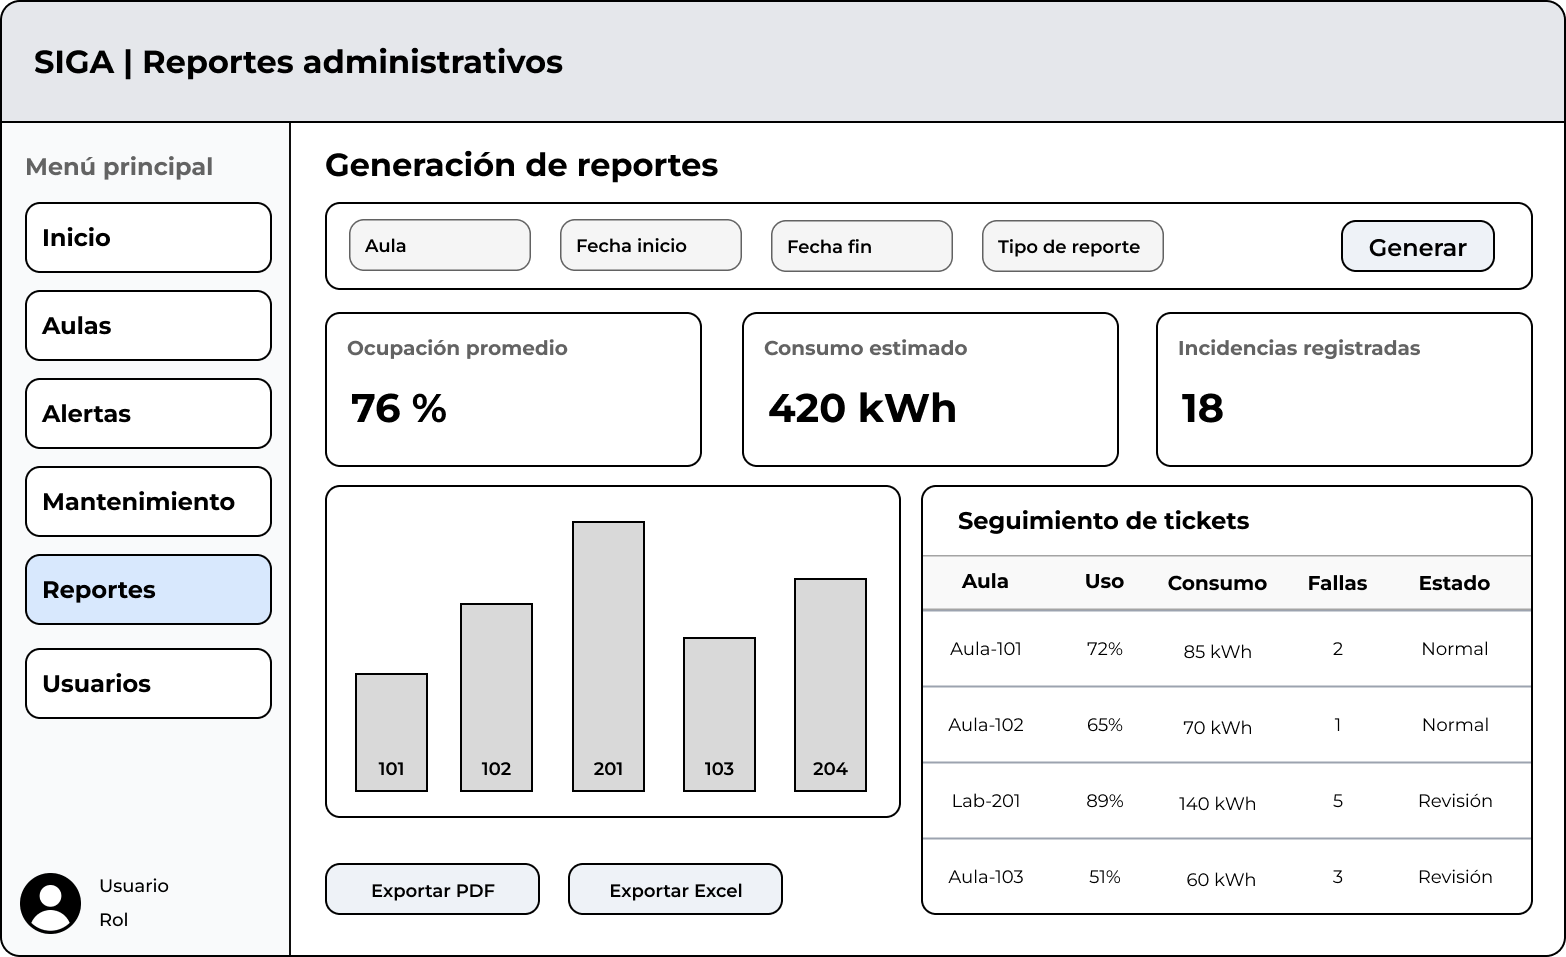
\includegraphics[width=0.85\textwidth,height=0.8\textheight,keepaspectratio]{figuras/Mockups SIGA - Reportes.png}
\caption{Mockup MU-04: Reportes administrativos}
\label{fig:img7}
\end{figure}

La vista de reportes administrativos permitirá consultar uso de aulas, ocupación, consumo energético, fallas y estado de equipos, con opciones de exportación.


\begingroup
\small
\begin{longtable}{|p{3.1cm}|p{3.1cm}|p{3.1cm}|p{3.1cm}|p{3.1cm}|}
\hline
\cellcolor{sigagreen}\textcolor{white}{\textbf{ID mockup}} & \cellcolor{sigagreen}\textcolor{white}{\textbf{Pantalla}} & \cellcolor{sigagreen}\textcolor{white}{\textbf{Usuario principal}} & \cellcolor{sigagreen}\textcolor{white}{\textbf{RF vinculados}} & \cellcolor{sigagreen}\textcolor{white}{\textbf{Justificación}} \\ \hline
MU-01 & Panel de control centralizado & Infraestructura, TI, Autoridades & RF-01, RF-03, RF-04, RF-05, RF-07 & Consolida lecturas ambientales, ocupación y estado operativo de equipos en una sola vista. \\ \hline
MU-02 & Vista de alertas & Infraestructura, TI & RF-08, RF-11, RF-21 & Permite visualizar, clasificar y atender alertas de fallas técnicas o anomalías. \\ \hline
MU-03 & Módulo de mantenimiento & Docentes, Administrativo, Infraestructura & RF-10, RF-12 & Permite registrar incidencias, generar tickets y dar seguimiento. \\ \hline
MU-04 & Reportes administrativos & Autoridades, Administrativo & RF-17, RF-18, RF-20 & Permite consultar históricos para apoyar la toma de decisiones. \\ \hline
\caption{Descripción de mockups}
\end{longtable}
\endgroup

\subsubsection*{3.1.2 Interfaces de hardware}

\addcontentsline{toc}{subsubsection}{3.1.2 Interfaces de hardware}

\begingroup
\small
\begin{longtable}{|p{3.9cm}|p{3.9cm}|p{3.9cm}|p{3.9cm}|}
\hline
\cellcolor{sigagreen}\textcolor{white}{\textbf{Interfaz de hardware}} & \cellcolor{sigagreen}\textcolor{white}{\textbf{Datos enviados o recibidos}} & \cellcolor{sigagreen}\textcolor{white}{\textbf{Dirección del intercambio}} & \cellcolor{sigagreen}\textcolor{white}{\textbf{Requisitos relacionados}} \\ \hline
Sensor de temperatura & Lectura de temperatura del aula en grados Celsius. & Sensor $\rightarrow$ Sistema & RF-01, RF-05 \\ \hline
Sensor de humedad & Lectura de humedad relativa del aula en porcentaje. & Sensor $\rightarrow$ Sistema & RF-01, RF-05 \\ \hline
Sensor de presencia u ocupación & Estado del aula: ocupada o desocupada. & Sensor $\rightarrow$ Sistema & RF-03, RF-13, RF-16 \\ \hline
Sensor o módulo de consumo energético & Datos de consumo eléctrico de equipos de aula. & Sensor $\rightarrow$ Sistema & RF-14, RF-17 \\ \hline
Controlador de proyector & Estado del proyector y comandos de control. & Sistema $\leftrightarrow$ Controlador & RF-04, RF-13, RF-16 \\ \hline
Controlador de climatización & Estado del equipo y comandos de ajuste o apagado. & Sistema $\leftrightarrow$ Controlador & RF-05, RF-13, RF-16 \\ \hline
Gateway IoT & Recepción, concentración y transmisión de datos. & Gateway $\leftrightarrow$ Sistema & RF-01, RF-07, RF-22 \\ \hline
Cámaras de videovigilancia existentes & Flujo de video o enlace de monitoreo visual complementario. & Sistema de videovigilancia $\rightarrow$ Sistema & RF-06 \\ \hline
\caption{Interfaz de hardware}
\end{longtable}
\endgroup

\subsubsection*{3.1.3 Interfaces de software}

\addcontentsline{toc}{subsubsection}{3.1.3 Interfaces de software}

\begingroup
\small
\begin{longtable}{|p{3.9cm}|p{3.9cm}|p{3.9cm}|p{3.9cm}|}
\hline
\cellcolor{sigagreen}\textcolor{white}{\textbf{Interfaz de software}} & \cellcolor{sigagreen}\textcolor{white}{\textbf{Función}} & \cellcolor{sigagreen}\textcolor{white}{\textbf{Datos intercambiados}} & \cellcolor{sigagreen}\textcolor{white}{\textbf{Requisitos relacionados}} \\ \hline
API REST & Comunicación entre plataforma, módulos y servicios externos. & Lecturas, comandos, tickets, alertas, usuarios y reportes. & RF-01, RF-02, RF-07, RF-12, RF-18 \\ \hline
Integración con videovigilancia existente & Visualización complementaria de cámaras. & Flujo de video, enlace RTSP/HTTP. & RF-06 \\ \hline
Servicio de notificaciones & Enviar alertas a responsables. & Tipo, aula, prioridad, destinatario, fecha, hora. & RF-08, RF-11, RF-21 \\ \hline
Sistema de horario académico & Consultar horarios vigentes para automatización. & Aula, jornada, horas, estado y actividad. & RF-13, RF-15, RF-16 \\ \hline
Exportación de reportes & Generar documentos administrativos. & Reportes en PDF y Excel. & RF-18 \\ \hline
Autenticación y control de roles & Gestionar acceso diferenciado. & Credenciales, rol, permisos, sesión, trazabilidad. & RF-19, NFR-03 \\ \hline
\caption{Interfaz de software}
\end{longtable}
\endgroup

\subsubsection*{3.1.4 Consideraciones de uso de las interfaces}

\addcontentsline{toc}{subsubsection}{3.1.4 Consideraciones de uso de las interfaces}

Las interfaces de usuario deberán ser claras, responsivas y accesibles desde navegadores web compatibles. Las interfaces de hardware deberán operar únicamente con sensores, gateways, controladores y equipos técnicamente validados. Toda integración de software deberá respetar las políticas institucionales de seguridad, privacidad y control de acceso.


\subsection*{3.2 Requisitos funcionales - plantilla de 8 atributos}

\addcontentsline{toc}{subsection}{3.2 Requisitos funcionales - plantilla de 8 atributos}

Se presentan 25 Requisitos Funcionales (RF-01 a RF-25). Los 23 primeros fueron formalizados a partir de los requisitos crudos RC-01 a RC-25 elicitados en las entrevistas EV-01 y EV-02 (Entrega 1B). RF-24 y RF-25 se incorporan en esta entrega, derivados del análisis normativo de la Ley Orgánica de Protección de Datos Personales del Ecuador (ver Sección 3.4); no cuentan aún con evidencia de campo directa y se marcan explícitamente como pendientes de validación mediante el guion general de entrevista (Sección 3, RNF).


\begingroup
\small
\begin{longtable}{|p{7.8cm}|p{7.8cm}|}
\hline
\cellcolor{sigagreen}\textcolor{white}{\textbf{RF-01 - Recopilación de datos ambientales mediante sensores IoT}} & \cellcolor{sigagreen}\textcolor{white}{\textbf{RF-01 - Recopilación de datos ambientales mediante sensores IoT}} \\ \hline
Descripción & El sistema debe capturar en tiempo real temperatura, humedad y ocupación de cada aula mediante sensores IoT distribuidos. \\ \hline
Actor / Origen & Personal de Infraestructura y Mantenimiento (EV-01); deriva de RC-01 \\ \hline
Entradas / Salidas & Entrada: lecturas de sensores ($^{\circ}$C, \%, presencia). Salida: registro con timestamp y aula\_id almacenado. \\ \hline
Precondición / Postcondición & Sensor configurado y conectado a la red del aula. / Dato disponible en el panel en $\leq$10 s. \\ \hline
Prioridad (MoSCoW) & Must \\ \hline
Criterio de verificación & Prueba de inyección de lectura simulada $\rightarrow$ dato visible en panel en $\leq$10 s; margen de error $\leq$1 $^{\circ}$C / $\leq$5 \% humedad. \\ \hline
\caption{RF-01 - Recopilación de datos ambientales mediante sensores IoT}
\end{longtable}
\endgroup

\begingroup
\small
\begin{longtable}{|p{7.8cm}|p{7.8cm}|}
\hline
RF-02 - Monitoreo y control remoto de dispositivos de aula & RF-02 - Monitoreo y control remoto de dispositivos de aula \\ \hline
Descripción & El usuario autorizado debe poder visualizar y enviar comandos (encender/apagar/ajustar) a los dispositivos de un aula sin desplazarse físicamente. \\ \hline
Actor / Origen & Personal de Infraestructura y Mantenimiento (EV-01); deriva de RC-02 \\ \hline
Entradas / Salidas & Entrada: comando (ON/OFF/ajuste), aula\_id, usuario autenticado. Salida: confirmación de ejecución o mensaje de error. \\ \hline
Precondición / Postcondición & Usuario autenticado con rol autorizado; dispositivo en línea. / Estado del dispositivo actualizado en el panel. \\ \hline
Prioridad (MoSCoW) & Must \\ \hline
Criterio de verificación & Comando enviado se ejecuta en el dispositivo en $\leq$5 s, con registro en bitácora. \\ \hline
\caption{RF-02 - Monitoreo y control remoto de dispositivos de aula}
\end{longtable}
\endgroup

\begingroup
\small
\begin{longtable}{|p{7.8cm}|p{7.8cm}|}
\hline
RF-03 - Detección automática de ocupación de aula & RF-03 - Detección automática de ocupación de aula \\ \hline
Descripción & El sistema debe determinar si un aula está ocupada o vacía usando sensores de presencia, sin depender de revisión manual por cámaras. \\ \hline
Actor / Origen & Personal de Infraestructura y Mantenimiento (EV-01); deriva de RC-03 \\ \hline
Entradas / Salidas & Entrada: señal de sensor de presencia/movimiento. Salida: estado Ocupada/Vacía por aula en el panel. \\ \hline
Precondición / Postcondición & Sensor de presencia instalado y calibrado. / Cambio de estado reflejado en tiempo real. \\ \hline
Prioridad (MoSCoW) & Must \\ \hline
Criterio de verificación & Exactitud $\geq$95 \% y latencia $\leq$15 s en pruebas controladas de entrada/salida de personas. \\ \hline
\caption{RF-03 - Detección automática de ocupación de aula}
\end{longtable}
\endgroup

\begingroup
\small
\begin{longtable}{|p{7.8cm}|p{7.8cm}|}
\hline
RF-04 - Monitoreo y control remoto de proyectores & RF-04 - Monitoreo y control remoto de proyectores \\ \hline
Descripción & El sistema debe mostrar el estado del proyector (encendido, apagado, sin señal HDMI) y permitir su control remoto. \\ \hline
Actor / Origen & Personal de Infraestructura y Mantenimiento (EV-01) / Coordinadora de la Carrera-Docente (EV-02); deriva de RC-04 \\ \hline
Entradas / Salidas & Entrada: estado reportado por módulo de control. Salida: estado actualizado en panel + ejecución de comando. \\ \hline
Precondición / Postcondición & Proyector conectado al módulo de control IoT. / Estado coherente entre dispositivo físico y panel. \\ \hline
Prioridad (MoSCoW) & Must \\ \hline
Criterio de verificación & Cambio de estado del proyector reflejado en panel en $\leq$10 s. \\ \hline
\caption{RF-04 - Monitoreo y control remoto de proyectores}
\end{longtable}
\endgroup

\begingroup
\small
\begin{longtable}{|p{7.8cm}|p{7.8cm}|}
\hline
RF-05 - Monitoreo y ajuste remoto de climatización & RF-05 - Monitoreo y ajuste remoto de climatización \\ \hline
Descripción & El sistema debe mostrar la temperatura y humedad de cada aula y permitir el ajuste remoto del sistema de climatización. \\ \hline
Actor / Origen & Personal de Infraestructura y Mantenimiento (EV-01); deriva de RC-05 \\ \hline
Entradas / Salidas & Entrada: lectura ambiental y valor objetivo de temperatura. Salida: confirmación de ajuste y estado actualizado. \\ \hline
Precondición / Postcondición & Equipo de climatización conectado a controlador remoto compatible. / Temperatura se ajusta hacia el valor objetivo. \\ \hline
Prioridad (MoSCoW) & Must \\ \hline
Criterio de verificación & Ajuste remoto reflejado en equipo físico o controlador en $\leq$15 s. \\ \hline
\caption{RF-05 - Monitoreo y ajuste remoto de climatización}
\end{longtable}
\endgroup

\begingroup
\small
\begin{longtable}{|p{7.8cm}|p{7.8cm}|}
\hline
RF-06 - Integración con el sistema de videovigilancia existente & RF-06 - Integración con el sistema de videovigilancia existente \\ \hline
Descripción & El sistema debe permitir la integración con el sistema de videovigilancia existente para mostrar una vista complementaria del aula cuando la infraestructura lo permita. \\ \hline
Actor / Origen & Personal de Infraestructura y Mantenimiento (EV-01); deriva de RC-06 \\ \hline
Entradas / Salidas & Entrada: flujo de video o enlace RTSP/HTTP de cámara asociada. Salida: vista embebida dentro del panel. \\ \hline
Precondición / Postcondición & Cámara operativa, autorizada y accesible en la red institucional. / Flujo disponible sin reemplazar el sistema existente. \\ \hline
Prioridad (MoSCoW) & Should \\ \hline
Criterio de verificación & El sistema visualiza un flujo de prueba de cámara con latencia $\leq$3 s. \\ \hline
\caption{RF-06 - Integración con el sistema de videovigilancia existente}
\end{longtable}
\endgroup

\begingroup
\small
\begin{longtable}{|p{7.8cm}|p{7.8cm}|}
\hline
RF-07 - Panel de control centralizado & RF-07 - Panel de control centralizado \\ \hline
Descripción & El sistema debe presentar en una sola vista el estado de ocupación, condiciones ambientales, conectividad y estado operativo de los equipos de todas las aulas monitoreadas. \\ \hline
Actor / Origen & Personal de Infraestructura y Mantenimiento (EV-01) / Coordinadora de la Carrera-Docente (EV-02); deriva de RC-07 \\ \hline
Entradas / Salidas & Entrada: datos consolidados de sensores, proyectores, climatización y conectividad. Salida: panel de control actualizado. \\ \hline
Precondición / Postcondición & Usuario autenticado con permisos de visualización. / Panel muestra la información más reciente sin recarga manual. \\ \hline
Prioridad (MoSCoW) & Must \\ \hline
Criterio de verificación & Panel actualiza datos automáticamente cada $\leq$30 s para $\geq$1 aula de prueba. \\ \hline
\caption{RF-07 - Panel de control centralizado}
\end{longtable}
\endgroup

\begingroup
\small
\begin{longtable}{|p{7.8cm}|p{7.8cm}|}
\hline
RF-08 - Generación y envío de alertas por anomalías & RF-08 - Generación y envío de alertas por anomalías \\ \hline
Descripción & El sistema debe generar y enviar alertas automáticas cuando detecte anomalías técnicas o condiciones fuera de los parámetros configurados. \\ \hline
Actor / Origen & Personal de Infraestructura y Mantenimiento (EV-01); deriva de RC-08 \\ \hline
Entradas / Salidas & Entrada: evento de falla o lectura anómala. Salida: alerta con tipo, aula, prioridad, fecha/hora y responsable. \\ \hline
Precondición / Postcondición & Reglas de anomalía y destinatarios configurados. / Alerta enviada, registrada y visible en la vista de alertas. \\ \hline
Prioridad (MoSCoW) & Must \\ \hline
Criterio de verificación & Falla simulada genera alerta entregada al responsable en $\leq$1 minuto. \\ \hline
\caption{RF-08 - Generación y envío de alertas por anomalías}
\end{longtable}
\endgroup

\begingroup
\small
\begin{longtable}{|p{7.8cm}|p{7.8cm}|}
\hline
RF-09 - Análisis predictivo de fallos mediante IA & RF-09 - Análisis predictivo de fallos mediante IA \\ \hline
Descripción & El sistema debe analizar el comportamiento histórico de los equipos para estimar la probabilidad de fallas futuras mediante Inteligencia Artificial. \\ \hline
Actor / Origen & Coordinadora de la Carrera-Docente (EV-02); deriva de RC-09 \\ \hline
Entradas / Salidas & Entrada: histórico de lecturas, fallas, uso y mantenimientos. Salida: indicador de riesgo (bajo/medio/alto) por equipo. \\ \hline
Precondición / Postcondición & $\geq$30 días de datos históricos acumulados por equipo. / Indicador disponible en panel y exportable. \\ \hline
Prioridad (MoSCoW) & Should \\ \hline
Criterio de verificación & Con datos de prueba con fallas conocidas, el modelo identifica correctamente $\geq$70 \% de los casos. \\ \hline
\caption{RF-09 - Análisis predictivo de fallos mediante IA}
\end{longtable}
\endgroup

\begingroup
\small
\begin{longtable}{|p{7.8cm}|p{7.8cm}|}
\hline
RF-10 - Registro histórico de fallas y mantenimientos & RF-10 - Registro histórico de fallas y mantenimientos \\ \hline
Descripción & El sistema debe registrar cada falla y mantenimiento con fecha, hora, tipo de incidente, aula, equipo afectado y responsable. \\ \hline
Actor / Origen & Personal de Infraestructura y Mantenimiento (EV-01); deriva de RC-10 \\ \hline
Entradas / Salidas & Entrada: datos del incidente, equipo afectado, responsable y acción realizada. Salida: registro persistente consultable. \\ \hline
Precondición / Postcondición & Incidente generado por RF-08 o reportado vía RF-12. / Historial disponible para consulta y generación de reportes. \\ \hline
Prioridad (MoSCoW) & Must \\ \hline
Criterio de verificación & Todo incidente cerrado consultable con los 5 campos mínimos completos (fecha, hora, tipo, equipo, responsable). \\ \hline
\caption{RF-10 - Registro histórico de fallas y mantenimientos}
\end{longtable}
\endgroup

\begingroup
\small
\begin{longtable}{|p{7.8cm}|p{7.8cm}|}
\hline
RF-11 - Notificación inmediata al personal técnico ante fallas críticas & RF-11 - Notificación inmediata al personal técnico ante fallas críticas \\ \hline
Descripción & El sistema debe notificar de forma inmediata al personal técnico cuando una falla afecte una clase en curso o comprometa la disponibilidad de equipos esenciales. \\ \hline
Actor / Origen & Coordinadora de la Carrera-Docente (EV-02); deriva de RC-11 \\ \hline
Entradas / Salidas & Entrada: falla crítica, aula\_id, horario activo, equipo afectado. Salida: notificación al personal responsable. \\ \hline
Precondición / Postcondición & Horario académico cargado; falla detectada durante clase programada. / Notificación enviada y marcada como pendiente. \\ \hline
Prioridad (MoSCoW) & Must \\ \hline
Criterio de verificación & Notificación generada en $\leq$30 s tras simulación de falla crítica durante horario activo. \\ \hline
\caption{RF-11 - Notificación inmediata al personal técnico ante fallas críticas}
\end{longtable}
\endgroup

\begingroup
\small
\begin{longtable}{|p{7.8cm}|p{7.8cm}|}
\hline
RF-12 - Gestión de solicitudes de mantenimiento & RF-12 - Gestión de solicitudes de mantenimiento \\ \hline
Descripción & El sistema debe permitir que docentes y personal administrativo reporten incidencias y den seguimiento al estado de atención mediante tickets de mantenimiento. \\ \hline
Actor / Origen & Personal de Infraestructura y Mantenimiento (EV-01) / Coordinadora de la Carrera-Docente (EV-02); deriva de RC-12 \\ \hline
Entradas / Salidas & Entrada: formulario con aula, equipo, tipo de incidencia, prioridad y descripción. Salida: ticket con ID, estado y responsable. \\ \hline
Precondición / Postcondición & Usuario autenticado con rol docente, administrativo o técnico. / Ticket trazable desde creación hasta cierre. \\ \hline
Prioridad (MoSCoW) & Must \\ \hline
Criterio de verificación & Ticket de prueba creado, consultado y con cambio de estado visible para roles autorizados. \\ \hline
\caption{RF-12 - Gestión de solicitudes de mantenimiento}
\end{longtable}
\endgroup

\begingroup
\small
\begin{longtable}{|p{7.8cm}|p{7.8cm}|}
\hline
RF-13 - Control automático de apagado por desperdicio energético & RF-13 - Control automático de apagado por desperdicio energético \\ \hline
Descripción & El sistema debe identificar y apagar proyectores o equipos de climatización que permanezcan encendidos fuera del horario académico o en aulas desocupadas. \\ \hline
Actor / Origen & Personal de Infraestructura y Mantenimiento (EV-01); deriva de RC-13 \\ \hline
Entradas / Salidas & Entrada: ocupación (RF-03), horario, estado del equipo, regla de apagado. Salida: comando de apagado y registro. \\ \hline
Precondición / Postcondición & Horario cargado; regla de apagado activa para el aula. / Equipo apagado y evento registrado para auditoría. \\ \hline
Prioridad (MoSCoW) & Must \\ \hline
Criterio de verificación & Aula desocupada fuera de horario activa apagado automático en $\leq$2 minutos. \\ \hline
\caption{RF-13 - Control automático de apagado por desperdicio energético}
\end{longtable}
\endgroup

\begingroup
\small
\begin{longtable}{|p{7.8cm}|p{7.8cm}|}
\hline
RF-14 - Análisis de patrones de consumo energético & RF-14 - Análisis de patrones de consumo energético \\ \hline
Descripción & El sistema debe analizar el consumo energético por aula para identificar oportunidades de ahorro y generar recomendaciones. \\ \hline
Actor / Origen & Coordinadora de la Carrera-Docente (EV-02); deriva de RC-14 \\ \hline
Entradas / Salidas & Entrada: histórico de consumo por aula y equipo. Salida: reporte de patrones y lista de recomendaciones. \\ \hline
Precondición / Postcondición & Datos de consumo acumulados ($\geq$1 mes). / Recomendaciones disponibles para consulta por autoridades. \\ \hline
Prioridad (MoSCoW) & Should \\ \hline
Criterio de verificación & Con datos de 2 aulas con patrones distintos, el sistema genera recomendaciones diferenciadas y coherentes. \\ \hline
\caption{RF-14 - Análisis de patrones de consumo energético}
\end{longtable}
\endgroup

\begingroup
\small
\begin{longtable}{|p{7.8cm}|p{7.8cm}|}
\hline
RF-15 - Programación de horarios automatizados & RF-15 - Programación de horarios automatizados \\ \hline
Descripción & El sistema debe permitir programar el encendido/apagado automático de equipos sincronizado con el horario académico vigente. \\ \hline
Actor / Origen & Personal de Infraestructura y Mantenimiento (EV-01); deriva de RC-15 \\ \hline
Entradas / Salidas & Entrada: horario académico, aula\_id, equipo\_id, reglas. Salida: ejecución automática de comandos según programación. \\ \hline
Precondición / Postcondición & Horario académico cargado, vigente y asociado a las aulas. / Equipos encendidos/apagados según las reglas programadas. \\ \hline
Prioridad (MoSCoW) & Must \\ \hline
Criterio de verificación & Regla programada ejecutada con tolerancia $\leq$±1 minuto respecto al horario definido. \\ \hline
\caption{RF-15 - Programación de horarios automatizados}
\end{longtable}
\endgroup

\begingroup
\small
\begin{longtable}{|p{7.8cm}|p{7.8cm}|}
\hline
RF-16 - Apagado automático por aula desocupada fuera de horario & RF-16 - Apagado automático por aula desocupada fuera de horario \\ \hline
Descripción & El sistema debe apagar automáticamente todos los equipos de un aula cuando los sensores confirmen que está vacía y el horario académico ha finalizado. \\ \hline
Actor / Origen & Personal de Infraestructura y Mantenimiento (EV-01); deriva de RC-16 \\ \hline
Entradas / Salidas & Entrada: ocupación (RF-03), fin de horario, estado de equipos, aula\_id. Salida: apagado total y registro. \\ \hline
Precondición / Postcondición & Sensor confirma aula desocupada; horario académico finalizado. / Todos los equipos compatibles apagados y evento auditado. \\ \hline
Prioridad (MoSCoW) & Must \\ \hline
Criterio de verificación & Apagado total activado en $\leq$2 minutos tras simulación de aula vacía post-horario. \\ \hline
\caption{RF-16 - Apagado automático por aula desocupada fuera de horario}
\end{longtable}
\endgroup

\begingroup
\small
\begin{longtable}{|p{7.8cm}|p{7.8cm}|}
\hline
RF-17 - Generación de reportes estadísticos periódicos & RF-17 - Generación de reportes estadísticos periódicos \\ \hline
Descripción & El sistema debe generar reportes estadísticos sobre uso de aulas, ocupación, condiciones ambientales, consumo energético y estado de equipos. \\ \hline
Actor / Origen & Coordinadora de la Carrera-Docente (EV-02); deriva de RC-17 \\ \hline
Entradas / Salidas & Entrada: rango de fechas, aula, tipo de reporte, datos históricos. Salida: reporte estadístico generado en la plataforma. \\ \hline
Precondición / Postcondición & Datos históricos almacenados de ocupación, sensores, consumo o fallas. / Reporte disponible para usuarios autorizados. \\ \hline
Prioridad (MoSCoW) & Should \\ \hline
Criterio de verificación & Reporte generado con datos consolidados de $\geq$2 aulas para un rango de fechas válido. \\ \hline
\caption{RF-17 - Generación de reportes estadísticos periódicos}
\end{longtable}
\endgroup

\begingroup
\small
\begin{longtable}{|p{7.8cm}|p{7.8cm}|}
\hline
RF-18 - Exportación de reportes administrativos & RF-18 - Exportación de reportes administrativos \\ \hline
Descripción & El sistema debe permitir exportar reportes administrativos en formatos PDF y Excel. \\ \hline
Actor / Origen & Coordinadora de la Carrera-Docente (EV-02); deriva de RC-18 \\ \hline
Entradas / Salidas & Entrada: reporte generado, formato seleccionado (PDF/Excel). Salida: archivo exportado disponible para descarga. \\ \hline
Precondición / Postcondición & Usuario autenticado con permisos de reportes. / Archivo disponible para descarga en el formato seleccionado. \\ \hline
Prioridad (MoSCoW) & Should \\ \hline
Criterio de verificación & Reporte de prueba exportado en PDF y Excel con encabezados, filtros y datos completos. \\ \hline
\caption{RF-18 - Exportación de reportes administrativos}
\end{longtable}
\endgroup

\begingroup
\small
\begin{longtable}{|p{7.8cm}|p{7.8cm}|}
\hline
RF-19 - Gestión de acceso diferenciado por roles & RF-19 - Gestión de acceso diferenciado por roles \\ \hline
Descripción & El sistema debe permitir el acceso diferenciado por roles, habilitando únicamente las funciones autorizadas según el perfil del usuario. \\ \hline
Actor / Origen & Coordinadora de la Carrera-Docente (EV-02); deriva de RC-19 \\ \hline
Entradas / Salidas & Entrada: credenciales, rol asignado, solicitud de operación. Salida: acceso permitido o denegado según permisos. \\ \hline
Precondición / Postcondición & Usuario registrado con rol asignado. / Sistema habilita únicamente las funciones del rol del usuario. \\ \hline
Prioridad (MoSCoW) & Must \\ \hline
Criterio de verificación & Usuario con rol Docente no puede acceder a funciones administrativas ni técnicas reservadas a otros roles. \\ \hline
\caption{RF-19 - Gestión de acceso diferenciado por roles}
\end{longtable}
\endgroup

\begingroup
\small
\begin{longtable}{|p{7.8cm}|p{7.8cm}|}
\hline
RF-20 - Registro del historial de ocupación de aulas & RF-20 - Registro del historial de ocupación de aulas \\ \hline
Descripción & El sistema debe registrar el historial de ocupación de cada aula incluyendo fecha, hora de inicio, fin, duración y estado detectado. \\ \hline
Actor / Origen & Coordinadora de la Carrera-Docente (EV-02); deriva de RC-20 \\ \hline
Entradas / Salidas & Entrada: datos de sensores, aula\_id, horario vigente. Salida: historial de ocupación consultable por aula y periodo. \\ \hline
Precondición / Postcondición & Sensor de ocupación instalado, configurado y conectado. / Evento de ocupación almacenado para consulta y reportes. \\ \hline
Prioridad (MoSCoW) & Should \\ \hline
Criterio de verificación & Cambios de ocupación simulados quedan registrados con fecha, hora, estado y duración en el historial. \\ \hline
\caption{RF-20 - Registro del historial de ocupación de aulas}
\end{longtable}
\endgroup

\begingroup
\small
\begin{longtable}{|p{7.8cm}|p{7.8cm}|}
\hline
RF-21 - Notificación de equipos encendidos fuera del horario académico & RF-21 - Notificación de equipos encendidos fuera del horario académico \\ \hline
Descripción & El sistema debe enviar notificaciones automáticas cuando detecte proyectores o equipos de climatización encendidos fuera del horario académico vigente. \\ \hline
Actor / Origen & Personal de Infraestructura y Mantenimiento (EV-01); deriva de RC-21 \\ \hline
Entradas / Salidas & Entrada: estado del equipo, horario, aula\_id. Salida: notificación enviada al responsable correspondiente. \\ \hline
Precondición / Postcondición & Horario académico cargado; equipo reporta su estado operativo. / Notificación registrada en bitácora. \\ \hline
Prioridad (MoSCoW) & Must \\ \hline
Criterio de verificación & Equipo encendido fuera de horario por el tiempo configurado genera notificación en $\leq$60 s. \\ \hline
\caption{RF-21 - Notificación de equipos encendidos fuera del horario académico}
\end{longtable}
\endgroup

\begingroup
\small
\begin{longtable}{|p{7.8cm}|p{7.8cm}|}
\hline
RF-22 - Monitoreo de conectividad de red del aula & RF-22 - Monitoreo de conectividad de red del aula \\ \hline
Descripción & El sistema debe monitorear la conectividad de sensores, gateways y controladores IoT instalados en cada aula. \\ \hline
Actor / Origen & Personal de Infraestructura y Mantenimiento (EV-01); deriva de RC-24 \\ \hline
Entradas / Salidas & Entrada: estado de conexión, tiempo de respuesta, ID de dispositivo. Salida: estado de conectividad y alerta si hay pérdida. \\ \hline
Precondición / Postcondición & Dispositivo IoT registrado y asociado a un aula. / Estado de conectividad actualizado en panel. \\ \hline
Prioridad (MoSCoW) & Must \\ \hline
Criterio de verificación & Desconexión simulada de sensor muestra 'sin conexión' y genera alerta al responsable en $\leq$60 s. \\ \hline
\caption{RF-22 - Monitoreo de conectividad de red del aula}
\end{longtable}
\endgroup

\begingroup
\small
\begin{longtable}{|p{7.8cm}|p{7.8cm}|}
\hline
RF-23 - Registro de bitácora de acciones de usuario & RF-23 - Registro de bitácora de acciones de usuario \\ \hline
Descripción & El sistema debe registrar un historial de acciones realizadas por los usuarios para garantizar trazabilidad y auditabilidad de todas las operaciones. \\ \hline
Actor / Origen & Personal de Infraestructura y Mantenimiento (EV-01) / Coordinadora de la Carrera-Docente (EV-02); deriva de RC-25 \\ \hline
Entradas / Salidas & Entrada: usuario, rol, acción, fecha/hora, módulo, resultado. Salida: registro de bitácora consultable por usuarios autorizados. \\ \hline
Precondición / Postcondición & Usuario autenticado ejecuta una acción en la plataforma. / Acción registrada con usuario, fecha, hora, módulo y resultado. \\ \hline
Prioridad (MoSCoW) & Must \\ \hline
Criterio de verificación & Acciones de control, ticket y exportación de reporte quedan registradas con todos los campos mínimos. \\ \hline
\caption{RF-23 - Registro de bitácora de acciones de usuario}
\end{longtable}
\endgroup

\begingroup
\small
\begin{longtable}{|p{7.8cm}|p{7.8cm}|}
\hline
RF-24 - Exportación de datos personales del usuario a solicitud & RF-24 - Exportación de datos personales del usuario a solicitud \\ \hline
Descripción & El sistema debe permitir que un usuario autenticado exporte sus propios datos personales almacenados (perfil, bitácora de acciones asociada), en cumplimiento del derecho de acceso. \\ \hline
Actor / Origen & Análisis normativo LOPDP (Art. 13) \\ \hline
Entradas / Salidas & Entrada: solicitud de exportación del usuario autenticado. Salida: archivo con los datos personales del usuario en formato legible. \\ \hline
Precondición / Postcondición & Usuario autenticado. / Archivo generado y disponible para descarga en $\leq$15 días hábiles. \\ \hline
Prioridad (MoSCoW) & Should \\ \hline
Criterio de verificación & Solicitud de exportación de prueba genera archivo descargable con los campos de perfil y bitácora del usuario. \\ \hline
\caption{RF-24 - Exportación de datos personales del usuario a solicitud}
\end{longtable}
\endgroup

\begingroup
\small
\begin{longtable}{|p{7.8cm}|p{7.8cm}|}
\hline
RF-25 - Rectificación de datos personales del usuario & RF-25 - Rectificación de datos personales del usuario \\ \hline
Descripción & El sistema debe permitir que un usuario autenticado solicite la corrección de sus datos personales inexactos, con registro de auditoría del cambio. \\ \hline
Actor / Origen & Análisis normativo LOPDP (Art. 14) \\ \hline
Entradas / Salidas & Entrada: solicitud de corrección con el campo y valor propuesto. Salida: dato actualizado y evento registrado en bitácora. \\ \hline
Precondición / Postcondición & Usuario autenticado y dato identificado como propio. / Cambio reflejado y auditado en $\leq$15 días hábiles. \\ \hline
Prioridad (MoSCoW) & Should \\ \hline
Criterio de verificación & Solicitud de corrección de prueba sobre un campo de perfil se refleja en el sistema y queda registrada en bitácora. \\ \hline
\caption{RF-25 - Rectificación de datos personales del usuario}
\end{longtable}
\endgroup

\subsection*{3.3 Requisitos no funcionales cuantificables (ISO/IEC 25010:2023)}

\addcontentsline{toc}{subsection}{3.3 Requisitos no funcionales cuantificables (ISO/IEC 25010:2023)}

Se presentan 16 Requisitos No Funcionales (RNF-01 a RNF-16), cubriendo las nueve características de calidad de ISO/IEC 25010:2023. Los seis primeros (RNF-01 a RNF-06) provienen de la Entrega 1B y mantienen su estatus validado de esa entrega. RNF-07 a RNF-15 se redactaron en esta entrega y se cruzaron contra las 11 transcripciones de campo disponibles (EV-01, EV-02, EV-08 a EV-16); el resultado de ese cruce, sin ambigüedad, se declara en la columna ``Estado de validación'' de la Tabla 39. RNF-16 es nuevo en esta entrega, sustentado directamente en evidencia de campo (EV-15).


\begingroup
\small
\begin{longtable}{|p{2.6cm}|p{5.4cm}|p{2.4cm}|p{2.6cm}|p{2.9cm}|}
\hline
ID & Descripción cuantificada & Característica ISO 25010 & Criterio de verificación & Estado de validación \\ \hline
NFR-01 & El sistema debe entregar alertas de anomalía en $\leq$60 s desde la detección. & Eficiencia de desempeño & Prueba de carga con 50 aulas simuladas; medición del tiempo real de entrega. & Validado en 1B \\ \hline
NFR-02 & Disponibilidad $\geq$99 \% mensual (downtime $\leq$7,3 h/mes). & Fiabilidad & Monitoreo de uptime durante 30 días continuos. & Validado en 1B \\ \hline
NFR-03 & Datos en tránsito y reposo cifrados con AES-256; acceso sin credenciales rechazado en el 100 \% de los casos. & Seguridad & Auditoría de cifrado + intento de acceso sin credenciales rechazado en todos los casos. & Validado en 1B \\ \hline
NFR-04 & Usuario sin capacitación previa completa 'consultar estado de un aula' en $\leq$2 min. & Interacción de usuario & Prueba de usabilidad con $\geq$3 usuarios reales, medición del tiempo de tarea. & Validado en 1B \\ \hline
NFR-05 & La interfaz debe funcionar sin instalación adicional en Chrome, Firefox y Edge, en resoluciones de 360px a 1920px. & Portabilidad / Compatibilidad & Prueba cruzada en 3 navegadores y 2 tamaños de pantalla. & Validado en 1B \\ \hline
NFR-06 & Cobertura de pruebas unitarias $\geq$70 \% en módulos críticos (alertas y control remoto). & Mantenibilidad & Reporte de cobertura generado por la herramienta de testing del proyecto. & Validado en 1B \\ \hline
NFR-07 & Adecuación funcional: el módulo de detección de ocupación debe mantener una tasa de acierto $\geq$95 \% frente al estado real observado, medida sobre una muestra de auditoría mensual. & Adecuación funcional & Auditoría manual mensual de una muestra de aulas comparando estado del sistema vs. observación directa. & \textbf{No verificado} --- ningún participante discutió tasas de acierto de sensores \\ \hline
NFR-08 & Compatibilidad: la integración con el Sistema de Horario Académico debe completarse sin pérdida de datos en el 100 \% de las sincronizaciones, verificado mediante checksum de los registros importados. & Compatibilidad & Prueba de sincronización con conjunto de datos de horario de prueba; verificación de integridad por checksum. & \textbf{Parcialmente sustentado} --- COORD-02 (EV-10) confirma que el cruce de horarios es hoy 100 \% manual (dos ventanas de pantalla comparadas a mano); el umbral del 100 \% de integridad vía checksum no fue verificado \\ \hline
NFR-09 & Flexibilidad: incorporar un nuevo tipo de sensor IoT al sistema no debe requerir más de 8 horas-persona de esfuerzo de desarrollo, sin modificar el núcleo de la plataforma. & Flexibilidad & Ejercicio de integración de un sensor ficticio adicional, medición del esfuerzo real invertido. & \textbf{No verificado} --- ningún participante es perfil técnico de desarrollo; umbral requiere prueba de ingeniería directa, no entrevista de campo \\ \hline
NFR-10 & Explicabilidad: el módulo de análisis predictivo (RF-09) debe presentar la explicación de cada predicción de falla en $\leq$2 s, con $\leq$60 palabras, y el usuario técnico debe reportar comprenderla con calificación media $\geq$4/5 en escala Likert de 1 a 5. & Interacción de usuario (explicabilidad, taxonomía de Chazette y Schneider, 2020) & Prueba con $\geq$6 participantes (3 técnicos, 3 no técnicos) en dos rondas de validación; medición de tiempo de respuesta y encuesta de comprensión. & \textbf{No verificado} --- estudio dedicado de explicabilidad (Sección 3.3.1) no ejecutado en esta entrega \\ \hline
NFR-11 & Derecho de acceso (Art. 13 LOPDP): el sistema debe permitir exportar los datos personales de un usuario en $\leq$15 días hábiles desde la solicitud (soporta RF-24). & Seguridad / Cumplimiento legal & Solicitud de prueba registrada y medición del tiempo hasta la disponibilidad del archivo exportado. & Fundamentado normativamente (LOPDP Art. 13); no requiere validación de campo \\ \hline
NFR-12 & El sistema debe generar una alerta automática al administrador ante un intento de acceso no autorizado detectado, en $\leq$5 minutos desde el evento. & Seguridad & Simulación de intento de acceso no autorizado; medición del tiempo hasta la alerta generada. & \textbf{No verificado} --- requiere prueba técnica de seguridad, no evidencia de entrevista \\ \hline
NFR-13 & Fiabilidad: ante una caída temporal del Gateway IoT de un aula con conectividad normalmente disponible, el sistema debe reanudar la recepción de datos en $\leq$5 minutos tras el restablecimiento de la conexión, sin pérdida de lecturas posteriores al reinicio. & Fiabilidad & Prueba de corte y restablecimiento de conexión controlado sobre un gateway de prueba. & \textbf{No verificado}; alcance acotado explícitamente a pérdida temporal --- el escenario de ausencia total de conectividad se traslada a RNF-16 (ver EV-15) \\ \hline
NFR-14 & Mantenibilidad: el tiempo medio de diagnóstico de una falla reportada por el sistema (desde la alerta hasta la identificación de la causa) no debe superar los 15 minutos para el personal de TI. & Mantenibilidad & Registro de tiempos de diagnóstico durante el periodo de prueba del MVP. & \textbf{Parcialmente sustentado} --- DOC-01 (EV-12) reporta 15-30 min de clase perdida por falla no resuelta bajo el proceso actual; confirma el problema, no valida el umbral con el sistema implementado \\ \hline
NFR-15 & Portabilidad: la interfaz web debe ser completamente operativa (sin pérdida de funciones críticas) en conexiones con ancho de banda reducido, de al menos 1 Mbps. & Portabilidad & Prueba de acceso a la plataforma bajo throttling de red simulado a 1 Mbps. & \textbf{No verificado}; alcance acotado explícitamente a banda reducida pero presente --- el escenario de ausencia total se traslada a RNF-16 \\ \hline
NFR-16 & Disponibilidad en modo degradado sin conectividad: el sistema debe notificar explícitamente al usuario cuando un aula no tiene conectividad de red disponible, en lugar de fallar silenciosamente o mostrar datos obsoletos sin advertencia. & Fiabilidad & Prueba de desconexión total de red en un aula piloto; verificación de que el sistema muestra un aviso explícito de falta de conectividad al usuario. & \textbf{Sustentado en evidencia de campo} --- DOC-03 (EV-15) declaró explícitamente que no hay internet en la mayoría de las aulas de la Facultad; RNF-16 formaliza esta necesidad. Umbral de tiempo de respuesta del aviso no cuantificado en esta entrega \\ \hline
\caption{Requisitos no funcionales cuantificados (ISO/IEC 25010:2023), con estado de validación explícito}
\end{longtable}
\endgroup

\subsubsection*{3.3.1 Requisito de explicabilidad para RF-09 (obligatorio)}

\addcontentsline{toc}{subsubsection}{3.3.1 Requisito de explicabilidad para RF-09 (obligatorio)}

El componente de análisis predictivo de fallas (RF-09) es el único módulo basado en IA/ML del sistema. Conforme al marco de Chazette y Schneider (2020) y Chazette et al. (2021, 2022), se identifica: (1) usuarios afectados que requieren explicación --- Personal de Infraestructura y Mantenimiento, Personal de TI; (2) tipo de explicación requerida --- explicación causal (qué variables de sensor motivaron la predicción); (3) momento de la explicación --- al generarse la alerta predictiva (CU-16). Este requisito queda formalizado como RNF-10 en la Tabla 39. El estudio de validación con $\geq$6 participantes descrito en el criterio de verificación no se ejecutó en esta entrega; RNF-10 se declara explícitamente como no verificado (ver Tabla 39).


\subsubsection*{3.3.2 Método del cruce de RNF-07 a RNF-16 contra la evidencia de campo}

\addcontentsline{toc}{subsubsection}{3.3.2 Método del cruce de RNF-07 a RNF-16 contra la evidencia de campo}

Se revisaron las 11 transcripciones de campo (EV-01, EV-02, EV-08 a EV-16) en busca de confirmación directa de los nueve umbrales cuantitativos originalmente declarados en RNF-07 a RNF-15. Ninguno fue mencionado, discutido o confirmado explícitamente por algún participante, ya que el guion de entrevista aplicado no incluyó preguntas dirigidas a validar estos umbrales específicos. El estado resultante de cada RNF, sin excepción, queda declarado explícitamente en la columna ``Estado de validación'' de la Tabla 39: ningún RNF queda en un estado ambiguo o pendiente de definir. Dos hallazgos cualitativos reales sí permitieron acciones concretas en esta misma entrega: (1) la evidencia de DOC-03 (EV-15) sobre ausencia total de conectividad se formalizó como el nuevo RNF-16; (2) la evidencia de COORD-02 (EV-10) sobre el proceso manual de cruce de horarios se incorporó como sustento parcial de NFR-08. Para la Entrega 4 (2B) se recomienda incorporar preguntas de validación dirigidas a los umbrales aún no verificados (NFR-07, 09, 10, 12, 13, 15).

\subsection*{3.4 Requisitos legales (Ley Orgánica de Protección de Datos Personales del Ecuador)}

\addcontentsline{toc}{subsection}{3.4 Requisitos legales (Ley Orgánica de Protección de Datos Personales del Ecuador)}

Nuevo en esta entrega. El SIGA trata datos personales de sus usuarios (perfil, credenciales, bitácora de acciones) y, de forma complementaria, imágenes de las cámaras de videovigilancia existentes (RF-06). Por ello, se mapea explícitamente cada obligación legal relevante de la Ley Orgánica de Protección de Datos Personales del Ecuador (Registro Oficial Suplemento No. 459, 2021) al RF/RNF que la operacionaliza.




\begingroup
\small
\begin{longtable}{|p{3.9cm}|p{3.9cm}|p{3.9cm}|p{3.9cm}|}
\hline
Artículo LOPDP & Obligación & RF/RNF asociado & Mecanismo de cumplimiento \\ \hline
Art. 7 (Tratamiento legítimo) & El tratamiento de datos requiere consentimiento del titular u otra base legítima. & RD-09, RF-19 & Consentimiento informado firmado en campo + control de acceso por roles. \\ \hline
Art. 13 (Derecho de acceso) & El titular puede solicitar acceso a sus datos personales, respuesta en $\leq$15 días. & RF-24, RNF-11 & Función de exportación de datos personales del usuario. \\ \hline
Art. 14 (Rectificación) & El titular puede solicitar corrección de datos inexactos, $\leq$15 días. & RF-25 & Función de edición de perfil con registro de auditoría en bitácora. \\ \hline
Protección de datos desde el diseño & Medidas técnicas y organizativas desde el diseño del sistema. & NFR-03, RD-10 & Cifrado AES-256 y control de acceso por roles definidos desde la arquitectura. \\ \hline
Notificación de vulneraciones de seguridad (Art. 43, Art. 46) & Deber de notificar a la Autoridad de Protección de Datos dentro de 5 días (Art. 43) y al titular dentro de 3 días (Art. 46) ante brechas de seguridad detectadas. & RNF-12 & Alerta automática al administrador ante acceso no autorizado, con registro de fecha/hora que permite cumplir los plazos de notificación exigidos por los Art. 43 y 46. \\ \hline
Deber de demostrar cumplimiento (Art. 10 lit. k, Art. 47 num. 2) & Principio de responsabilidad proactiva y demostrada (Art. 10-k): el responsable debe poder demostrar en cualquier momento las medidas administrativas y técnicas aplicadas (Art. 47-2). & RF-23 & Bitácora de acciones de usuario como mecanismo de auditoría ante la Autoridad de Protección de Datos. \\ \hline
Imagen como dato personal / dato biométrico (Art. 4, Art. 26) & La imagen que identifica a una persona es dato personal; el Art. 4 define dato biométrico como aquel que permite o confirma la identificación única de una persona natural. & RD-05, RF-03, RF-06 & SIGA procesa el video de la cámara únicamente para determinar presencia/ocupación de forma agregada (verdadero/falso), cruzado con el Horario Académico como referencia pero con prioridad del estado real detectado; no almacena el video ni los fotogramas, y no realiza reconocimiento facial ni identificación única de personas. En consecuencia, la imagen procesada por SIGA \textbf{no constituye dato biométrico} en los términos del Art. 4, por lo que no aplica el régimen reforzado de datos sensibles del Art. 26 --- esto sustenta formalmente la clasificación del proyecto en Categoría B de riesgo ético. \\ \hline
\caption{Trazabilidad Ley $\rightarrow$ Artículo $\rightarrow$ RF/RNF}
\end{longtable}
\endgroup

\subsection*{3.5 Restricciones de diseño}

\addcontentsline{toc}{subsection}{3.5 Restricciones de diseño}

Se documentan 18 restricciones de diseño que delimitan el alcance tecnológico, económico, normativo, operativo y temporal del sistema.


\begingroup
\small
\begin{longtable}{|p{3.1cm}|p{3.1cm}|p{3.1cm}|p{3.1cm}|p{3.1cm}|}
\hline
ID & Tipo de restricción & Restricción & Justificación & Requisitos relacionados \\ \hline
RD-01 & Tecnológica & El sistema deberá utilizar protocolos de comunicación compatibles con entornos IoT, tales como MQTT, HTTP o API REST, según la validación técnica del Personal de Tecnologías de la Información. & La comunicación entre sensores, gateways, controladores y plataforma central debe ser interoperable, liviana y compatible con la red institucional. & RF-01, RF-02, RF-07, RF-22 \\ \hline
RD-02 & Tecnológica & Los sensores, gateways y controladores IoT deberán operar únicamente dentro de la red institucional autorizada o en segmentos de red definidos por el área de TI. & Esta restricción permite reducir riesgos de acceso no autorizado y facilita el monitoreo de conectividad de los dispositivos. & RF-01, RF-02, RF-22, NFR-03 \\ \hline
RD-03 & Tecnológica & La plataforma deberá utilizar una base de datos aprobada por la institución o por el equipo de TI responsable del despliegue. & La persistencia de datos debe ajustarse a la infraestructura disponible, políticas internas de administración y mecanismos de respaldo definidos por la institución. & RF-10, RF-12, RF-17, RF-18, RF-20, RF-23 \\ \hline
RD-04 & Tecnológica & El sistema solo podrá controlar proyectores, equipos de climatización y dispositivos que sean técnicamente compatibles con módulos de monitoreo o control remoto. & No todos los equipos existentes permiten integración directa; por tanto, los equipos no compatibles quedarán fuera del control automático o remoto. & RF-02, RF-04, RF-05, RF-13, RF-16 \\ \hline
RD-05 & Tecnológica & La integración con cámaras de videovigilancia existentes se limitará a una visualización complementaria, siempre que existan permisos técnicos e institucionales. & El sistema no reemplazará el sistema de videovigilancia actual ni administrará directamente su infraestructura. & RF-06 \\ \hline
RD-06 & Tecnológica & La interfaz de usuario deberá ejecutarse en navegadores modernos sin requerir instalación adicional en los equipos de los usuarios. & El acceso web facilita el uso por parte de docentes, personal administrativo, autoridades, TI e Infraestructura sin depender de software local. & RF-07, RF-08, RF-12, RF-17, RF-18, NFR-05 \\ \hline
RD-07 & Económica & La selección de sensores, gateways y controladores deberá ajustarse al presupuesto de hardware aprobado para el proyecto. & La implementación física depende de la disponibilidad presupuestaria y de la priorización institucional de aulas o laboratorios. & RF-01, RF-03, RF-04, RF-05, RF-13, RF-16 \\ \hline
RD-08 & Económica & En esta fase se priorizará la integración de aulas piloto o espacios con mayor necesidad operativa, antes de una cobertura total de la facultad. & La instalación progresiva permite validar el funcionamiento del sistema y reducir costos iniciales de hardware, configuración y mantenimiento. & RF-01, RF-07, RF-08, RF-12, RF-17 \\ \hline
RD-09 & Normativa & El sistema deberá respetar las políticas institucionales y la normativa vigente sobre protección de datos personales, privacidad y control de acceso. & La plataforma manejará información de usuarios, registros de actividad, alertas, bitácoras y posibles integraciones con cámaras, por lo que se requiere control de acceso y uso responsable de datos. & RF-06, RF-19, RF-23, NFR-03 \\ \hline
RD-10 & Normativa & El acceso a funciones administrativas, técnicas y de control remoto deberá estar restringido mediante roles y permisos diferenciados. & Esta restricción evita que usuarios no autorizados ejecuten acciones sobre equipos, reportes, bitácoras o configuraciones del sistema. & RF-02, RF-12, RF-18, RF-19, RF-23 \\ \hline
RD-11 & Normativa & Las acciones realizadas por los usuarios deberán registrarse en una bitácora para fines de trazabilidad y auditoría. & El control de acciones permite identificar quién realizó una operación, cuándo se ejecutó y cuál fue su resultado. & RF-02, RF-12, RF-18, RF-19, RF-23 \\ \hline
RD-12 & Operativa & La instalación, configuración y mantenimiento físico de sensores, gateways y controladores dependerá del Departamento de Infraestructura y Mantenimiento, en coordinación con TI. & El sistema requiere intervención física en aulas y laboratorios, por lo que no puede desplegarse sin autorización y acompañamiento del personal responsable. & RF-01, RF-03, RF-04, RF-05, RF-22 \\ \hline
RD-13 & Operativa & El sistema dependerá de la disponibilidad del horario académico en formato digital o estructurado para ejecutar reglas automáticas de encendido, apagado y detección fuera de horario. & Las funciones de automatización energética requieren conocer cuándo un aula debería estar ocupada o desocupada. & RF-13, RF-15, RF-16, RF-21 \\ \hline
RD-14 & Temporal & Para la Entrega 3 (2A), el sistema documentará una ERS/SRS completa con requisitos ampliados, modelado UML completo, MVP funcional y componente empírico registrado. & La Entrega 2 (1B) definió la base documental parcial; esta entrega cierra los elementos pendientes identificados y agrega el instrumental empírico hacia la publicación. & Todos los RF, RNF y restricciones \\ \hline
RD-15 & Temporal & Para la Entrega 4 (2B) se completará el manuscrito de publicación, el dataset FAIR en Zenodo y el cierre de la evidencia de campo hasta 24 participantes. & La entrega actual (2A) produce los datos empíricos que la Entrega 4 analizará y reportará en el manuscrito paralelo. & RF-01 a RF-25, RNF-01 a RNF-16 \\ \hline
RD-16 & Alcance & El sistema no gestionará matrícula, asistencia, calificaciones ni asignación oficial de horarios académicos. & Estas funciones pertenecen a sistemas académicos institucionales y no forman parte del alcance operativo del Sistema Inteligente de Gestión de Aulas. & RF-13, RF-15, RF-16 \\ \hline
RD-17 & Alcance & El sistema no realizará mantenimiento físico de equipos ni reparaciones directas; únicamente registrará, notificará y dará seguimiento a incidencias. & Las acciones correctivas físicas seguirán siendo responsabilidad del personal de Infraestructura, Mantenimiento o proveedores externos autorizados. & RF-08, RF-10, RF-11, RF-12 \\ \hline
RD-18 & Alcance & El sistema no controlará la red eléctrica general del campus ni dispositivos no integrados técnicamente con la solución IoT. & El alcance se limita a aulas, sensores, gateways, controladores y equipos compatibles definidos para el proyecto. & RF-02, RF-04, RF-05, RF-13, RF-16 \\ \hline
\caption{Restricciones de diseño}
\end{longtable}
\endgroup

\subsection*{3.6 Historias de usuario (formato Connextra) y criterios de aceptación (Gherkin)}

\addcontentsline{toc}{subsection}{3.6 Historias de usuario (formato Connextra) y criterios de aceptación (Gherkin)}

Nuevo en esta entrega. Se redacta una historia de usuario en formato Connextra (``Como ⟨rol⟩, quiero ⟨funcionalidad⟩, para ⟨beneficio⟩'', Cohn, 2004) para cada RF de prioridad Must, con al menos un escenario de aceptación en formato Gherkin (Dado-Cuando-Entonces).


\subsubsection*{HU-01 (RF-01)}

\addcontentsline{toc}{subsubsection}{HU-01 (RF-01)}

Como Personal de Infraestructura y Mantenimiento, quiero que el sistema recopilación de datos ambientales mediante sensores iot, para el sistema debe capturar en tiempo real temperatura, humedad y ocupación de cada aula mediante sensores iot distribuidos.


\textit{Escenario }\textit{Gherkin}\textit{ --- Dado que sensor configurado y conectado a la red del aula, cuando se cumple la condición operativa de RF-01, entonces prueba de inyección de lectura simulada $\rightarrow$ dato visible en panel en $\leq$10 s; margen de error $\leq$1 }\textit{$^{\circ}$c}\textit{ / $\leq$5 \% humedad.}


\subsubsection*{HU-02 (RF-02)}

\addcontentsline{toc}{subsubsection}{HU-02 (RF-02)}

Como Personal de Infraestructura y Mantenimiento, quiero que el sistema monitoreo y control remoto de dispositivos de aula, para el usuario autorizado debe poder visualizar y enviar comandos (encender/apagar/ajustar) a los dispositivos de un aula sin desplazarse físicamente.


\textit{Escenario }\textit{Gherkin}\textit{ --- Dado que usuario autenticado con rol autorizado; dispositivo en línea, cuando se cumple la condición operativa de RF-02, entonces comando enviado se ejecuta en el dispositivo en $\leq$5 s, con registro en bitácora.}


\subsubsection*{HU-03 (RF-03)}

\addcontentsline{toc}{subsubsection}{HU-03 (RF-03)}

Como Personal de Infraestructura y Mantenimiento, quiero que el sistema detección automática de ocupación de aula, para el sistema debe determinar si un aula está ocupada o vacía usando sensores de presencia, sin depender de revisión manual por cámaras.


\textit{Escenario }\textit{Gherkin}\textit{ --- Dado que sensor de presencia instalado y calibrado, cuando se cumple la condición operativa de RF-03, entonces exactitud $\geq$95 \% y latencia $\leq$15 s en pruebas controladas de entrada/salida de personas.}


\subsubsection*{HU-04 (RF-04)}

\addcontentsline{toc}{subsubsection}{HU-04 (RF-04)}

Como Personal de Infraestructura y Mantenimiento, quiero que el sistema monitoreo y control remoto de proyectores, para el sistema debe mostrar el estado del proyector (encendido, apagado, sin señal hdmi) y permitir su control remoto.


\textit{Escenario }\textit{Gherkin}\textit{ --- Dado que proyector conectado al módulo de control }\textit{iot}\textit{, cuando se cumple la condición operativa de RF-04, entonces cambio de estado del proyector reflejado en panel en $\leq$10 s.}


\subsubsection*{HU-05 (RF-05)}

\addcontentsline{toc}{subsubsection}{HU-05 (RF-05)}

Como Personal de Infraestructura y Mantenimiento, quiero que el sistema monitoreo y ajuste remoto de climatización, para el sistema debe mostrar la temperatura y humedad de cada aula y permitir el ajuste remoto del sistema de climatización.


\textit{Escenario }\textit{Gherkin}\textit{ --- Dado que equipo de climatización conectado a controlador remoto compatible, cuando se cumple la condición operativa de RF-05, entonces ajuste remoto reflejado en equipo físico o controlador en $\leq$15 s.}


\subsubsection*{HU-06 (RF-07)}

\addcontentsline{toc}{subsubsection}{HU-06 (RF-07)}

Como Personal de Infraestructura y Mantenimiento, quiero que el sistema panel de control centralizado, para el sistema debe presentar en una sola vista el estado de ocupación, condiciones ambientales, conectividad y estado operativo de los equipos de todas las aulas monitoreadas.


\textit{Escenario }\textit{Gherkin}\textit{ --- Dado que usuario autenticado con permisos de visualización, cuando se cumple la condición operativa de RF-07, entonces panel actualiza datos automáticamente cada $\leq$30 s para $\geq$1 aula de prueba.}


\subsubsection*{HU-07 (RF-08)}

\addcontentsline{toc}{subsubsection}{HU-07 (RF-08)}

Como Personal de Infraestructura y Mantenimiento, quiero que el sistema generación y envío de alertas por anomalías, para el sistema debe generar y enviar alertas automáticas cuando detecte anomalías técnicas o condiciones fuera de los parámetros configurados.


\textit{Escenario }\textit{Gherkin}\textit{ --- Dado que reglas de anomalía y destinatarios configurados, cuando se cumple la condición operativa de RF-08, entonces falla simulada genera alerta entregada al responsable en $\leq$1 minuto.}


\subsubsection*{HU-08 (RF-10)}

\addcontentsline{toc}{subsubsection}{HU-08 (RF-10)}

Como Personal de Infraestructura y Mantenimiento, quiero que el sistema registro histórico de fallas y mantenimientos, para el sistema debe registrar cada falla y mantenimiento con fecha, hora, tipo de incidente, aula, equipo afectado y responsable.


\textit{Escenario }\textit{Gherkin}\textit{ --- Dado que incidente generado por rf-08 o reportado vía rf-12, cuando se cumple la condición operativa de RF-10, entonces todo incidente cerrado consultable con los 5 campos mínimos completos (fecha, hora, tipo, equipo, responsable).}


\subsubsection*{HU-09 (RF-11)}

\addcontentsline{toc}{subsubsection}{HU-09 (RF-11)}

Como Coordinadora de la Carrera-Docente, quiero que el sistema notificación inmediata al personal técnico ante fallas críticas, para el sistema debe notificar de forma inmediata al personal técnico cuando una falla afecte una clase en curso o comprometa la disponibilidad de equipos esenciales.


\textit{Escenario }\textit{Gherkin}\textit{ --- Dado que horario académico cargado; falla detectada durante clase programada, cuando se cumple la condición operativa de RF-11, entonces notificación generada en $\leq$30 s tras simulación de falla crítica durante horario activo.}


\subsubsection*{HU-10 (RF-12)}

\addcontentsline{toc}{subsubsection}{HU-10 (RF-12)}

Como Personal de Infraestructura y Mantenimiento, quiero que el sistema gestión de solicitudes de mantenimiento, para el sistema debe permitir que docentes y personal administrativo reporten incidencias y den seguimiento al estado de atención mediante tickets de mantenimiento.


\textit{Escenario }\textit{Gherkin}\textit{ --- Dado que usuario autenticado con rol docente, administrativo o técnico, cuando se cumple la condición operativa de RF-12, entonces }\textit{ticket}\textit{ de prueba creado, consultado y con cambio de estado visible para roles autorizados.}


\subsubsection*{HU-11 (RF-13)}

\addcontentsline{toc}{subsubsection}{HU-11 (RF-13)}

Como Personal de Infraestructura y Mantenimiento, quiero que el sistema control automático de apagado por desperdicio energético, para el sistema debe identificar y apagar proyectores o equipos de climatización que permanezcan encendidos fuera del horario académico o en aulas desocupadas.


\textit{Escenario }\textit{Gherkin}\textit{ --- Dado que horario cargado; regla de apagado activa para el aula, cuando se cumple la condición operativa de RF-13, entonces aula desocupada fuera de horario activa apagado automático en $\leq$2 minutos.}


\subsubsection*{HU-12 (RF-15)}

\addcontentsline{toc}{subsubsection}{HU-12 (RF-15)}

Como Personal de Infraestructura y Mantenimiento, quiero que el sistema programación de horarios automatizados, para el sistema debe permitir programar el encendido/apagado automático de equipos sincronizado con el horario académico vigente.


\textit{Escenario }\textit{Gherkin}\textit{ --- Dado que horario académico cargado, vigente y asociado a las aulas, cuando se cumple la condición operativa de RF-15, entonces regla programada ejecutada con tolerancia $\leq$±1 minuto respecto al horario definido.}


\subsubsection*{HU-13 (RF-16)}

\addcontentsline{toc}{subsubsection}{HU-13 (RF-16)}

Como Personal de Infraestructura y Mantenimiento, quiero que el sistema apagado automático por aula desocupada fuera de horario, para el sistema debe apagar automáticamente todos los equipos de un aula cuando los sensores confirmen que está vacía y el horario académico ha finalizado.


\textit{Escenario }\textit{Gherkin}\textit{ --- Dado que sensor confirma aula desocupada; horario académico finalizado, cuando se cumple la condición operativa de RF-16, entonces apagado total activado en $\leq$2 minutos tras simulación de aula vacía }\textit{post-horario}\textit{.}


\subsubsection*{HU-14 (RF-19)}

\addcontentsline{toc}{subsubsection}{HU-14 (RF-19)}

Como Coordinadora de la Carrera-Docente, quiero que el sistema gestión de acceso diferenciado por roles, para el sistema debe permitir el acceso diferenciado por roles, habilitando únicamente las funciones autorizadas según el perfil del usuario.


\textit{Escenario }\textit{Gherkin}\textit{ --- Dado que usuario registrado con rol asignado, cuando se cumple la condición operativa de RF-19, entonces usuario con rol docente no puede acceder a funciones administrativas ni técnicas reservadas a otros roles.}


\subsubsection*{HU-15 (RF-21)}

\addcontentsline{toc}{subsubsection}{HU-15 (RF-21)}

Como Personal de Infraestructura y Mantenimiento, quiero que el sistema notificación de equipos encendidos fuera del horario académico, para el sistema debe enviar notificaciones automáticas cuando detecte proyectores o equipos de climatización encendidos fuera del horario académico vigente.


\textit{Escenario }\textit{Gherkin}\textit{ --- Dado que horario académico cargado; equipo reporta su estado operativo, cuando se cumple la condición operativa de RF-21, entonces equipo encendido fuera de horario por el tiempo configurado genera notificación en $\leq$60 s.}


\subsubsection*{HU-16 (RF-22)}

\addcontentsline{toc}{subsubsection}{HU-16 (RF-22)}

Como Personal de Infraestructura y Mantenimiento, quiero que el sistema monitoreo de conectividad de red del aula, para el sistema debe monitorear la conectividad de sensores, gateways y controladores iot instalados en cada aula.


\textit{Escenario }\textit{Gherkin}\textit{ --- Dado que dispositivo }\textit{iot}\textit{ registrado y asociado a un aula, cuando se cumple la condición operativa de RF-22, entonces desconexión simulada de sensor muestra 'sin conexión' y genera alerta al responsable en $\leq$60 s.}


\subsubsection*{HU-17 (RF-23)}

\addcontentsline{toc}{subsubsection}{HU-17 (RF-23)}

Como Personal de Infraestructura y Mantenimiento, quiero que el sistema registro de bitácora de acciones de usuario, para el sistema debe registrar un historial de acciones realizadas por los usuarios para garantizar trazabilidad y auditabilidad de todas las operaciones.


\textit{Escenario }\textit{Gherkin}\textit{ --- Dado que usuario autenticado ejecuta una acción en la plataforma, cuando se cumple la condición operativa de RF-23, entonces acciones de control, }\textit{ticket}\textit{ y exportación de reporte quedan registradas con todos los campos mínimos.}


\section*{IV. MODELADO DEL SISTEMA (UML) COMPLETO}

\addcontentsline{toc}{section}{IV. MODELADO DEL SISTEMA (UML) COMPLETO}

\subsection*{4.1 Diagrama de casos de uso general}

\addcontentsline{toc}{subsection}{4.1 Diagrama de casos de uso general}

\begin{figure}[H]
\centering
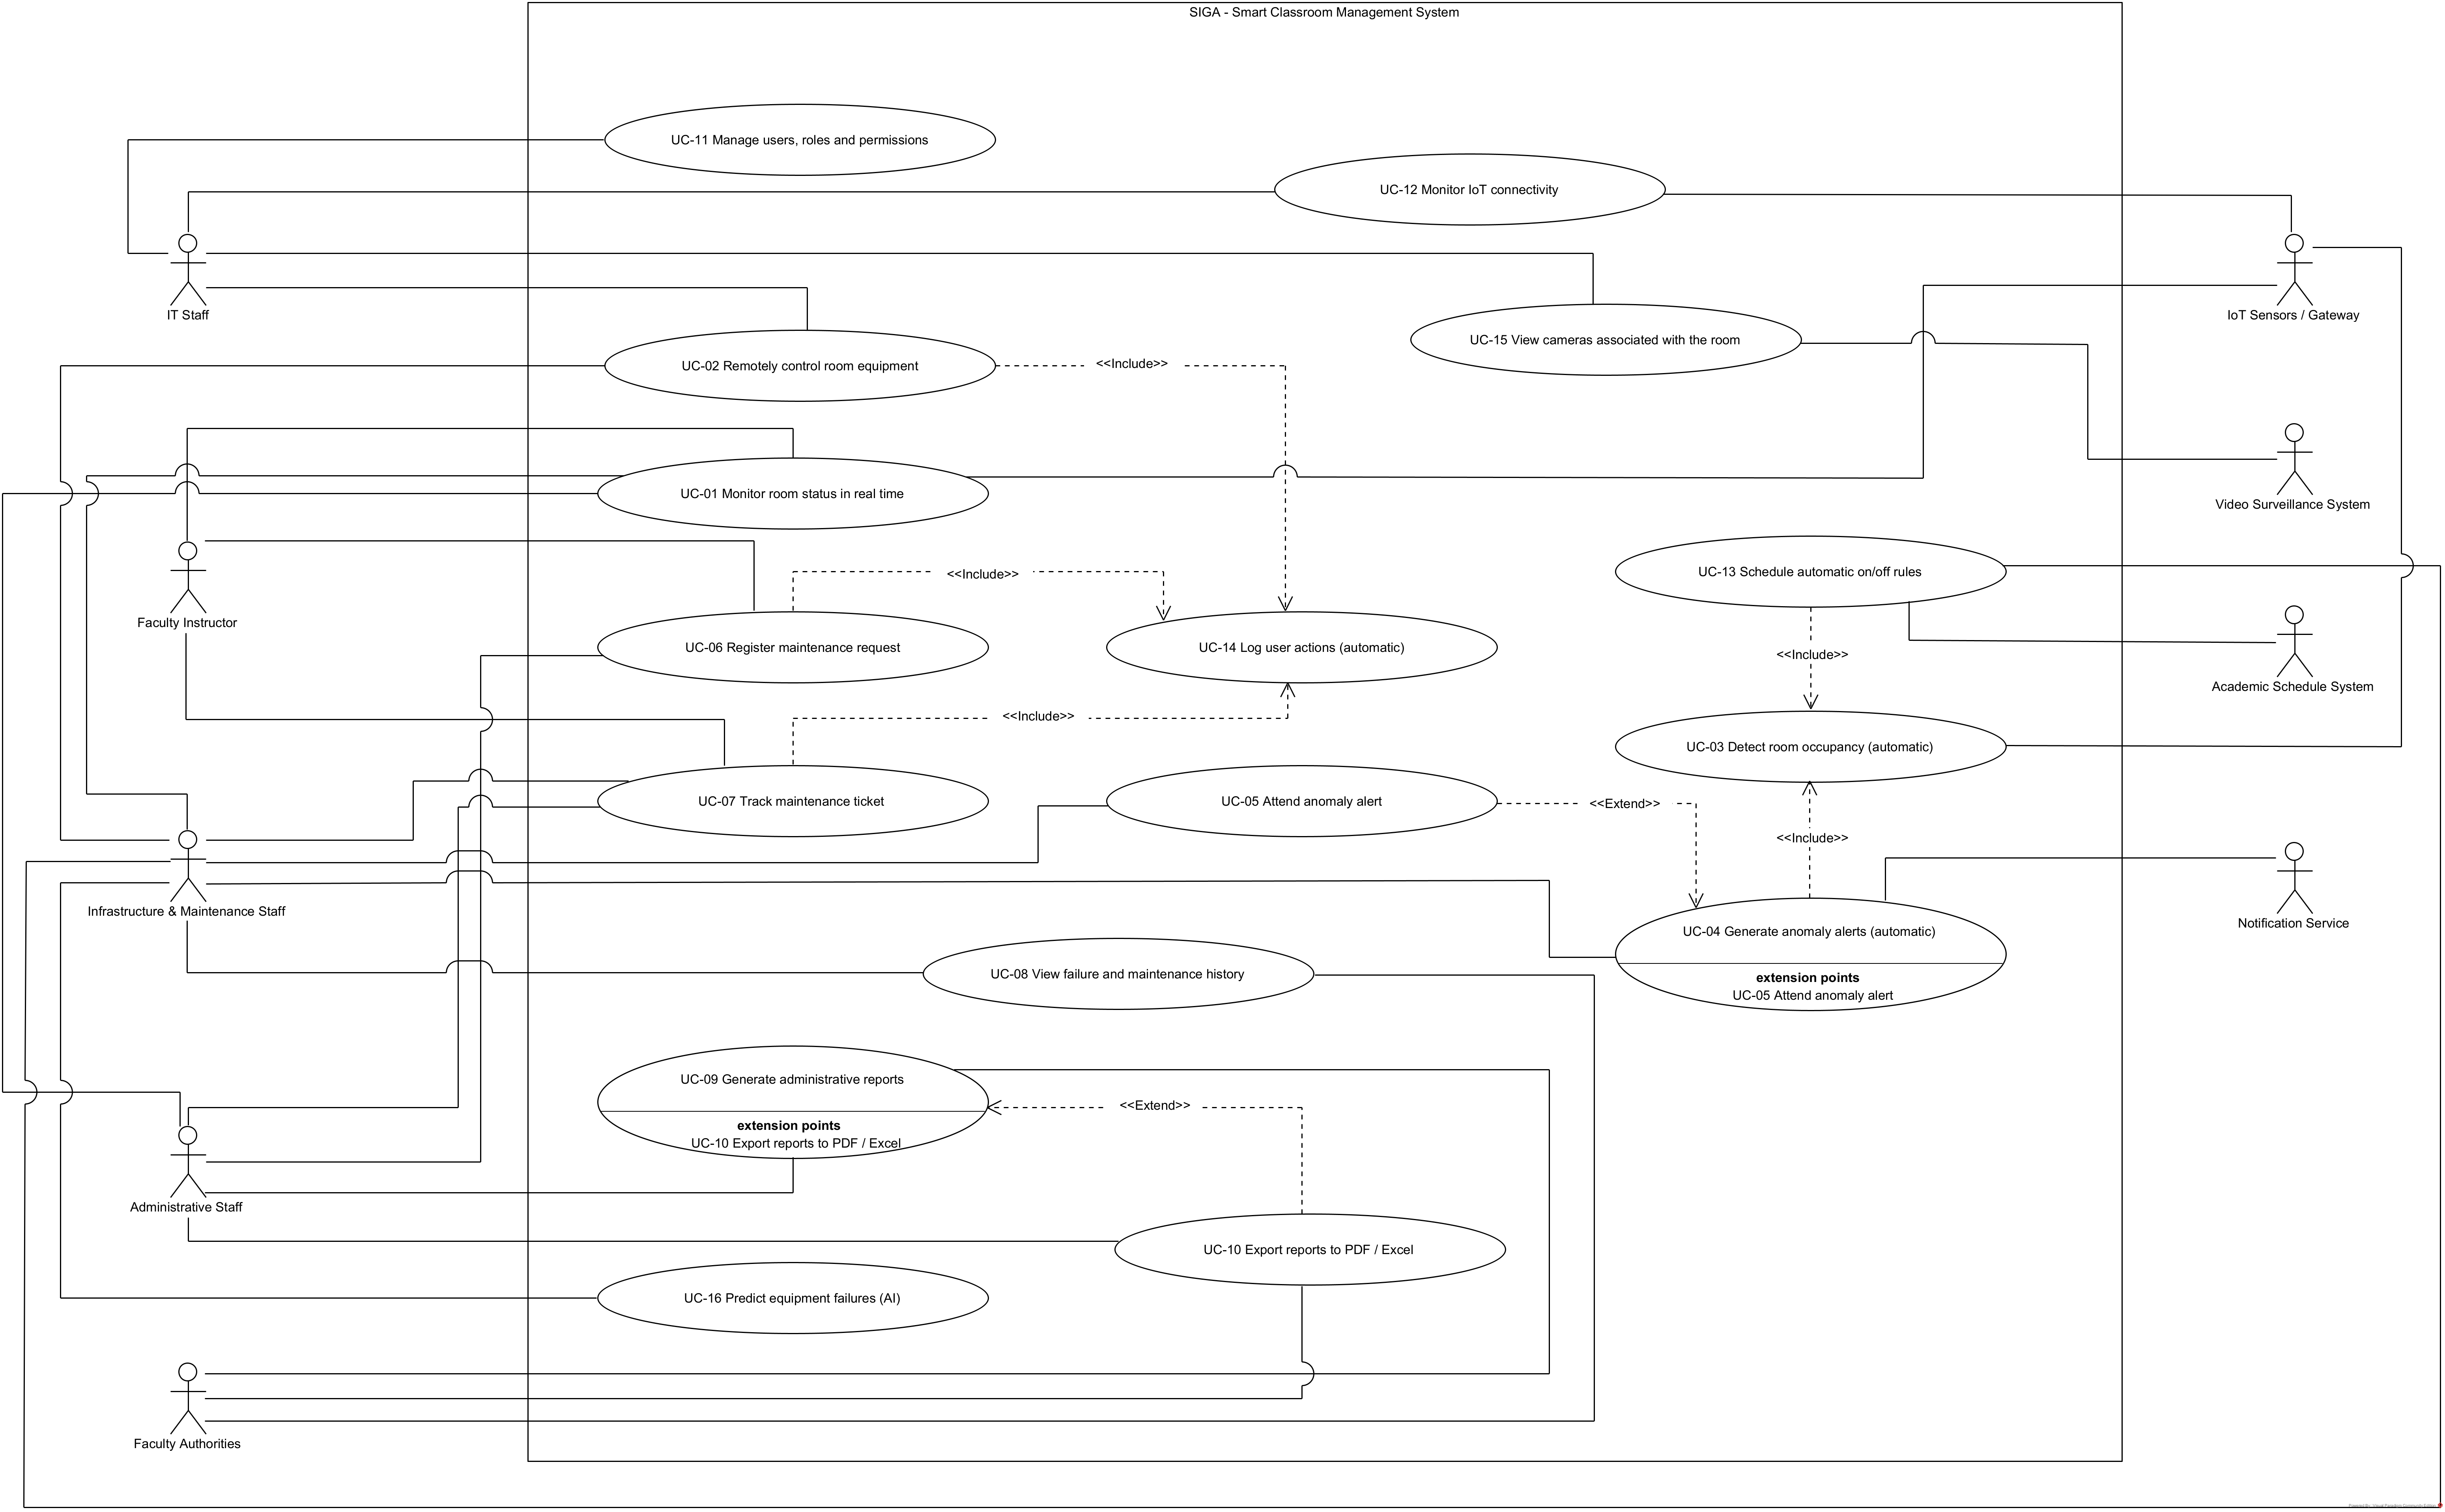
\includegraphics[width=0.85\textwidth,height=0.8\textheight,keepaspectratio]{figuras/usecase_general.png}
\caption{Diagrama de caso de uso general}
\label{fig:img8}
\end{figure}

El diagrama de casos de uso general presenta todos los actores del sistema y el límite del sistema. Los actores humanos (Personal de TI, Docente, Personal de Infraestructura y Mantenimiento, Personal Administrativo, Autoridades de la Facultad) se ubican a la izquierda; los actores de sistema (Sensores/Gateway IoT, Sistema de Videovigilancia, Sistema de Horario Académico, Servicio de Notificaciones) a la derecha. Se identificaron 16 casos de uso cubriendo monitoreo, control, alertas, mantenimiento, reportes y administración.


\subsection*{4.2 Especificación textual de casos de uso detallados}

\addcontentsline{toc}{subsection}{4.2 Especificación textual de casos de uso detallados}

Se presenta la especificación textual completa de los 16 casos de uso identificados en el diagrama general, superando el mínimo de 10 CU detallados exigido por la guía.


\begingroup
\small
\begin{longtable}{|p{7.8cm}|p{7.8cm}|}
\hline
CU-01 | Monitorear estado de aula en tiempo real & CU-01 | Monitorear estado de aula en tiempo real \\ \hline
Actor principal & Personal de Infraestructura y Mantenimiento \\ \hline
Actores secundarios & Docente; Personal Administrativo; Autoridades de la Facultad; Sensores/Gateway IoT \\ \hline
Requisitos relacionados & RF-01, RF-03, RF-04, RF-05, RF-07 \\ \hline
Propósito & Permitir la consulta del estado actualizado de las aulas, incluyendo ocupación, temperatura, humedad, conectividad y estado operativo de equipos. \\ \hline
Precondiciones & El usuario debe estar autenticado en el sistema. / Los sensores y dispositivos IoT deben estar registrados y asociados a un aula. / El aula debe formar parte del conjunto de espacios monitoreados. \\ \hline
Postcondiciones & El sistema muestra el estado actualizado del aula. / Los datos consultados quedan disponibles para alertas, reportes e historial. \\ \hline
Curso normal de eventos & 1. El usuario ingresa al panel de control centralizado. 2. El sistema muestra la lista de aulas monitoreadas. 3. El usuario selecciona un aula o consulta la vista general. 4. El sistema solicita o recibe datos de sensores y dispositivos IoT. 5. El sistema presenta temperatura, humedad, ocupación, estado del proyector, climatización y conectividad. 6. El usuario revisa el estado del aula y determina si existe alguna condición anómala. 7. El sistema mantiene la información actualizada sin requerir recarga manual. \\ \hline
Flujos alternativos / excepciones & A1. Si un sensor no responde, el sistema muestra el estado ``sin conexión'' y puede generar una alerta de conectividad. A2. Si el usuario no tiene permisos, el sistema bloquea el acceso al panel de monitoreo. A3. Si no existen datos recientes, el sistema muestra la última lectura disponible con fecha y hora. \\ \hline
\caption{Especificación textual del caso de uso CU-01: Monitorear estado de aula en tiempo real}
\end{longtable}
\endgroup

\begingroup
\small
\begin{longtable}{|p{7.8cm}|p{7.8cm}|}
\hline
CU-02 | Controlar remotamente equipos de aula & CU-02 | Controlar remotamente equipos de aula \\ \hline
Actor principal & Personal de Infraestructura y Mantenimiento \\ \hline
Actores secundarios & Personal de TI; Sensores/Gateway IoT \\ \hline
Requisitos relacionados & RF-02, RF-04, RF-05, RF-13, RF-16, RF-23 \\ \hline
Propósito & Permitir el encendido, apagado o ajuste remoto de equipos compatibles, como proyectores y climatización. \\ \hline
Precondiciones & El usuario debe estar autenticado con permisos de control remoto. / El equipo debe estar conectado a un controlador compatible. / La red institucional debe permitir la comunicación con el dispositivo. \\ \hline
Postcondiciones & El equipo cambia su estado según el comando enviado. / La acción queda registrada en la bitácora del sistema. \\ \hline
Curso normal de eventos & 1. El usuario ingresa al módulo de control de equipos. 2. El sistema muestra los equipos disponibles por aula. 3. El usuario selecciona el equipo que desea controlar. 4. El usuario envía un comando de encendido, apagado o ajuste. 5. El sistema valida los permisos del usuario. 6. El sistema envía el comando al controlador correspondiente. 7. El controlador ejecuta la acción solicitada. 8. El sistema muestra la confirmación de ejecución. 9. El sistema registra la acción en la bitácora. \\ \hline
Flujos alternativos / excepciones & A1. Si el equipo no está en línea, el sistema informa que no se puede ejecutar el comando. A2. Si el usuario no tiene permisos, el sistema deniega la operación. A3. Si el controlador no confirma la ejecución, el sistema muestra un mensaje de error y registra el intento fallido. \\ \hline
\caption{Especificación textual del caso de uso CU-02: Controlar remotamente equipos de aula}
\end{longtable}
\endgroup

\begingroup
\small
\begin{longtable}{|p{7.8cm}|p{7.8cm}|}
\hline
CU-03 | Detectar ocupación de aula & CU-03 | Detectar ocupación de aula \\ \hline
Actor principal & Sensores/Gateway IoT \\ \hline
Actores secundarios & Sistema de Horario Académico \\ \hline
Requisitos relacionados & RF-03, RF-13, RF-16, RF-20 \\ \hline
Propósito & Determinar si un aula está ocupada o desocupada mediante sensores de presencia u ocupación. \\ \hline
Precondiciones & El sensor de presencia debe estar instalado y configurado. / El sensor debe estar asociado a un aula registrada en el sistema. / La conexión entre sensor, gateway y plataforma debe estar activa. \\ \hline
Postcondiciones & El estado de ocupación del aula queda actualizado. / El evento de ocupación puede utilizarse para alertas, reportes o reglas de apagado automático. \\ \hline
Curso normal de eventos & 1. El sensor detecta presencia, movimiento o ausencia de ocupación. 2. El gateway recibe la señal del sensor. 3. El gateway envía la información a la plataforma SIGA. 4. El sistema interpreta la lectura recibida. 5. El sistema actualiza el estado del aula como ``Ocupada'' o ``Desocupada''. 6. El sistema registra el evento de ocupación con fecha, hora y aula. 7. El estado queda disponible en el panel de control. \\ \hline
Flujos alternativos / excepciones & A1. Si el sensor no responde, el sistema mantiene el último estado conocido y genera una alerta de conectividad. A2. Si la lectura es inconsistente, el sistema marca el evento como pendiente de validación. A3. Si el aula está desocupada fuera de horario, el sistema puede activar reglas de apagado automático. \\ \hline
\caption{Especificación textual del caso de uso CU-03: Detectar ocupación de aula}
\end{longtable}
\endgroup

\begingroup
\small
\begin{longtable}{|p{7.8cm}|p{7.8cm}|}
\hline
CU-04 | Generar alertas por anomalías & CU-04 | Generar alertas por anomalías \\ \hline
Actor principal & Sensores/Gateway IoT \\ \hline
Actores secundarios & Sistema de Horario Académico; Servicio de Notificaciones \\ \hline
Requisitos relacionados & RF-08, RF-11, RF-21, RF-22 \\ \hline
Propósito & Generar alertas automáticas cuando se detecten fallas, condiciones anómalas o equipos encendidos fuera de horario. \\ \hline
Precondiciones & Las reglas de alerta deben estar configuradas. / Los dispositivos deben enviar datos al sistema. / Los responsables de atención deben estar definidos. \\ \hline
Postcondiciones & La alerta queda registrada en el sistema. / El responsable recibe una notificación según la criticidad del evento. \\ \hline
Curso normal de eventos & 1. El sistema recibe una lectura, evento o estado irregular desde un sensor o controlador. 2. El sistema compara el evento con las reglas configuradas. 3. El sistema identifica la anomalía. 4. El sistema clasifica la prioridad de la alerta. 5. El sistema registra la alerta con aula, fecha, hora, tipo de anomalía y responsable sugerido. 6. El sistema envía la notificación al responsable correspondiente. 7. La alerta queda visible en la vista de alertas. \\ \hline
Flujos alternativos / excepciones & A1. Si el evento no supera el umbral definido, el sistema no genera alerta. A2. Si el servicio de notificaciones no está disponible, el sistema registra la alerta como pendiente de envío. A3. Si la alerta ocurre durante una clase activa, el sistema la marca como crítica. \\ \hline
\caption{Especificación textual del caso de uso CU-04: Generar alertas por anomalías}
\end{longtable}
\endgroup

\begingroup
\small
\begin{longtable}{|p{7.8cm}|p{7.8cm}|}
\hline
CU-05 | Atender alerta de anomalía & CU-05 | Atender alerta de anomalía \\ \hline
Actor principal & Personal de Infraestructura y Mantenimiento \\ \hline
Actores secundarios & Personal de TI; Servicio de Notificaciones \\ \hline
Requisitos relacionados & RF-08, RF-10, RF-11, RF-12, RF-23 \\ \hline
Propósito & Permitir que el personal responsable revise, atienda y cierre una alerta generada por el sistema. \\ \hline
Precondiciones & Debe existir una alerta registrada. / El usuario debe estar autenticado con permisos de atención de alertas. \\ \hline
Postcondiciones & La alerta queda actualizada con el estado correspondiente. / La atención queda registrada en el historial y la bitácora. \\ \hline
Curso normal de eventos & 1. El usuario ingresa a la vista de alertas. 2. El sistema muestra las alertas activas y su prioridad. 3. El usuario selecciona una alerta. 4. El sistema muestra el detalle de la anomalía. 5. El usuario revisa el aula, equipo afectado y descripción del evento. 6. El usuario cambia el estado de la alerta a ``En proceso''. 7. El usuario registra la acción realizada o deriva la alerta a un responsable. 8. El sistema actualiza el estado de la alerta. 9. El sistema registra la atención en el historial y la bitácora. \\ \hline
Flujos alternativos / excepciones & A1. Si la alerta requiere mantenimiento, el usuario genera un ticket asociado. A2. Si la alerta corresponde a conectividad, el sistema la deriva al Personal de TI. A3. Si la alerta fue generada por error, el usuario la cierra justificando la causa. \\ \hline
\caption{Especificación textual del caso de uso CU-05: Atender alerta de anomalía}
\end{longtable}
\endgroup

\begingroup
\small
\begin{longtable}{|p{7.8cm}|p{7.8cm}|}
\hline
CU-06 | Registrar solicitud de mantenimiento & CU-06 | Registrar solicitud de mantenimiento \\ \hline
Actor principal & Docente \\ \hline
Actores secundarios & Personal Administrativo; Personal de Infraestructura y Mantenimiento \\ \hline
Requisitos relacionados & RF-12, RF-23 \\ \hline
Propósito & Permitir que un usuario autorizado registre una incidencia relacionada con el aula o sus equipos. \\ \hline
Precondiciones & El usuario debe estar autenticado. / El aula y el equipo afectado deben estar registrados en el sistema. \\ \hline
Postcondiciones & Se genera un ticket de mantenimiento. / La solicitud queda disponible para seguimiento. \\ \hline
Curso normal de eventos & 1. El usuario ingresa al módulo de mantenimiento. 2. El sistema muestra el formulario de solicitud. 3. El usuario selecciona el aula afectada. 4. El usuario selecciona el equipo o componente relacionado. 5. El usuario describe la incidencia. 6. El usuario asigna o confirma la prioridad de la solicitud. 7. El usuario envía la solicitud. 8. El sistema valida los campos requeridos. 9. El sistema genera un ticket con identificador único. 10. El sistema registra la solicitud en la bitácora. \\ \hline
Flujos alternativos / excepciones & A1. Si faltan campos obligatorios, el sistema solicita completar la información. A2. Si el aula no existe, el sistema impide registrar la solicitud. A3. Si la incidencia ya tiene una alerta activa, el sistema permite asociarla al ticket existente. \\ \hline
\caption{Especificación textual del caso de uso CU-06: Registrar solicitud de mantenimiento}
\end{longtable}
\endgroup

\begingroup
\small
\begin{longtable}{|p{7.8cm}|p{7.8cm}|}
\hline
CU-07 | Dar seguimiento a ticket de mantenimiento & CU-07 | Dar seguimiento a ticket de mantenimiento \\ \hline
Actor principal & Personal de Infraestructura y Mantenimiento \\ \hline
Actores secundarios & Docente; Personal Administrativo \\ \hline
Requisitos relacionados & RF-10, RF-12, RF-23 \\ \hline
Propósito & Consultar y actualizar el estado de una solicitud de mantenimiento desde su creación hasta su cierre. \\ \hline
Precondiciones & Debe existir un ticket registrado. / El usuario debe tener permisos para consultar o actualizar el ticket. \\ \hline
Postcondiciones & El ticket queda actualizado. / El cambio de estado queda registrado en el historial. \\ \hline
Curso normal de eventos & 1. El usuario ingresa al módulo de mantenimiento. 2. El sistema muestra la lista de tickets registrados. 3. El usuario selecciona un ticket. 4. El sistema presenta el detalle del ticket y su historial. 5. El usuario actualiza el estado del ticket. 6. El usuario registra una observación o acción realizada. 7. El sistema guarda la actualización. 8. El sistema registra el cambio en la bitácora. 9. El sistema muestra el estado actualizado a los usuarios autorizados. \\ \hline
Flujos alternativos / excepciones & A1. Si el usuario solo tiene permisos de consulta, el sistema bloquea la edición del ticket. A2. Si el ticket ya está cerrado, el sistema solicita justificación para reabrirlo. A3. Si el ticket se deriva a TI, el sistema actualiza el responsable asignado. \\ \hline
\caption{Especificación textual del caso de uso CU-07: Dar seguimiento a ticket de mantenimiento}
\end{longtable}
\endgroup

\begingroup
\small
\begin{longtable}{|p{7.8cm}|p{7.8cm}|}
\hline
CU-08 | Consultar historial de fallas y mantenimientos & CU-08 | Consultar historial de fallas y mantenimientos \\ \hline
Actor principal & Personal de Infraestructura y Mantenimiento \\ \hline
Actores secundarios & Autoridades de la Facultad; Personal Administrativo \\ \hline
Requisitos relacionados & RF-10, RF-17, RF-20 \\ \hline
Propósito & Consultar registros históricos de fallas, mantenimientos e incidencias por aula, equipo o periodo. \\ \hline
Precondiciones & Deben existir registros históricos en el sistema. / El usuario debe estar autenticado y tener permisos de consulta. \\ \hline
Postcondiciones & El sistema presenta el historial filtrado según los criterios ingresados. / La información queda disponible para reportes o análisis administrativo. \\ \hline
Curso normal de eventos & 1. El usuario ingresa al módulo de historial. 2. El sistema muestra los filtros disponibles. 3. El usuario selecciona aula, equipo, tipo de incidencia o rango de fechas. 4. El sistema consulta los registros históricos. 5. El sistema presenta la lista de fallas y mantenimientos encontrados. 6. El usuario revisa el detalle de un registro. 7. El sistema muestra fecha, hora, responsable, acción realizada y estado final. \\ \hline
Flujos alternativos / excepciones & A1. Si no existen registros, el sistema muestra un mensaje informativo. A2. Si el rango de fechas es inválido, el sistema solicita corregirlo. A3. Si el usuario no tiene permisos, el sistema deniega el acceso. \\ \hline
\caption{Especificación textual del caso de uso CU-08: Consultar historial de fallas y mantenimientos}
\end{longtable}
\endgroup

\begingroup
\small
\begin{longtable}{|p{7.8cm}|p{7.8cm}|}
\hline
CU-09 | Generar reportes administrativos & CU-09 | Generar reportes administrativos \\ \hline
Actor principal & Autoridades de la Facultad \\ \hline
Actores secundarios & Personal Administrativo; Personal de Infraestructura y Mantenimiento \\ \hline
Requisitos relacionados & RF-14, RF-17, RF-20 \\ \hline
Propósito & Generar reportes administrativos sobre uso de aulas, ocupación, consumo energético, fallas y estado de equipos. \\ \hline
Precondiciones & Deben existir datos históricos registrados. / El usuario debe tener permisos para generar reportes. \\ \hline
Postcondiciones & El reporte queda generado y disponible para consulta. / Los datos se presentan según los filtros seleccionados. \\ \hline
Curso normal de eventos & 1. El usuario ingresa al módulo de reportes. 2. El sistema muestra los filtros disponibles. 3. El usuario selecciona aula, periodo y tipo de reporte. 4. El sistema valida los criterios ingresados. 5. El sistema recopila los datos históricos correspondientes. 6. El sistema procesa la información. 7. El sistema genera el reporte administrativo. 8. El usuario visualiza indicadores, tablas o resultados consolidados. \\ \hline
Flujos alternativos / excepciones & A1. Si no existen datos para el periodo seleccionado, el sistema muestra un mensaje informativo. A2. Si el usuario no tiene permisos, el sistema impide generar el reporte. A3. Si el reporte requiere exportación, se ejecuta el caso de uso CU-10. \\ \hline
\caption{Especificación textual del caso de uso CU-09: Generar reportes administrativos}
\end{longtable}
\endgroup

\begingroup
\small
\begin{longtable}{|p{7.8cm}|p{7.8cm}|}
\hline
CU-10 | Exportar reportes PDF y Excel & CU-10 | Exportar reportes PDF y Excel \\ \hline
Actor principal & Autoridades de la Facultad \\ \hline
Actores secundarios & Personal Administrativo \\ \hline
Requisitos relacionados & RF-18, RF-23 \\ \hline
Propósito & Exportar reportes administrativos en formatos PDF o Excel para uso institucional. \\ \hline
Precondiciones & Debe existir un reporte generado. / El usuario debe tener permisos de exportación. \\ \hline
Postcondiciones & El archivo queda disponible para descarga. / La exportación queda registrada en la bitácora. \\ \hline
Curso normal de eventos & 1. El usuario visualiza un reporte generado. 2. El usuario selecciona la opción de exportación. 3. El sistema muestra los formatos disponibles. 4. El usuario selecciona PDF o Excel. 5. El sistema genera el archivo en el formato seleccionado. 6. El sistema habilita la descarga del archivo. 7. El sistema registra la acción de exportación. \\ \hline
Flujos alternativos / excepciones & A1. Si el reporte no contiene datos, el sistema impide la exportación. A2. Si ocurre un error al generar el archivo, el sistema muestra un mensaje de error. A3. Si el usuario no tiene permisos, el sistema deniega la acción. \\ \hline
\caption{Especificación textual del caso de uso CU-10: Exportar reportes PDF y Excel}
\end{longtable}
\endgroup

\begingroup
\small
\begin{longtable}{|p{7.8cm}|p{7.8cm}|}
\hline
CU-11 | Gestionar usuarios, roles y permisos & CU-11 | Gestionar usuarios, roles y permisos \\ \hline
Actor principal & Personal de TI \\ \hline
Actores secundarios & Usuarios del sistema \\ \hline
Requisitos relacionados & RF-19, RF-23, NFR-03 \\ \hline
Propósito & Administrar el acceso diferenciado al sistema mediante usuarios, roles y permisos. \\ \hline
Precondiciones & El usuario administrador debe estar autenticado. / Deben existir roles definidos para los perfiles del sistema. \\ \hline
Postcondiciones & El usuario, rol o permiso queda creado, modificado o deshabilitado. / El cambio queda registrado en la bitácora. \\ \hline
Curso normal de eventos & 1. El Personal de TI ingresa al módulo de administración de usuarios. 2. El sistema muestra la lista de usuarios registrados. 3. El usuario selecciona crear, editar o deshabilitar un usuario. 4. El sistema muestra el formulario correspondiente. 5. El usuario asigna rol y permisos. 6. El sistema valida la información ingresada. 7. El sistema guarda los cambios. 8. El sistema registra la acción en la bitácora. \\ \hline
Flujos alternativos / excepciones & A1. Si el usuario ya existe, el sistema informa la duplicidad. A2. Si el rol no tiene permisos definidos, el sistema solicita completarlos. A3. Si se intenta eliminar un usuario con acciones históricas, el sistema permite deshabilitarlo, pero no borrar su trazabilidad. \\ \hline
\caption{Especificación textual del caso de uso CU-11: Gestionar usuarios, roles y permisos}
\end{longtable}
\endgroup

\begingroup
\small
\begin{longtable}{|p{7.8cm}|p{7.8cm}|}
\hline
CU-12 | Monitorear conectividad IoT & CU-12 | Monitorear conectividad IoT \\ \hline
Actor principal & Personal de TI \\ \hline
Actores secundarios & Sensores/Gateway IoT \\ \hline
Requisitos relacionados & RF-22, RF-08 \\ \hline
Propósito & Supervisar la conectividad de sensores, gateways y controladores IoT asociados a las aulas. \\ \hline
Precondiciones & Los dispositivos IoT deben estar registrados en el sistema. / Cada dispositivo debe estar asociado a un aula. \\ \hline
Postcondiciones & El estado de conectividad queda actualizado. / Si existe pérdida de conexión, se genera una alerta. \\ \hline
Curso normal de eventos & 1. El Personal de TI ingresa al módulo de conectividad IoT. 2. El sistema muestra los dispositivos registrados. 3. El sistema consulta el estado de conexión de cada dispositivo. 4. El sistema muestra estado, aula asociada y última comunicación. 5. El usuario revisa los dispositivos con fallas de conexión. 6. El sistema permite filtrar por aula, tipo de dispositivo o estado. \\ \hline
Flujos alternativos / excepciones & A1. Si un dispositivo no responde, el sistema lo marca como ``sin conexión''. A2. Si la pérdida de conexión supera el tiempo configurado, el sistema genera una alerta. A3. Si el dispositivo vuelve a conectarse, el sistema actualiza el estado automáticamente. \\ \hline
\caption{Especificación textual del caso de uso CU-12: Monitorear conectividad IoT}
\end{longtable}
\endgroup

\begingroup
\small
\begin{longtable}{|p{7.8cm}|p{7.8cm}|}
\hline
CU-13 | Programar reglas de encendido y apagado & CU-13 | Programar reglas de encendido y apagado \\ \hline
Actor principal & Personal de Infraestructura y Mantenimiento \\ \hline
Actores secundarios & Sistema de Horario Académico; Sensores/Gateway IoT \\ \hline
Requisitos relacionados & RF-13, RF-15, RF-16, RF-21 \\ \hline
Propósito & Configurar reglas automáticas para encendido y apagado de equipos según horario académico, ocupación o estado del aula. \\ \hline
Precondiciones & El usuario debe tener permisos de configuración. / El horario académico debe estar disponible en formato digital o estructurado. / Los equipos deben ser compatibles con control remoto. \\ \hline
Postcondiciones & La regla queda registrada y activa. / Los equipos se controlan automáticamente según las condiciones definidas. \\ \hline
Curso normal de eventos & 1. El usuario ingresa al módulo de programación de reglas. 2. El sistema muestra las aulas y equipos disponibles. 3. El usuario selecciona el aula y equipo. 4. El usuario define condición de horario, ocupación o estado del equipo. 5. El usuario configura la acción automática. 6. El sistema valida la regla. 7. El sistema guarda la programación. 8. El sistema ejecuta la regla cuando se cumplen las condiciones. \\ \hline
Flujos alternativos / excepciones & A1. Si el horario académico no está disponible, el sistema impide programar reglas dependientes del horario. A2. Si el equipo no es compatible, el sistema informa que no puede ser automatizado. A3. Si existen reglas contradictorias, el sistema solicita ajustar la configuración. \\ \hline
\caption{Especificación textual del caso de uso CU-13: Programar reglas de encendido y apagado}
\end{longtable}
\endgroup

\begingroup
\small
\begin{longtable}{|p{7.8cm}|p{7.8cm}|}
\hline
CU-14 | Registrar bitácora de acciones & CU-14 | Registrar bitácora de acciones \\ \hline
Actor principal & Sistema SIGA \\ \hline
Actores secundarios & Usuarios autenticados \\ \hline
Requisitos relacionados & RF-23 \\ \hline
Propósito & Registrar automáticamente las acciones relevantes realizadas por los usuarios dentro de la plataforma. \\ \hline
Precondiciones & El usuario debe estar autenticado. / Debe ejecutarse una acción relevante dentro del sistema. \\ \hline
Postcondiciones & La acción queda registrada con usuario, fecha, hora, módulo, acción y resultado. / La bitácora queda disponible para consulta autorizada. \\ \hline
Curso normal de eventos & 1. Un usuario ejecuta una acción en la plataforma. 2. El sistema identifica el usuario, rol y módulo afectado. 3. El sistema registra la fecha y hora de la acción. 4. El sistema registra el resultado de la operación. 5. El sistema guarda el evento en la bitácora. 6. La bitácora queda disponible para auditoría. \\ \hline
Flujos alternativos / excepciones & A1. Si la acción falla, el sistema registra el intento y el error generado. A2. Si la sesión expira, el sistema registra el cierre o bloqueo de sesión. A3. Si el evento no es crítico, el sistema puede registrarlo con prioridad informativa. \\ \hline
\caption{Especificación textual del caso de uso CU-14: Registrar bitácora de acciones}
\end{longtable}
\endgroup

\begingroup
\small
\begin{longtable}{|p{7.8cm}|p{7.8cm}|}
\hline
CU-15 | Consultar cámaras asociadas al aula & CU-15 | Consultar cámaras asociadas al aula \\ \hline
Actor principal & Personal de TI \\ \hline
Actores secundarios & Sistema de Videovigilancia; Personal de Infraestructura y Mantenimiento \\ \hline
Requisitos relacionados & RF-06, NFR-03 \\ \hline
Propósito & Consultar una vista complementaria de cámaras asociadas a un aula, siempre que exista autorización técnica e institucional. \\ \hline
Precondiciones & La cámara debe estar operativa. / El sistema de videovigilancia debe permitir acceso autorizado. / El usuario debe contar con permisos para consultar la vista de cámaras. \\ \hline
Postcondiciones & El sistema muestra la vista complementaria o enlace de cámara. / El acceso queda registrado según políticas de seguridad. \\ \hline
Curso normal de eventos & 1. El usuario ingresa al detalle de un aula. 2. El sistema muestra si existe cámara asociada. 3. El usuario selecciona la opción de consultar cámara. 4. El sistema solicita el enlace o flujo autorizado al sistema de videovigilancia. 5. El sistema muestra la vista complementaria dentro del panel o mediante enlace autorizado. 6. El sistema registra el acceso en la bitácora. \\ \hline
Flujos alternativos / excepciones & A1. Si la cámara no está disponible, el sistema muestra un mensaje de indisponibilidad. A2. Si el usuario no tiene permisos, el sistema bloquea el acceso. A3. Si el flujo de video presenta latencia o error, el sistema informa la falla técnica. \\ \hline
\caption{Especificación textual del caso de uso CU-15: Consultar cámaras asociadas al aula}
\end{longtable}
\endgroup

\begingroup
\small
\begin{longtable}{|p{7.8cm}|p{7.8cm}|}
\hline
CU-16 | Predecir fallas de equipos & CU-16 | Predecir fallas de equipos \\ \hline
Actor principal & Personal de Infraestructura y Mantenimiento \\ \hline
Actores secundarios & Autoridades de la Facultad; Sensores/Gateway IoT \\ \hline
Requisitos relacionados & RF-09, RF-10, RF-14, RF-17 \\ \hline
Propósito & Analizar datos históricos de uso, fallas y mantenimiento para estimar posibles fallas futuras en equipos de aula. \\ \hline
Precondiciones & El sistema debe contar con datos históricos suficientes. / Los equipos deben tener registros de uso, fallas o mantenimiento. / El usuario debe tener permisos para consultar análisis predictivo. \\ \hline
Postcondiciones & El sistema muestra un indicador de riesgo por equipo o aula. / La información puede utilizarse para planificación de mantenimiento preventivo. \\ \hline
Curso normal de eventos & 1. El usuario ingresa al módulo de análisis predictivo. 2. El sistema muestra las aulas y equipos disponibles para análisis. 3. El usuario selecciona aula, equipo o periodo de análisis. 4. El sistema consulta datos históricos de fallas, uso, consumo y mantenimiento. 5. El sistema procesa los datos mediante el módulo de análisis. 6. El sistema genera un indicador de riesgo bajo, medio o alto. 7. El sistema muestra la recomendación de mantenimiento preventivo. 8. El usuario revisa el resultado y decide si genera una acción de mantenimiento. \\ \hline
Flujos alternativos / excepciones & A1. Si no existen datos históricos suficientes, el sistema informa que no puede generar predicción confiable. A2. Si el equipo no tiene historial, el sistema lo excluye del análisis predictivo. A3. Si el riesgo es alto, el sistema permite generar una alerta o ticket preventivo. \\ \hline
\caption{Especificación textual del caso de uso CU-16: Predecir fallas de equipos}
\end{longtable}
\endgroup

\subsection*{4.3 Diagrama de clases refinado}

\addcontentsline{toc}{subsection}{4.3 Diagrama de clases refinado}

El diagrama de clases parte del modelo conceptual de la Entrega 1B (16 clases: Aula, SensorIoT, LecturaSensor, Equipo, Proyector, Climatizador, GatewayIoT, Alerta, SolicitudMantenimiento, Usuario, Rol, HorarioAcademico, ConsumoEnergetico, ReporteAdministrativo, BitacoraAccion, CamaraVigilancia) y se refina agregando atributos tipados y operaciones a cada clase.


\begin{figure}[H]
\centering
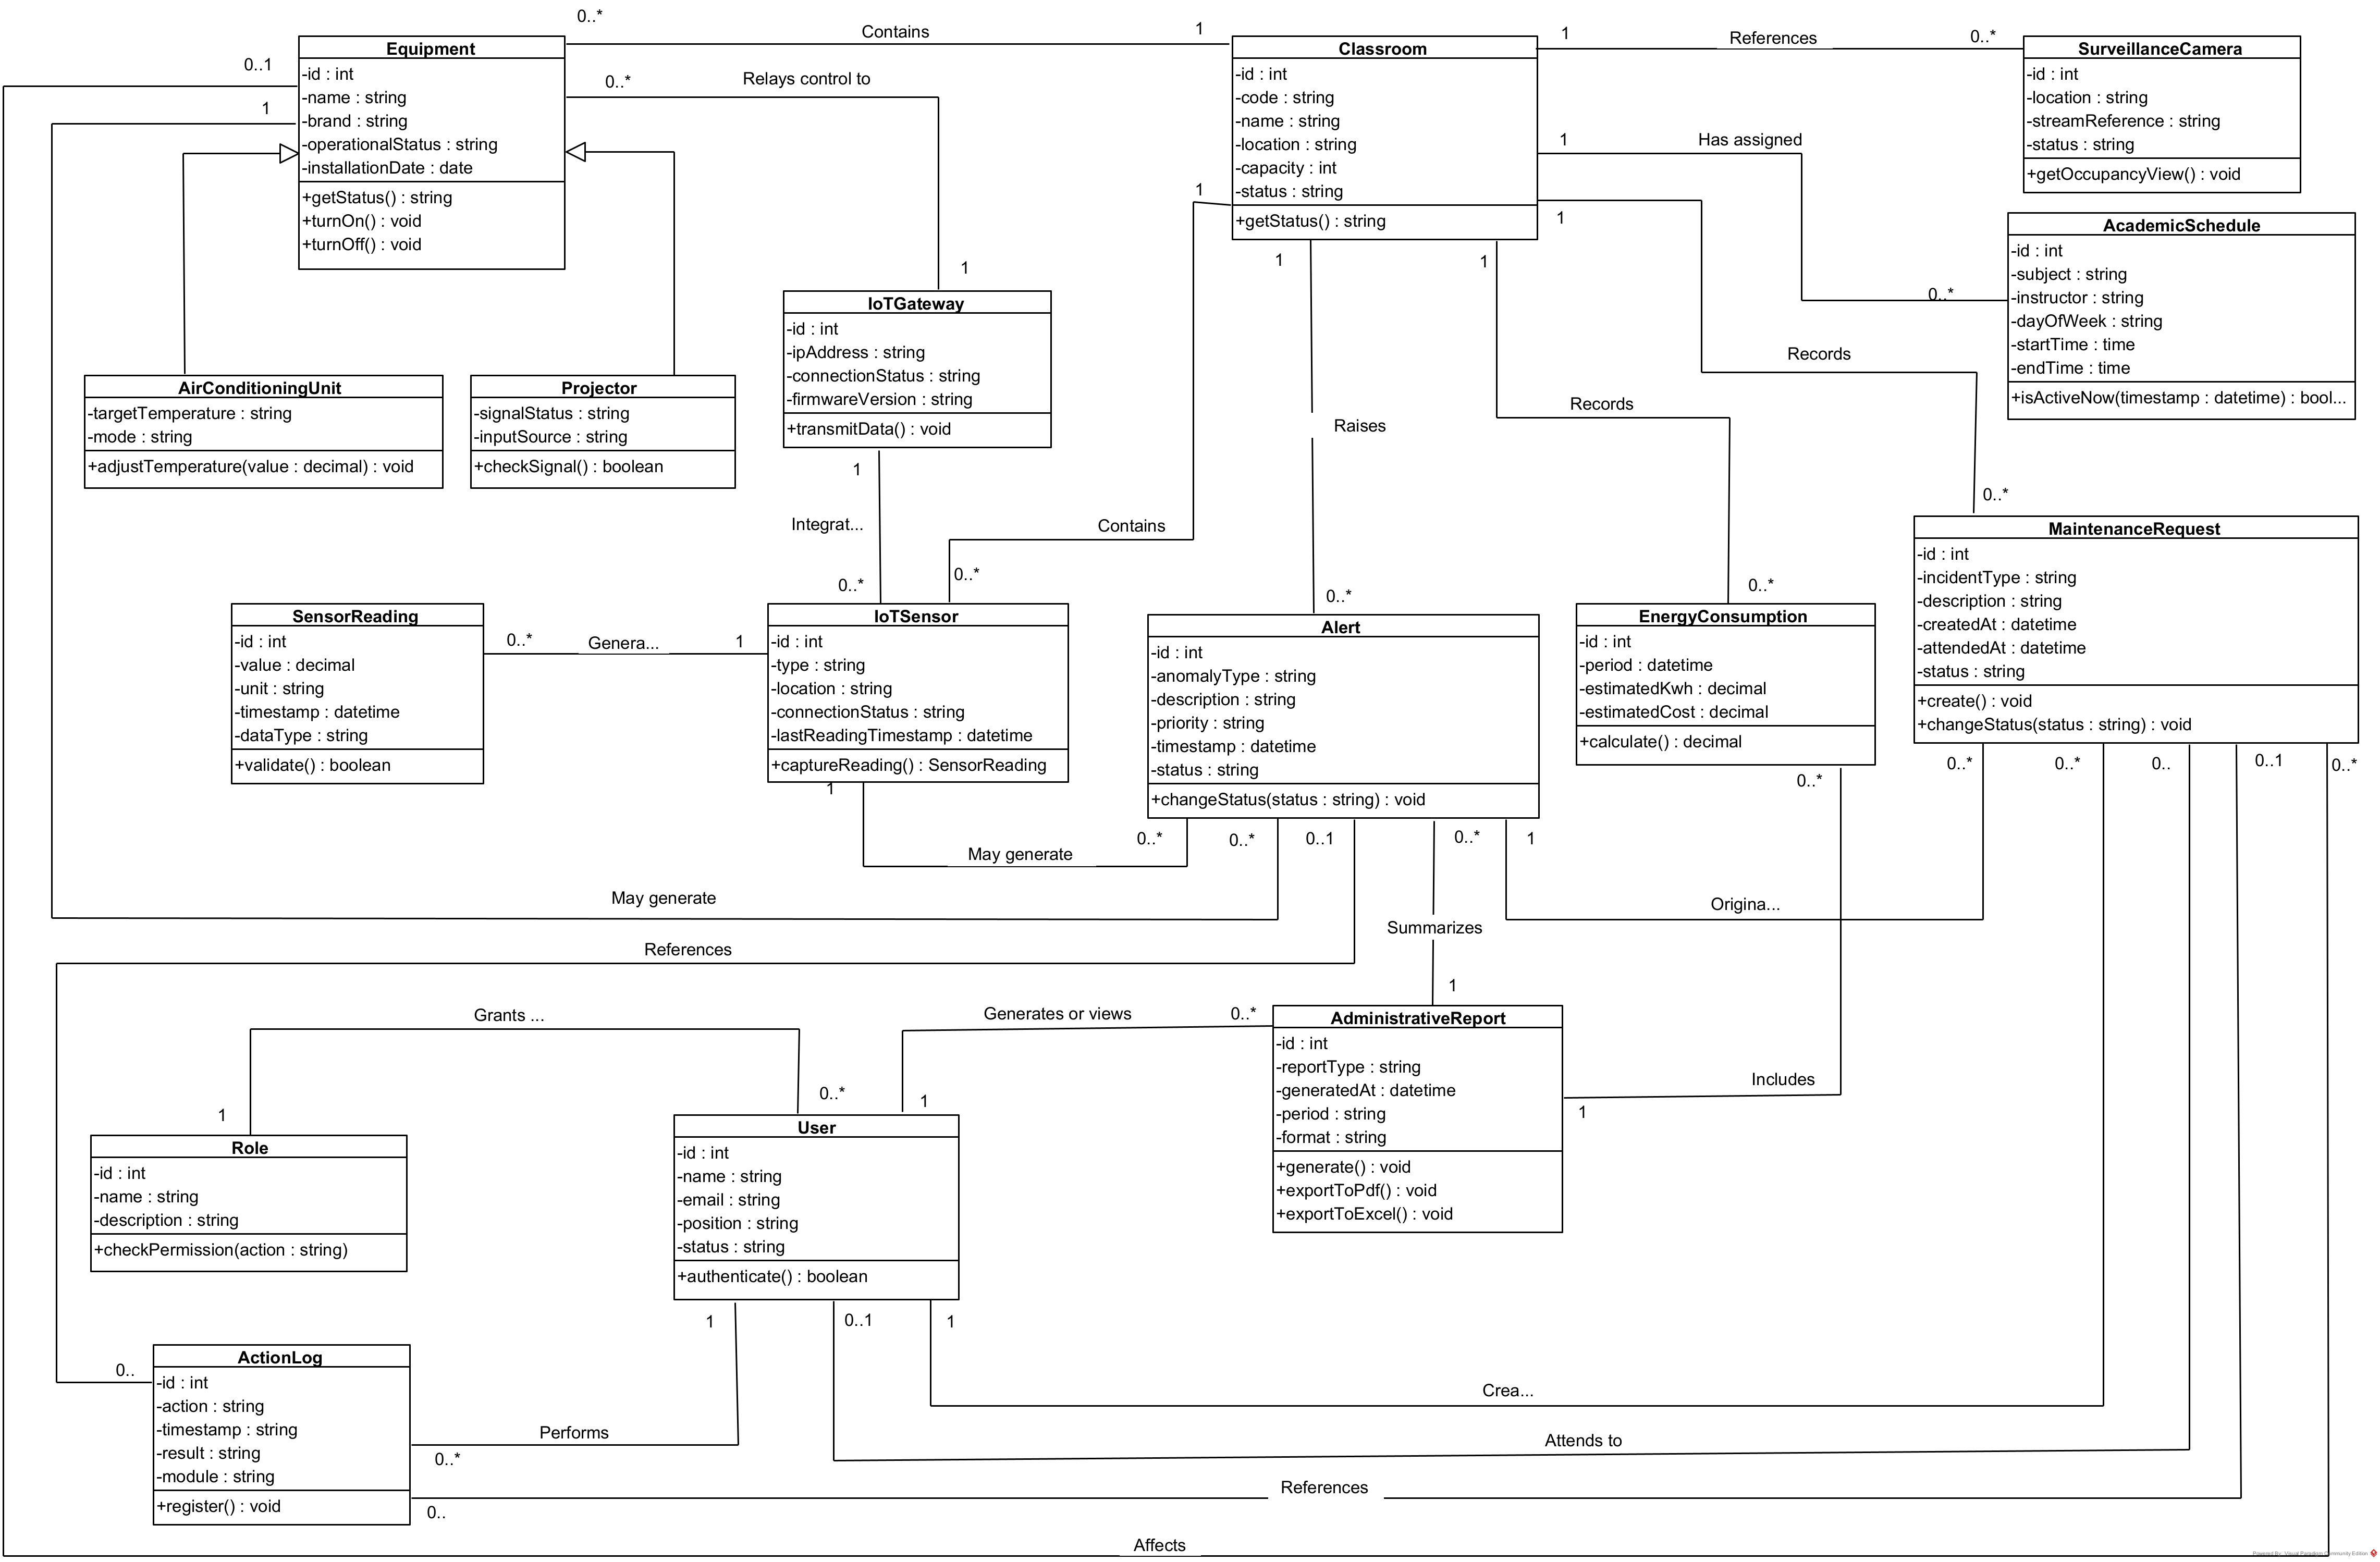
\includegraphics[width=0.85\textwidth,height=0.8\textheight,keepaspectratio]{figuras/class_diagram_refined.png}
\caption{Diagrama de clases refinado}
\label{fig:img9}
\end{figure}

Especificación de refinamiento sugerida: Aula(id: int, nombre: string, capacidad: int, ubicacion: string) + metodos consultarEstado(), registrarOcupacion(). SensorIoT(id: int, tipo: string, aula\_id: int, estado: string) + metodos enviarLectura(), verificarConexion(). Equipo(id: int, tipo: string, estado: string) como clase base de Proyector(resolucion: string, entrada: string) y Climatizador(temperaturaObjetivo: float) mediante herencia. Alerta(id: int, tipo: string, prioridad: string, fecha: datetime, estado: string) + metodos generar(), cerrar(). SolicitudMantenimiento(id: int, descripcion: string, prioridad: string, estado: string) + metodos crear(), actualizarEstado(). Usuario(id: int, nombre: string, correo: string, rol\_id: int) + metodos autenticar(), exportarDatos(), rectificarDatos() --- estas dos últimas operaciones soportan RF-24 y RF-25.


\subsection*{4.4 Diagramas de secuencia}

\addcontentsline{toc}{subsection}{4.4 Diagramas de secuencia}

Nuevo en esta entrega. Se especifican para los casos de uso críticos:


\textit{Secuencia CU-04 (Generar alertas): }\textit{SensorIoT}\textit{ $\rightarrow$ }\textit{GatewayIoT}\textit{ $\rightarrow$ }\textit{SIGA.evaluarRegla}\textit{() $\rightarrow$ }\textit{SIGA.crearAlerta}\textit{() $\rightarrow$ }\textit{ServicioNotificaciones.enviar}\textit{() $\rightarrow$ }\textit{PersonalInfraestructura.recibirAlerta}\textit{().}


\textit{Secuencia CU-06 (Registrar solicitud de mantenimiento): Docente $\rightarrow$ }\textit{SIGA.mostrarFormulario}\textit{() $\rightarrow$ }\textit{Docente.enviarSolicitud}\textit{() $\rightarrow$ }\textit{SIGA.validarCampos}\textit{() $\rightarrow$ }\textit{SIGA.generarTicket}\textit{() $\rightarrow$ }\textit{BitacoraAccion.registrar}\textit{().}


\textit{Secuencia CU-16 (Predecir fallas, RF-09): }\textit{PersonalInfraestructura}\textit{ $\rightarrow$ }\textit{SIGA.solicitarAnalisis}\textit{() $\rightarrow$ }\textit{SIGA.consultarHistorico}\textit{() $\rightarrow$ }\textit{ModuloIA.procesarDatos}\textit{() $\rightarrow$ }\textit{ModuloIA.generarIndicadorRiesgo}\textit{() $\rightarrow$ }\textit{ModuloIA.generarExplicacion}\textit{() [RNF-10] $\rightarrow$ }\textit{SIGA.mostrarResultado}\textit{().}


\begin{figure}[H]
\centering
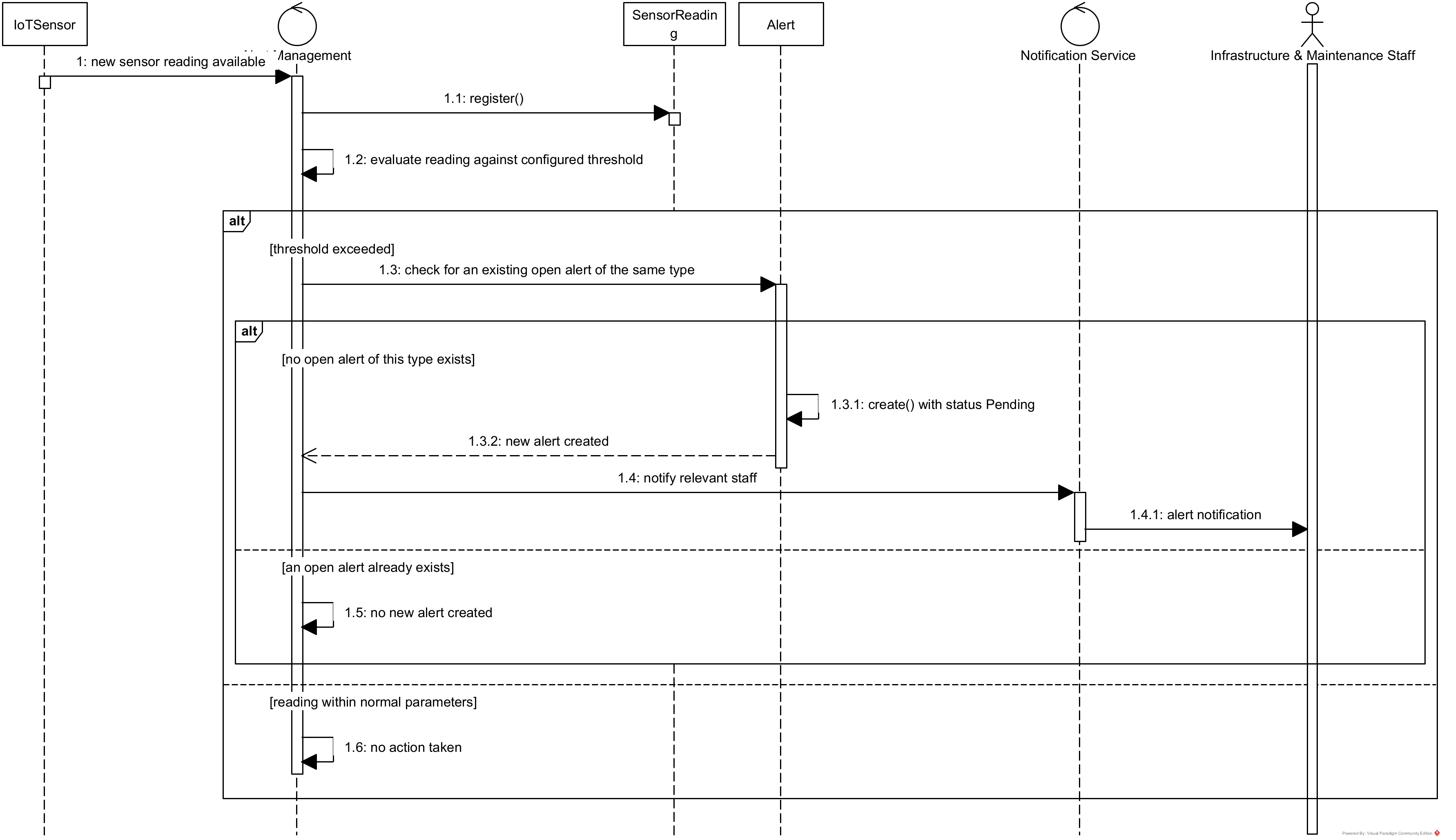
\includegraphics[width=0.85\textwidth,height=0.8\textheight,keepaspectratio]{figuras/seq_UC04_generate_anomaly_alerts.png}
\caption{Diagrama de secuencia --- CU-04 Generar alertas por anomalías}
\label{fig:img10}
\end{figure}

\begin{figure}[H]
\centering
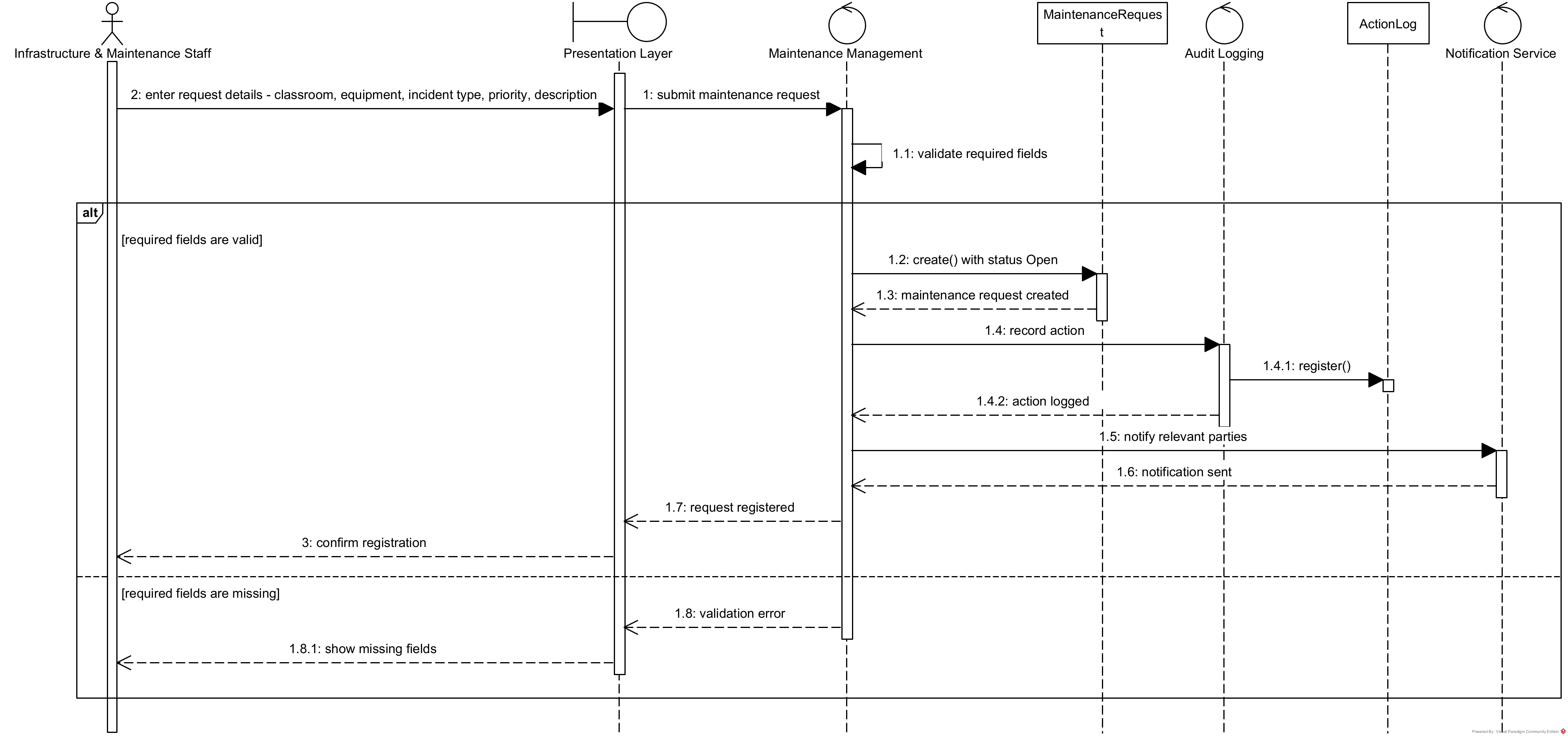
\includegraphics[width=0.85\textwidth,height=0.8\textheight,keepaspectratio]{figuras/seq_UC06_register_maintenance_request.png}
\caption{Diagrama de secuencia --- CU-06 Registrar solicitud de mantenimiento}
\label{fig:img11}
\end{figure}

\begin{figure}[H]
\centering
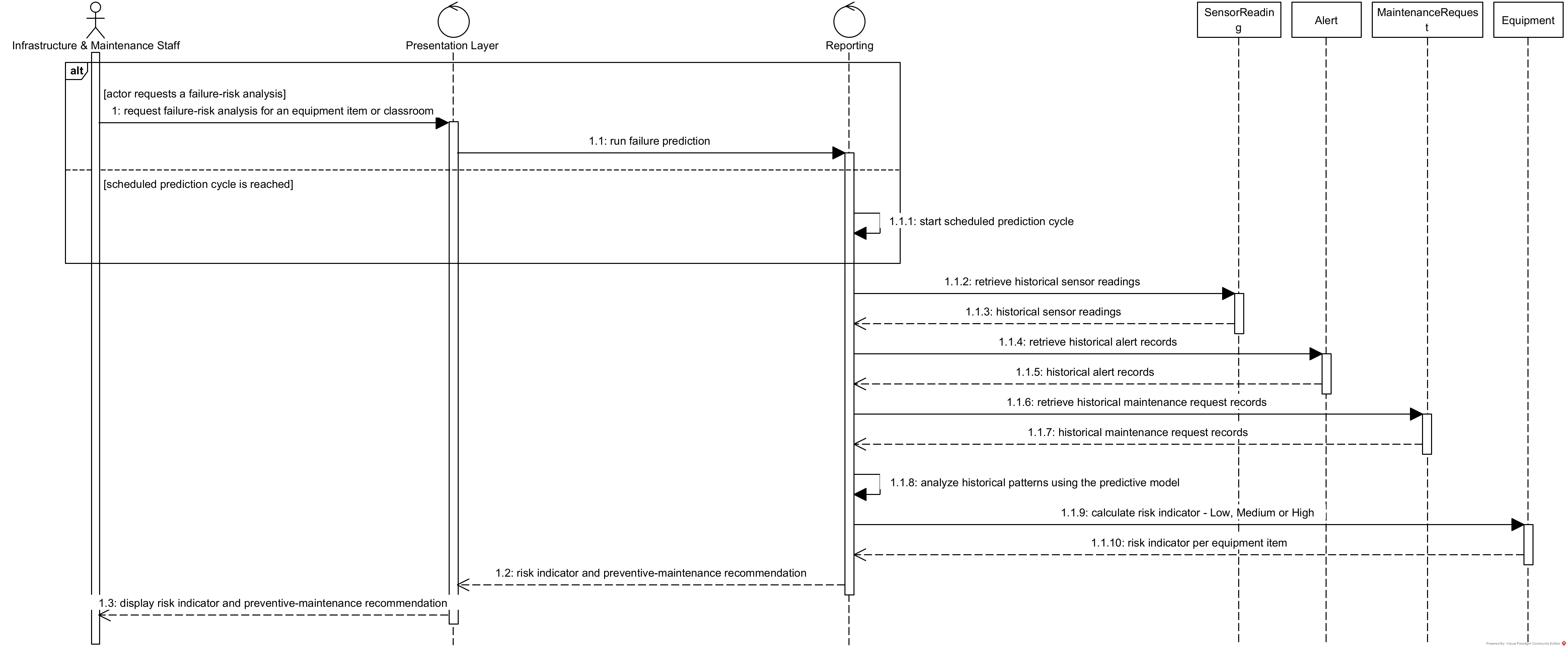
\includegraphics[width=0.85\textwidth,height=0.8\textheight,keepaspectratio]{figuras/seq_UC16_predict_equipment_failures.png}
\caption{Diagrama de secuencia --- CU-16 Predecir fallas de equipos (RF-09, explicabilidad RNF-10)}
\label{fig:img12}
\end{figure}

\subsection*{4.5 Diagramas de actividad}

\addcontentsline{toc}{subsection}{4.5 Diagramas de actividad}

\textit{Flujo de atención de alerta (CU-04 $\rightarrow$ CU-05): Inicio $\rightarrow$ Sensor detecta anomalía $\rightarrow$ Sistema evalúa regla $\rightarrow$ [¿Supera umbral?] $\rightarrow$ Sí: genera alerta y notifica $\rightarrow$ }\textit{Responsable}\textit{ atiende $\rightarrow$ [¿Requiere mantenimiento?] $\rightarrow$ Sí: genera }\textit{ticket}\textit{ (CU-06) / No: cierra alerta $\rightarrow$ Fin.}


\textit{Flujo de }\textit{ticket}\textit{ de mantenimiento (CU-06 $\rightarrow$ CU-07): Inicio $\rightarrow$ Usuario registra solicitud $\rightarrow$ Sistema valida campos $\rightarrow$ Sistema genera }\textit{ticket}\textit{ $\rightarrow$ Personal de Infraestructura revisa $\rightarrow$ Actualiza estado $\rightarrow$ [¿Resuelto?] $\rightarrow$ Sí: cierra }\textit{ticket}\textit{ / No: continúa seguimiento $\rightarrow$ Fin.}


\begin{figure}[H]
\centering
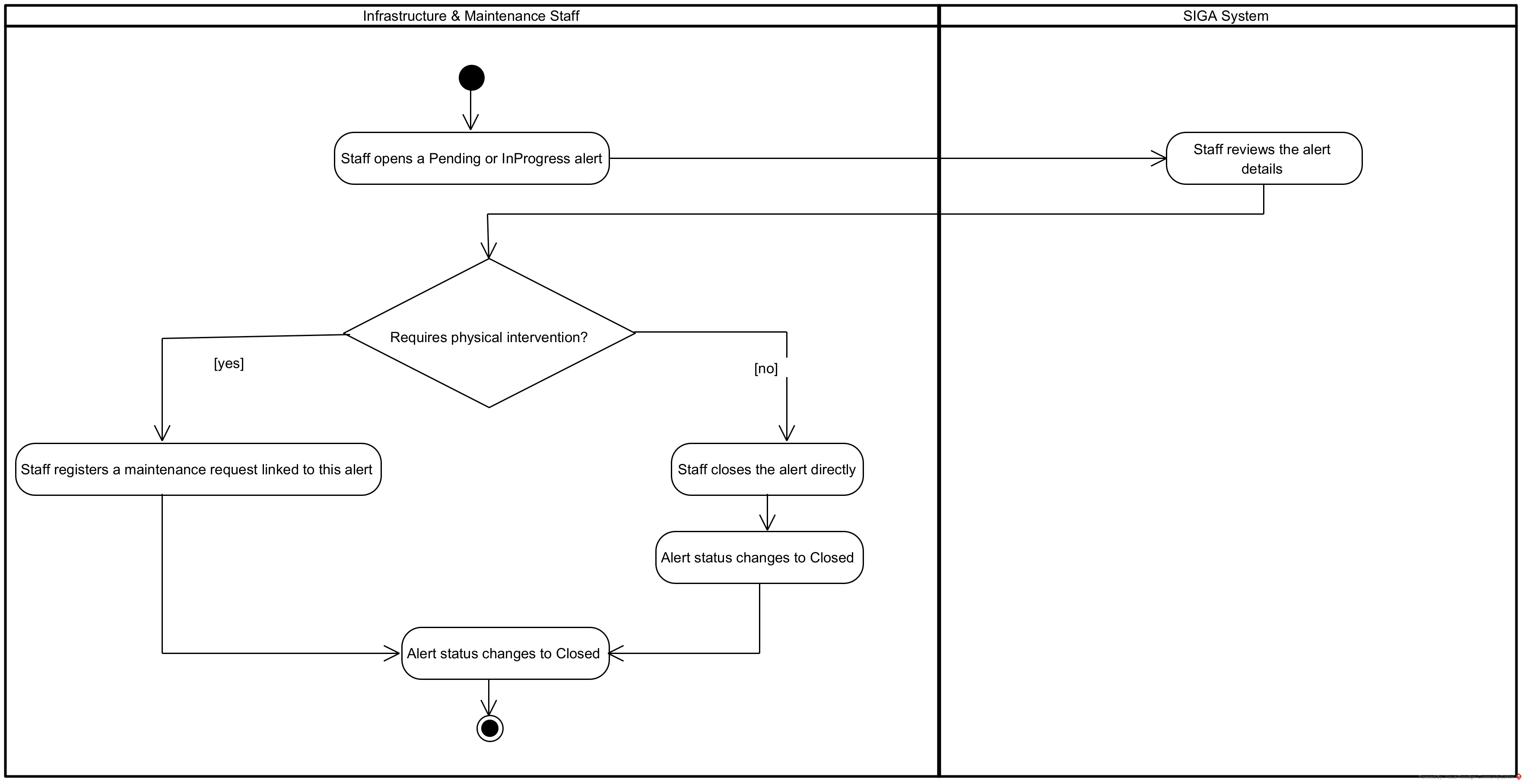
\includegraphics[width=0.85\textwidth,height=0.8\textheight,keepaspectratio]{figuras/act_UC05_attend_anomaly_alert.png}
\caption{Diagrama de actividad --- Atención de alerta (CU-04 $\rightarrow$ CU-05)}
\label{fig:img13}
\end{figure}

\begin{figure}[H]
\centering
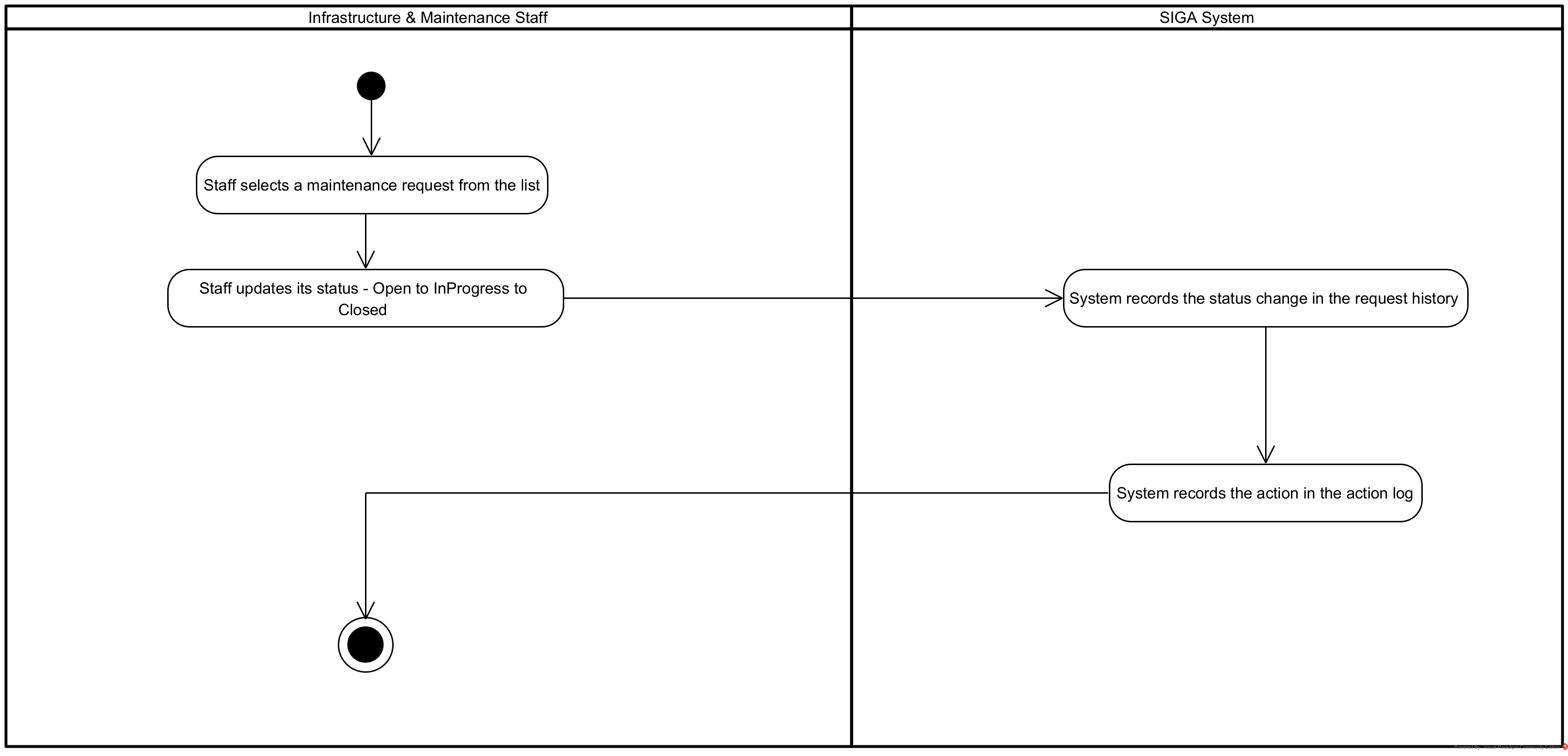
\includegraphics[width=0.85\textwidth,height=0.8\textheight,keepaspectratio]{figuras/act_UC07_track_maintenance_ticket.png}
\caption{Diagrama de actividad --- Ticket de mantenimiento (CU-06 $\rightarrow$ CU-07)}
\label{fig:img14}
\end{figure}

\subsection*{4.6 Diagrama de estados}

\addcontentsline{toc}{subsection}{4.6 Diagrama de estados}

\textit{Entidad seleccionada: }\textit{SolicitudMantenimiento}\textit{, por ser la entidad con ciclo de vida no trivial más representativo del dominio. Estados: Registrada $\rightarrow$ En proceso $\rightarrow$ \{Resuelta | Cancelada\}. Transiciones: Registrada $\rightarrow$ En proceso (asignación de responsable); En proceso $\rightarrow$ Resuelta (cierre con acción registrada); En proceso $\rightarrow$ Cancelada (justificación registrada); Resuelta $\rightarrow$ En proceso (reapertura justificada, ver CU-07 flujo alternativo A2).}


\begin{figure}[H]
\centering
\includegraphics[width=0.85\textwidth,height=0.8\textheight,keepaspectratio]{figuras/state_maintenance_request.png}
\caption{Diagrama de estados --- SolicitudMantenimiento}
\label{fig:img15}
\end{figure}

\subsection*{4.7 Diagrama de componentes}

\addcontentsline{toc}{subsection}{4.7 Diagrama de componentes}

\textit{Componentes propuestos: }\textit{Frontend}\textit{ Web (panel de control, alertas, mantenimiento, reportes), API REST (orquesta la comunicación entre }\textit{frontend}\textit{, base de datos y servicios), Servicio de Análisis IA (RF-09, RF-14, RNF-10), Gateway }\textit{IoT}\textit{ (concentra sensores y controladores), Base de Datos, Servicio de Notificaciones. Las dependencias principales: }\textit{Frontend}\textit{ $\rightarrow$ API REST $\rightarrow$ \{Base de Datos, Servicio de Análisis IA, Servicio de Notificaciones\}; Gateway }\textit{IoT}\textit{ $\rightarrow$ API REST.}


\begin{figure}[H]
\centering

\includegraphics[width=0.85\textwidth,height=0.8\textheight,keepaspectratio]{figuras/component_diagram.png}
\caption{Diagrama de componentes --- SIGA}
\label{fig:img16}
\end{figure}

\subsection*{4.8 Diagrama de despliegue}

\addcontentsline{toc}{subsection}{4.8 Diagrama de despliegue}

\textit{Nodos físicos propuestos: Servidor institucional o }\textit{cloud}\textit{ (aloja API REST, base de datos, servicio de análisis IA); Gateway }\textit{IoT}\textit{ por aula piloto (conecta sensores y controladores vía MQTT); Dispositivos cliente (navegador web, protocolo HTTPS). Protocolos entre nodos: MQTT (sensores $\rightarrow$ }\textit{gateway}\textit{), API REST/HTTPS (}\textit{gateway}\textit{ $\rightarrow$ servidor, cliente $\rightarrow$ servidor).}


\begin{figure}[H]
\centering
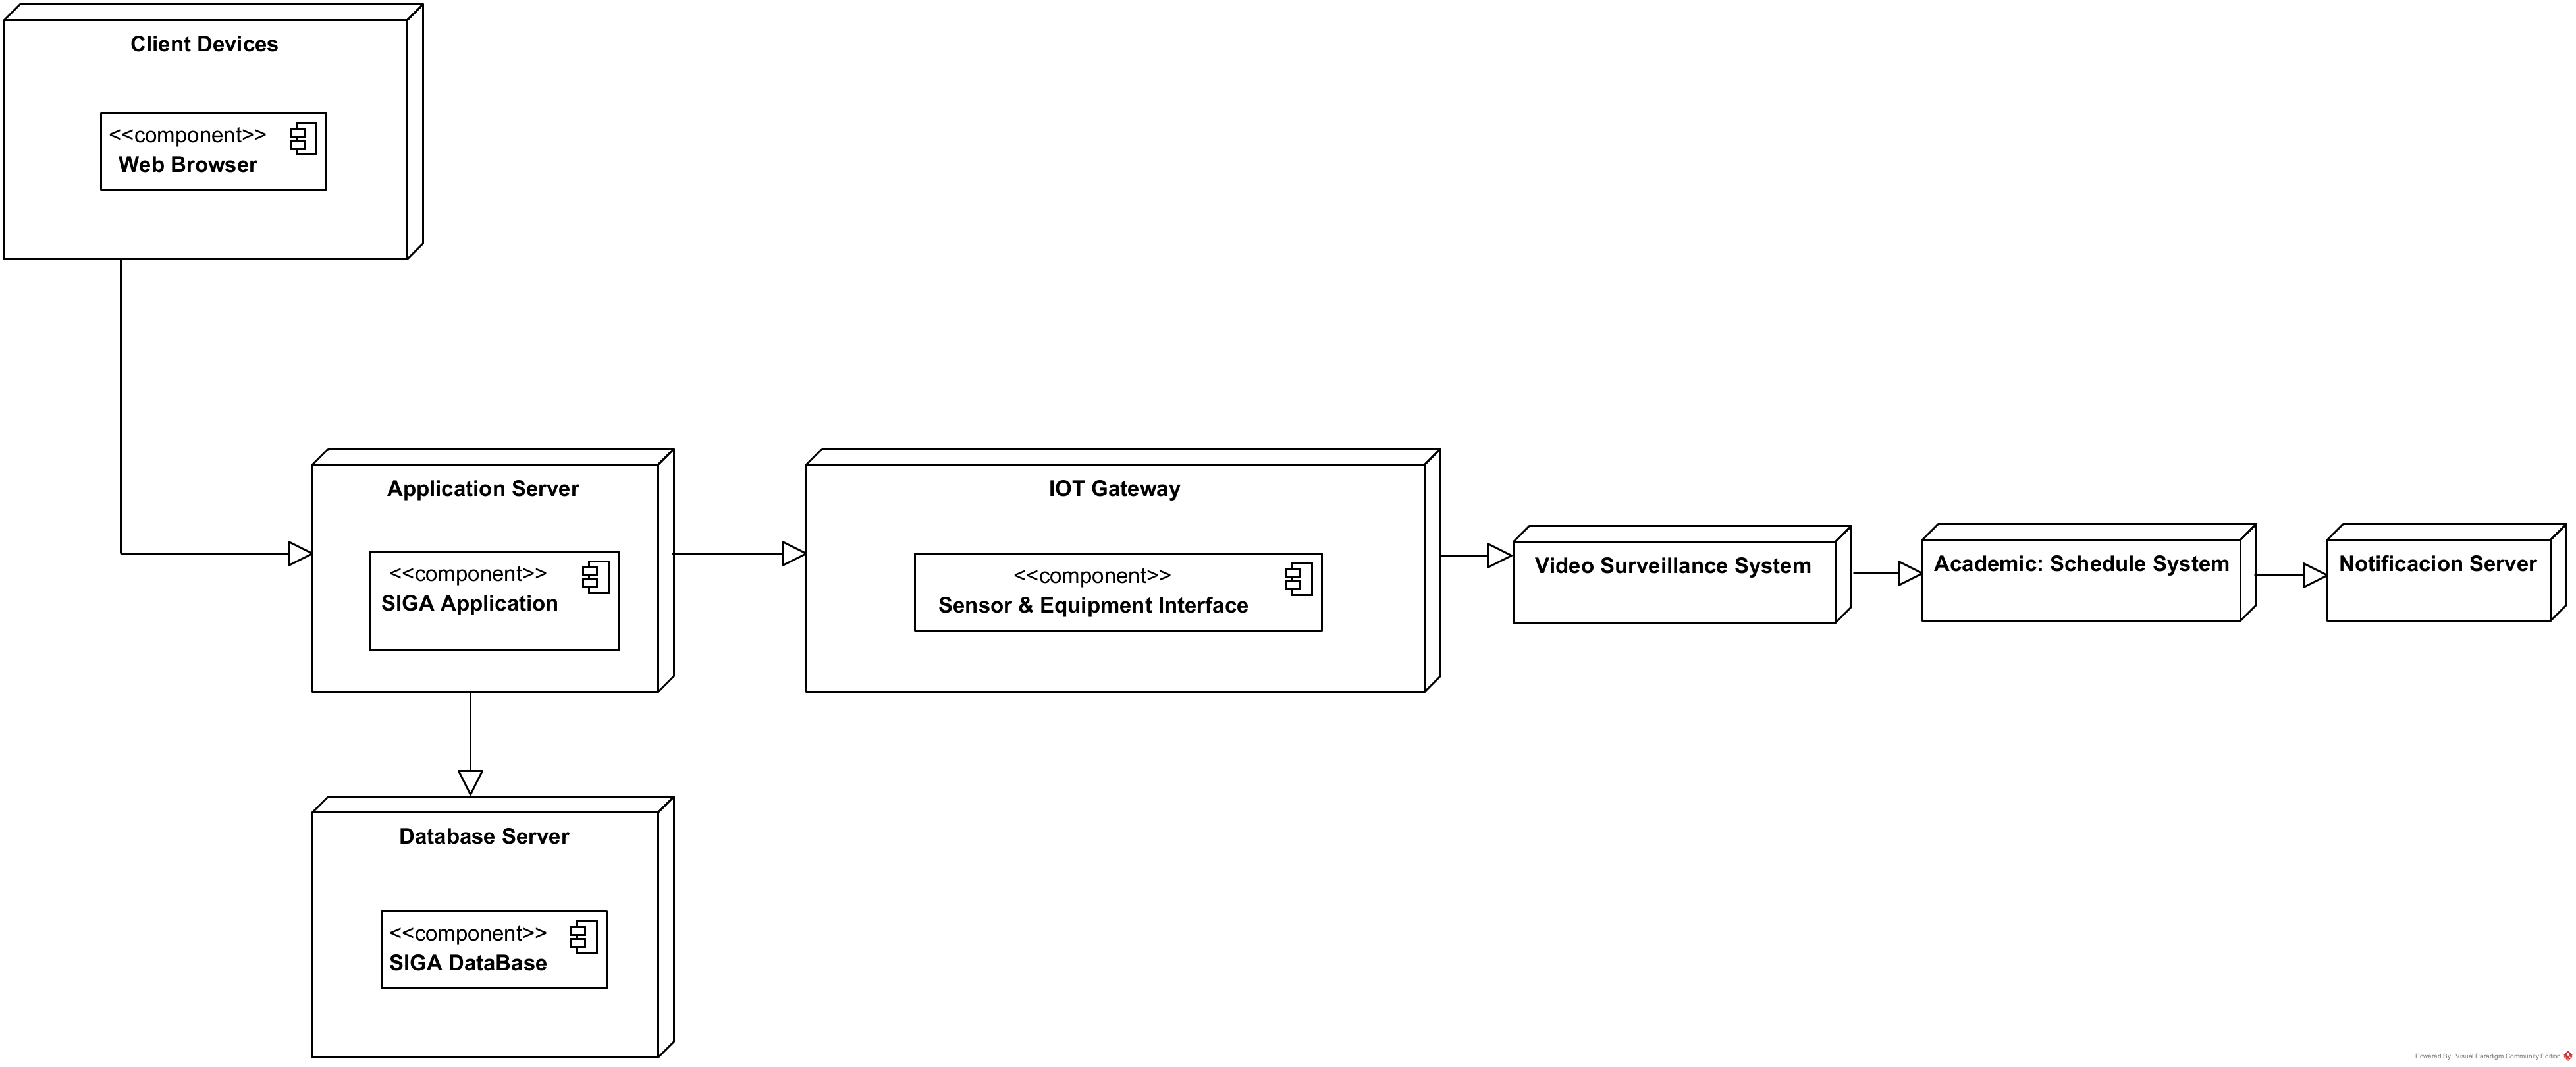
\includegraphics[width=0.85\textwidth,height=0.8\textheight,keepaspectratio]{figuras/deployment_diagram.png}
\caption{Diagrama de despliegue --- SIGA}
\label{fig:img17}
\end{figure}

\subsection*{4.9 Diagramas de secuencia y actividad complementarios (CU-01 a CU-16)}

\addcontentsline{toc}{subsection}{4.9 Diagramas de secuencia y actividad complementarios (CU-01 a CU-16)}

Se presentan a continuación los diagramas de secuencia y de actividad individuales para los 16 casos de uso, elaborados en Visual Paradigm (archivo fuente editable \texttt{.vpp} conservado en el repositorio, conforme a la decisión del equipo de no exportar a XMI). Los diagramas de CU-04 y CU-06 ya presentados en las secciones 4.5/4.6 como flujo narrativo se incluyen aquí también en su forma gráfica completa para mantener consistencia con el resto del conjunto.

\begin{figure}[H]
\centering
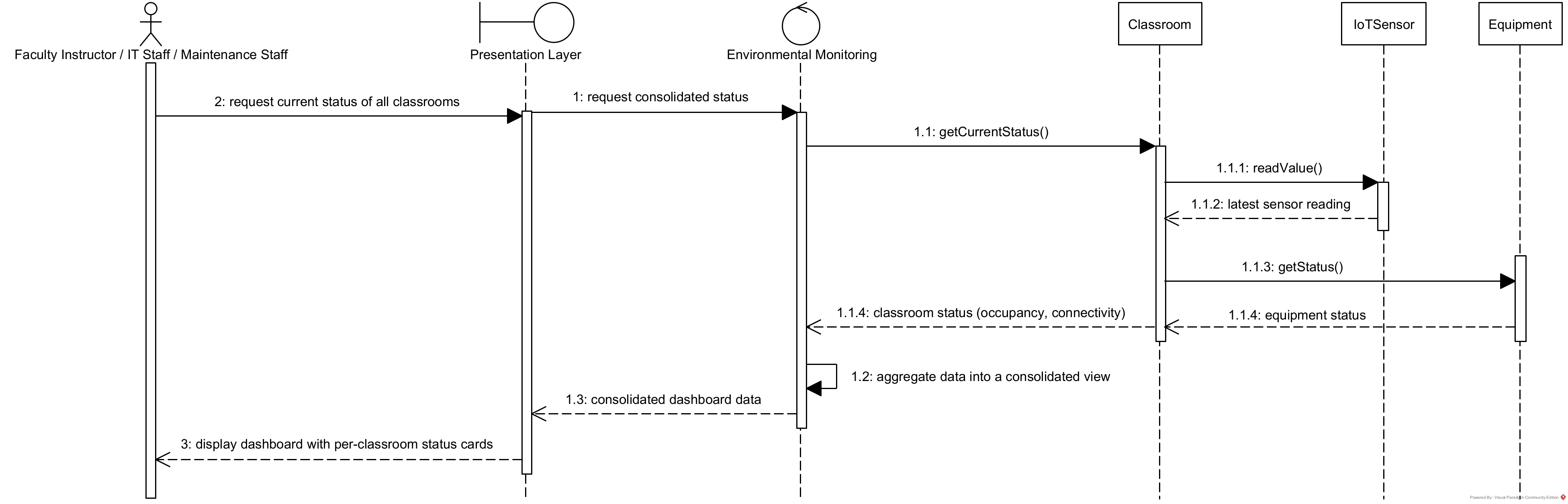
\includegraphics[width=0.85\textwidth,height=0.8\textheight,keepaspectratio]{figuras/seq_UC01_monitor_room_status.png}
\caption{Diagrama de secuencia --- CU-01 Monitorear estado de aula en tiempo real}
\label{fig:seq-cu01}
\end{figure}

\begin{figure}[H]
\centering
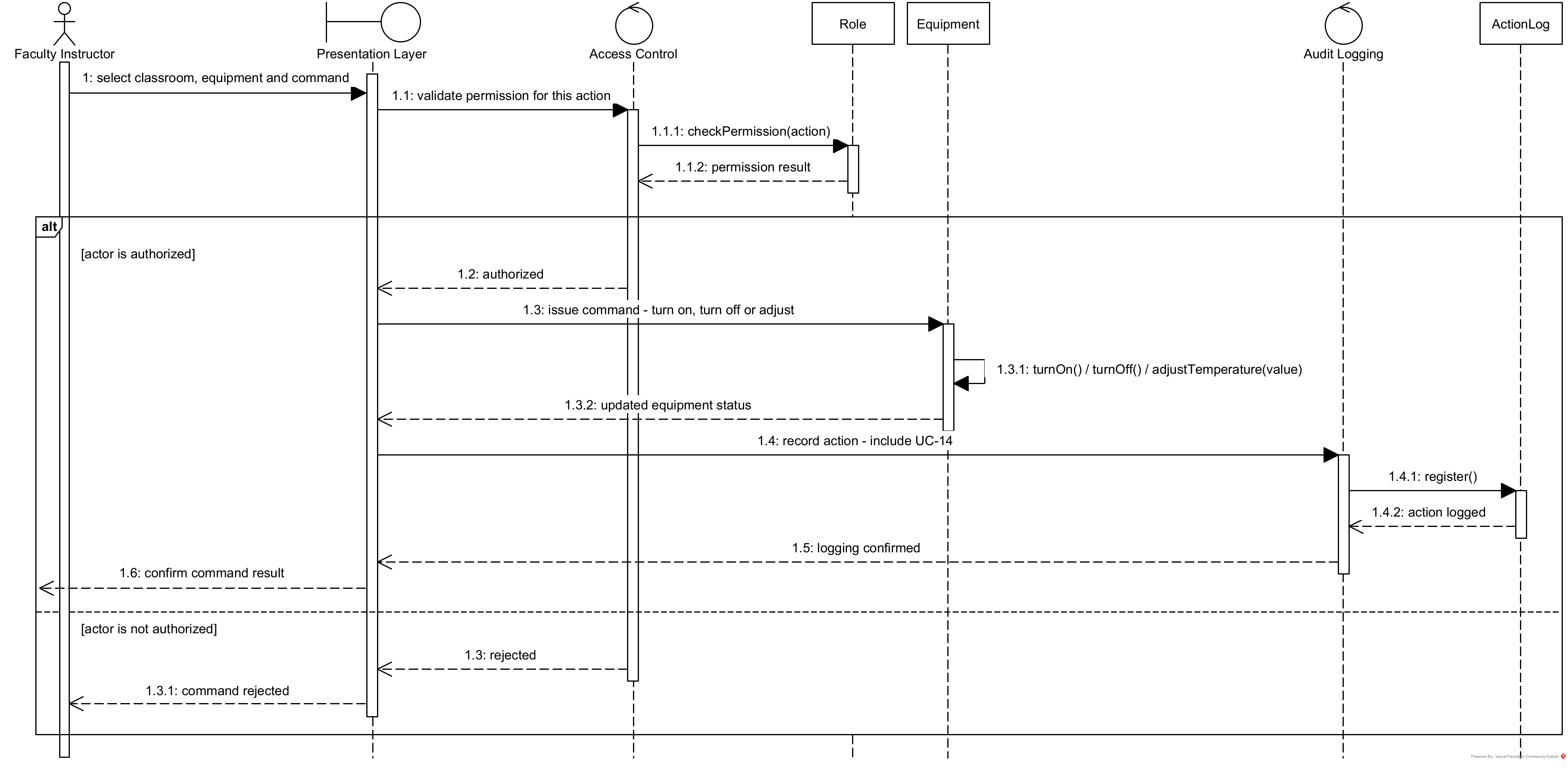
\includegraphics[width=0.85\textwidth,height=0.8\textheight,keepaspectratio]{figuras/seq_UC02_remote_equipment_control.png}
\caption{Diagrama de secuencia --- CU-02 Controlar remotamente equipos de aula}
\label{fig:seq-cu02}
\end{figure}

\begin{figure}[H]
\centering
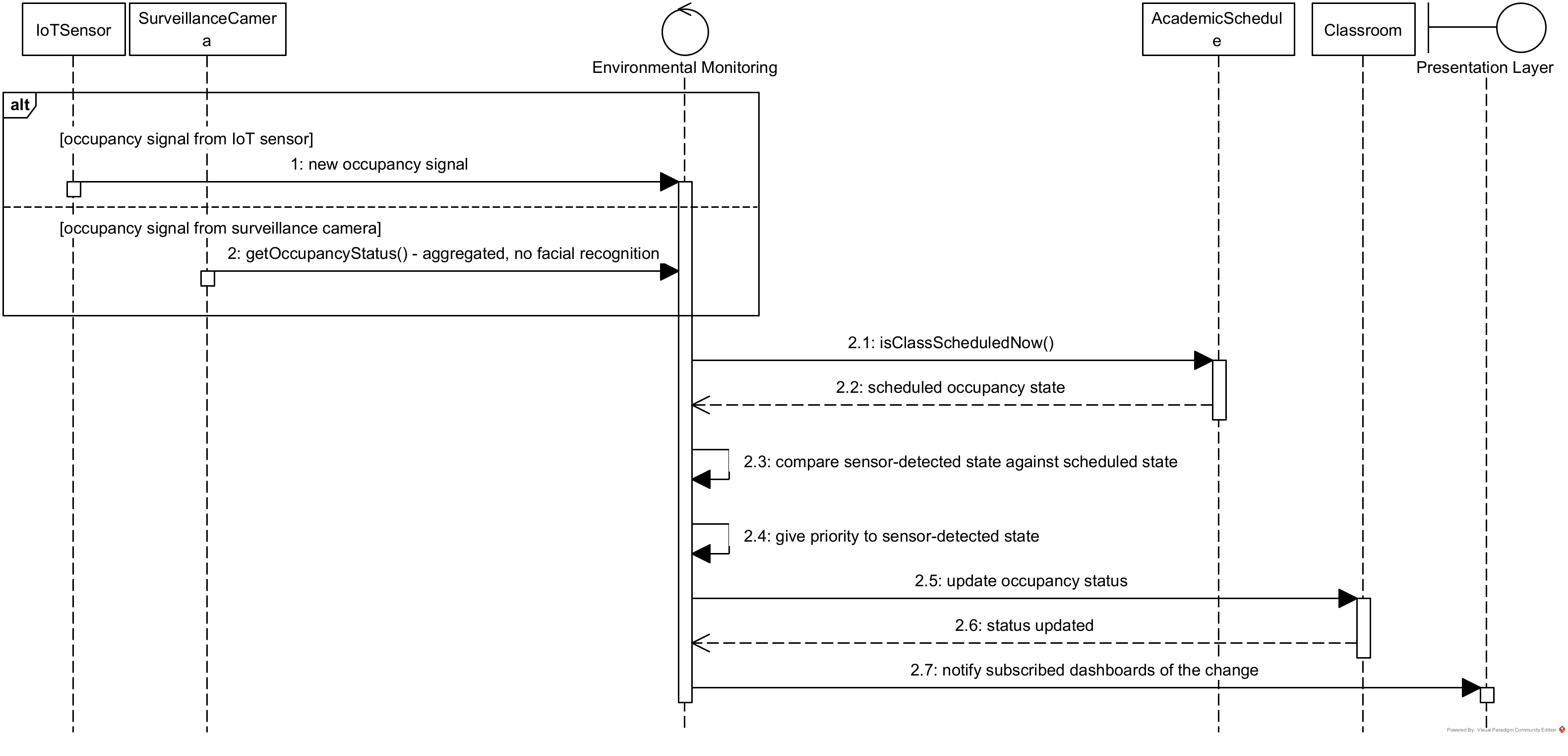
\includegraphics[width=0.85\textwidth,height=0.8\textheight,keepaspectratio]{figuras/seq_UC03_detect_room_occupancy.png}
\caption{Diagrama de secuencia --- CU-03 Detectar ocupación de aula}
\label{fig:seq-cu03}
\end{figure}

\begin{figure}[H]
\centering
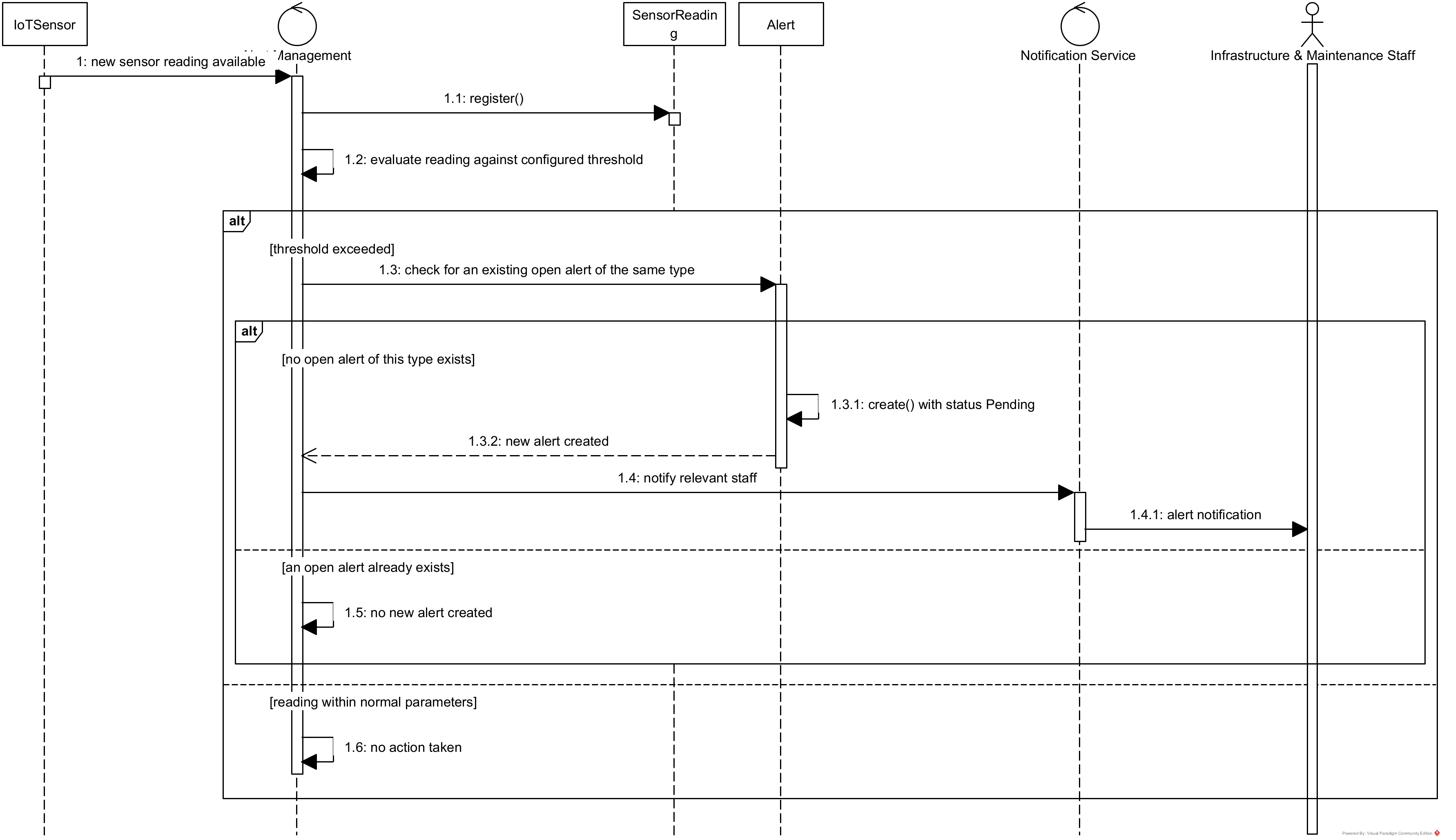
\includegraphics[width=0.85\textwidth,height=0.8\textheight,keepaspectratio]{figuras/seq_UC04_generate_anomaly_alerts.png}
\caption{Diagrama de secuencia --- CU-04 Generar alertas por anomalías}
\label{fig:seq-cu04}
\end{figure}

\begin{figure}[H]
\centering
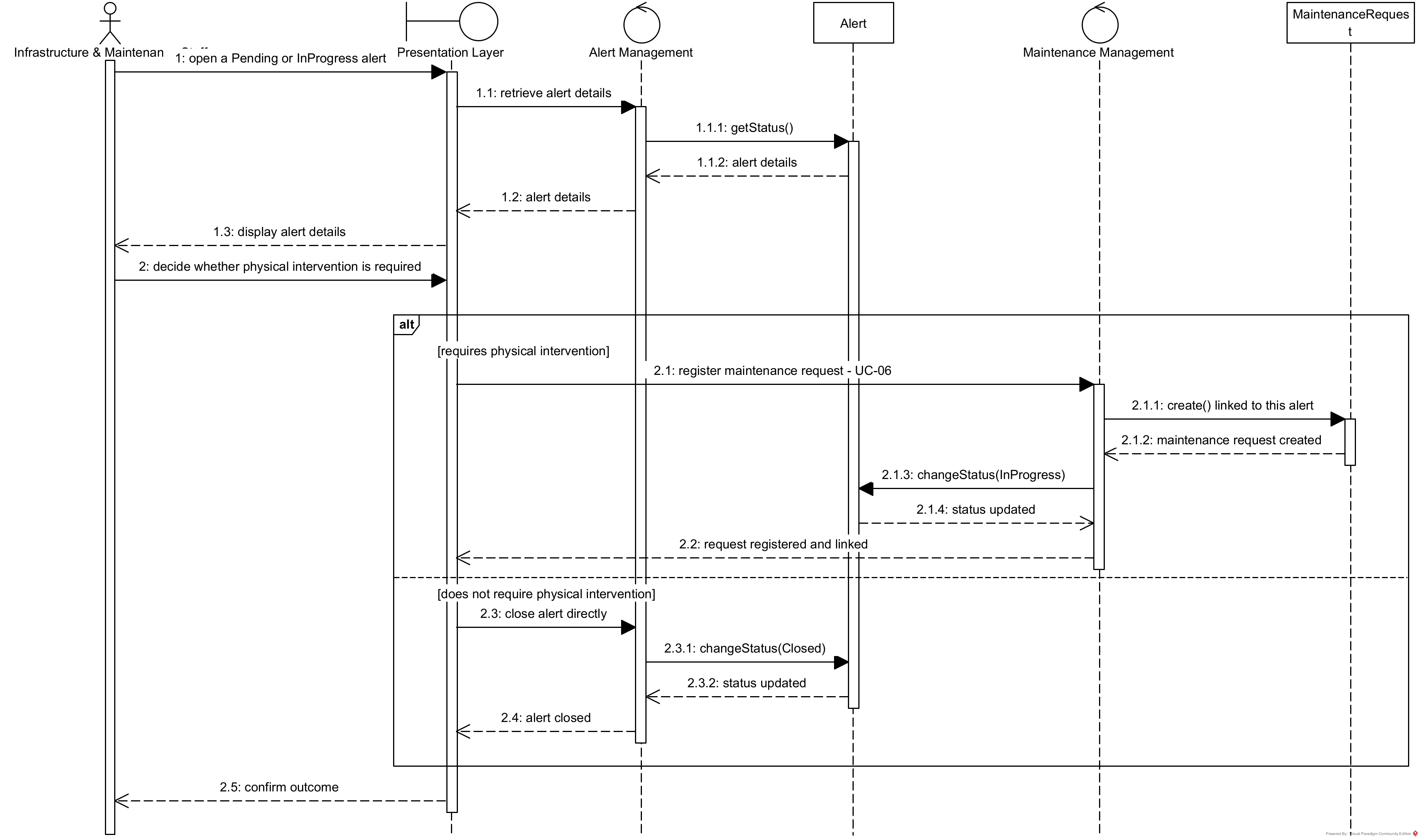
\includegraphics[width=0.85\textwidth,height=0.8\textheight,keepaspectratio]{figuras/seq_UC05_attend_anomaly_alert.png}
\caption{Diagrama de secuencia --- CU-05 Atender alerta de anomalía}
\label{fig:seq-cu05}
\end{figure}

\begin{figure}[H]
\centering
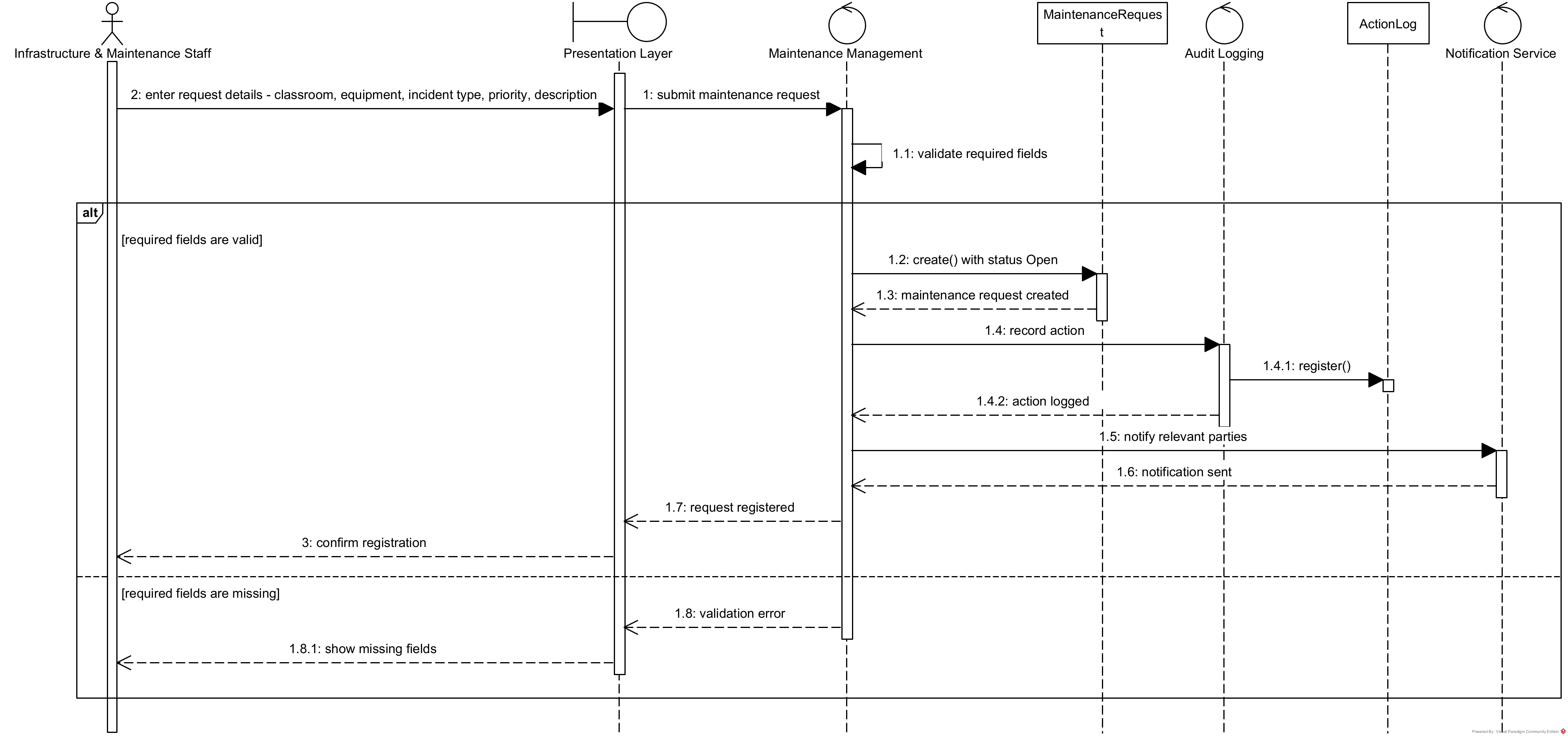
\includegraphics[width=0.85\textwidth,height=0.8\textheight,keepaspectratio]{figuras/seq_UC06_register_maintenance_request.png}
\caption{Diagrama de secuencia --- CU-06 Registrar solicitud de mantenimiento}
\label{fig:seq-cu06}
\end{figure}

\begin{figure}[H]
\centering
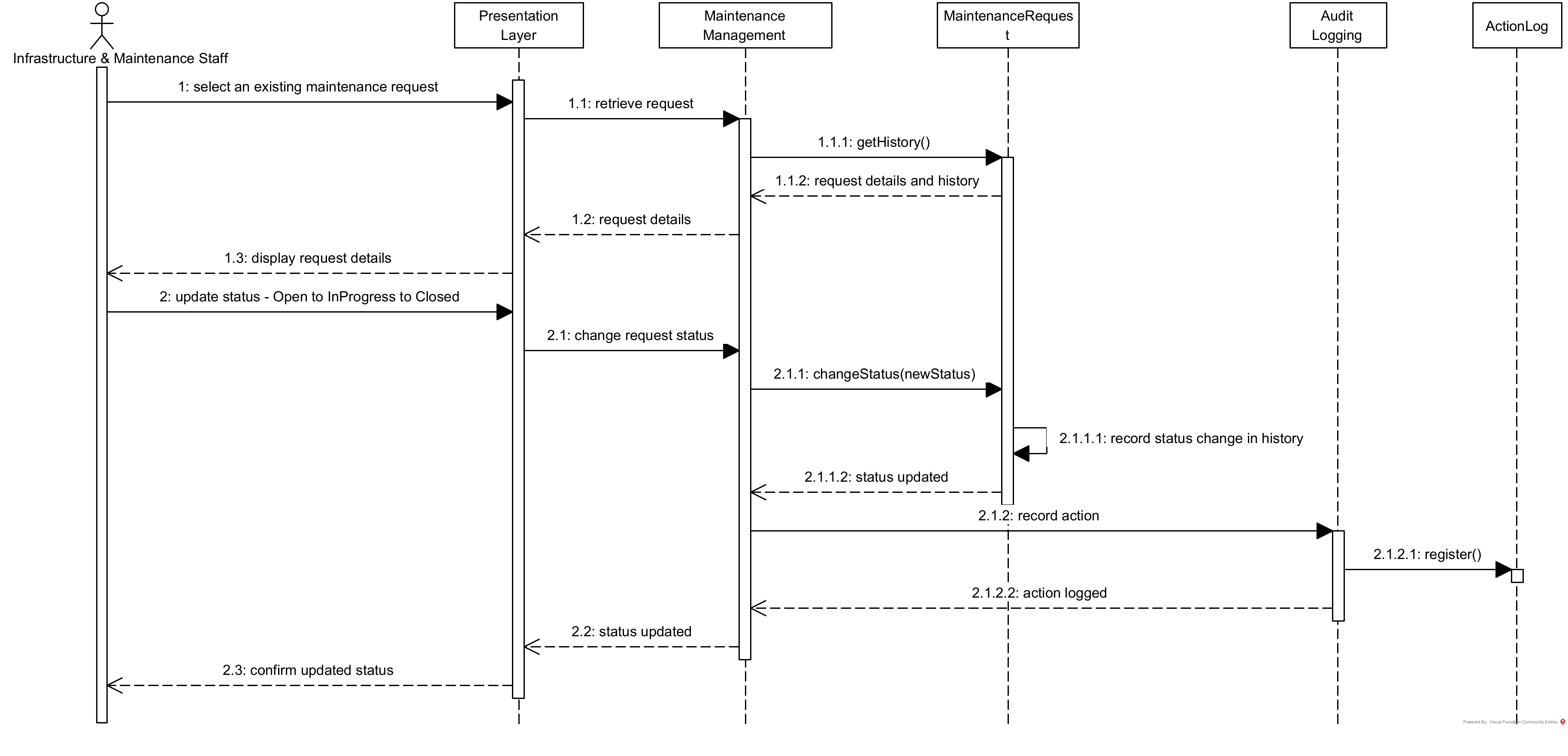
\includegraphics[width=0.85\textwidth,height=0.8\textheight,keepaspectratio]{figuras/seq_UC07_track_maintenance_ticket.png}
\caption{Diagrama de secuencia --- CU-07 Dar seguimiento a ticket de mantenimiento}
\label{fig:seq-cu07}
\end{figure}

\begin{figure}[H]
\centering
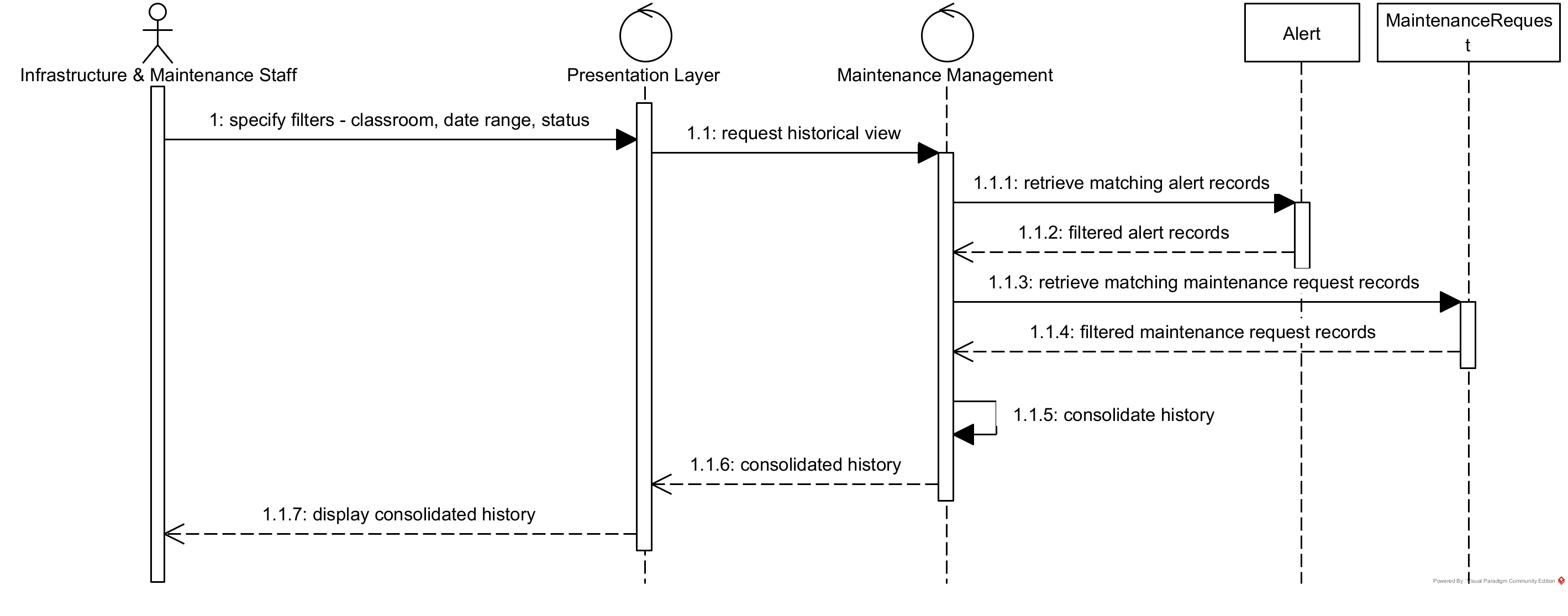
\includegraphics[width=0.85\textwidth,height=0.8\textheight,keepaspectratio]{figuras/seq_UC08_view_failure_maintenance_history.png}
\caption{Diagrama de secuencia --- CU-08 Consultar historial de fallas y mantenimientos}
\label{fig:seq-cu08}
\end{figure}

\begin{figure}[H]
\centering
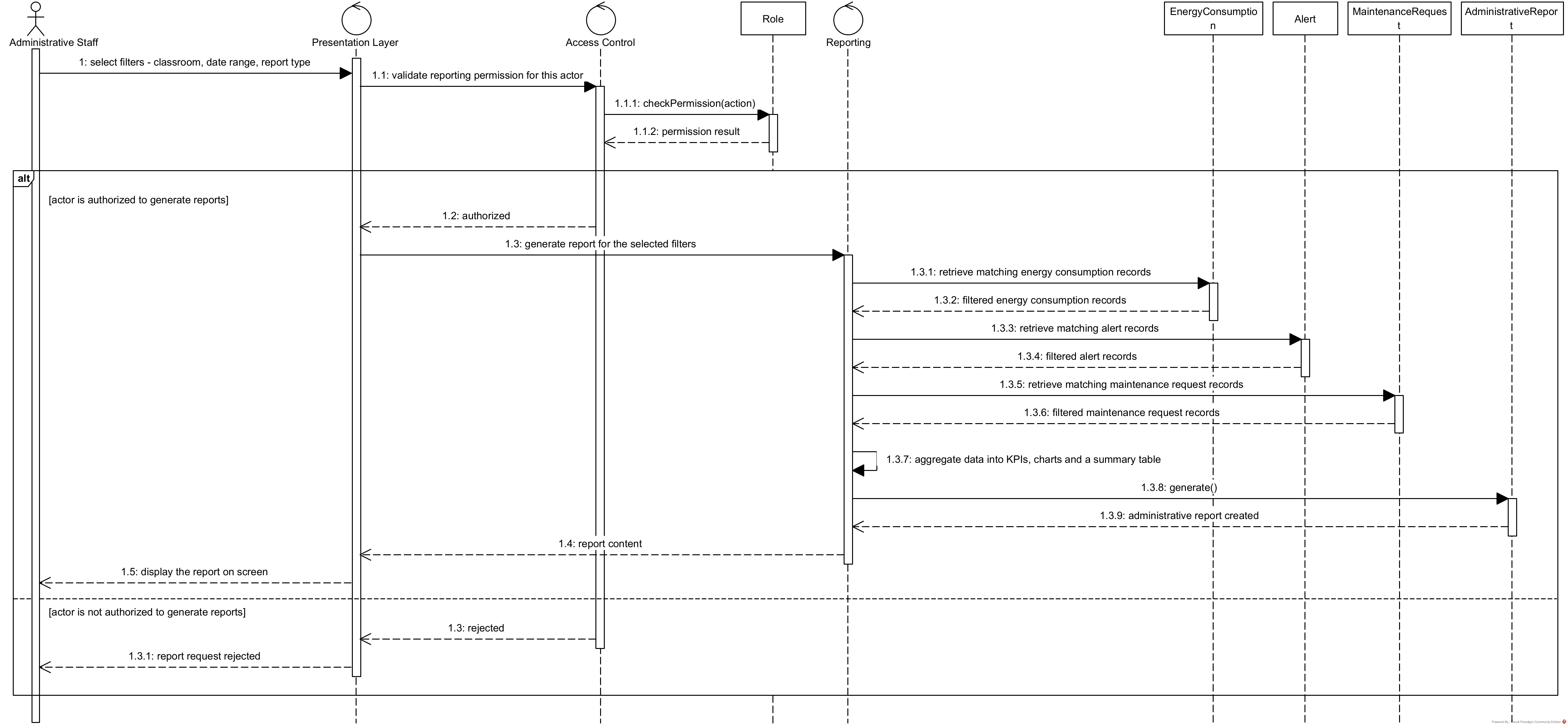
\includegraphics[width=0.85\textwidth,height=0.8\textheight,keepaspectratio]{figuras/seq_UC09_generate_administrative_reports.png}
\caption{Diagrama de secuencia --- CU-09 Generar reportes administrativos}
\label{fig:seq-cu09}
\end{figure}

\begin{figure}[H]
\centering
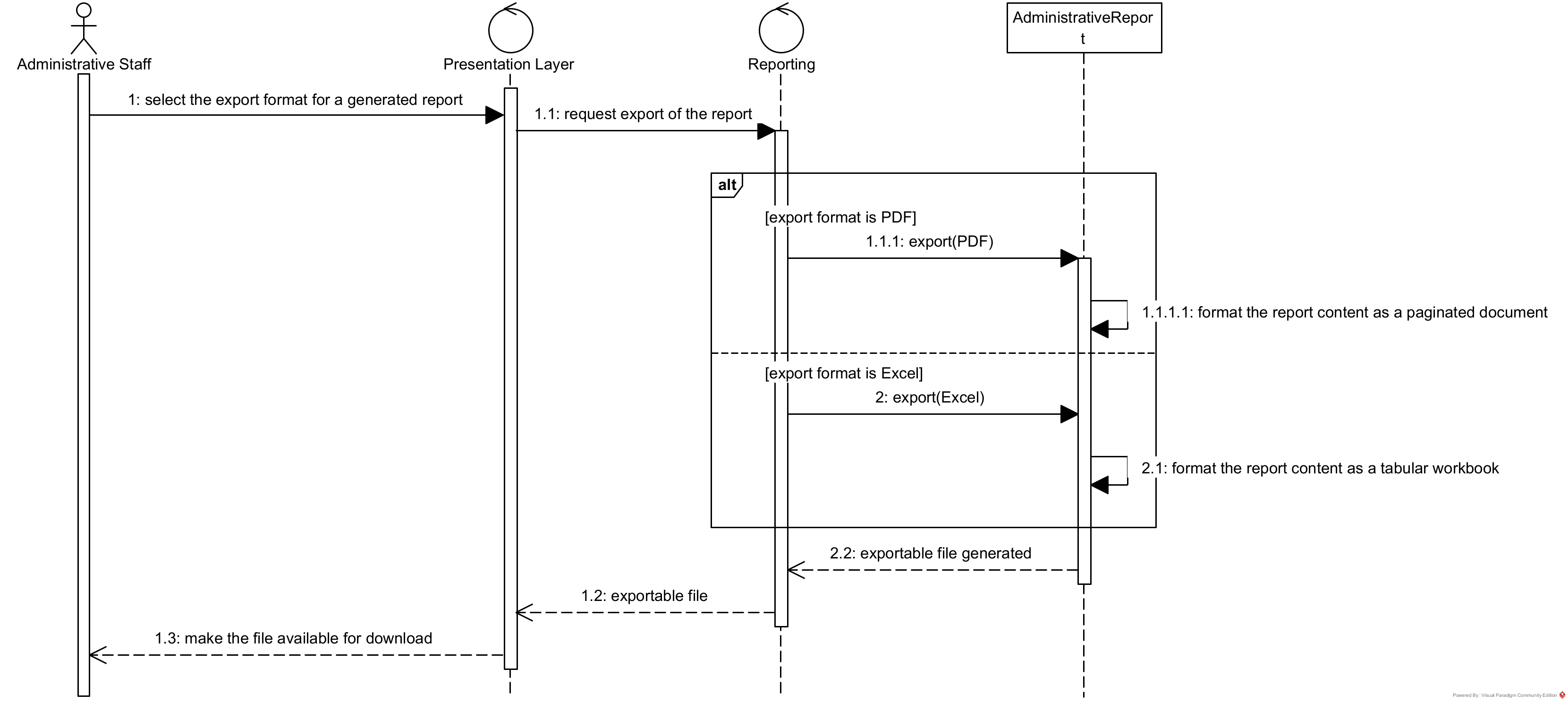
\includegraphics[width=0.85\textwidth,height=0.8\textheight,keepaspectratio]{figuras/seq_UC10_export_reports.png}
\caption{Diagrama de secuencia --- CU-10 Exportar reportes PDF y Excel}
\label{fig:seq-cu10}
\end{figure}

\begin{figure}[H]
\centering
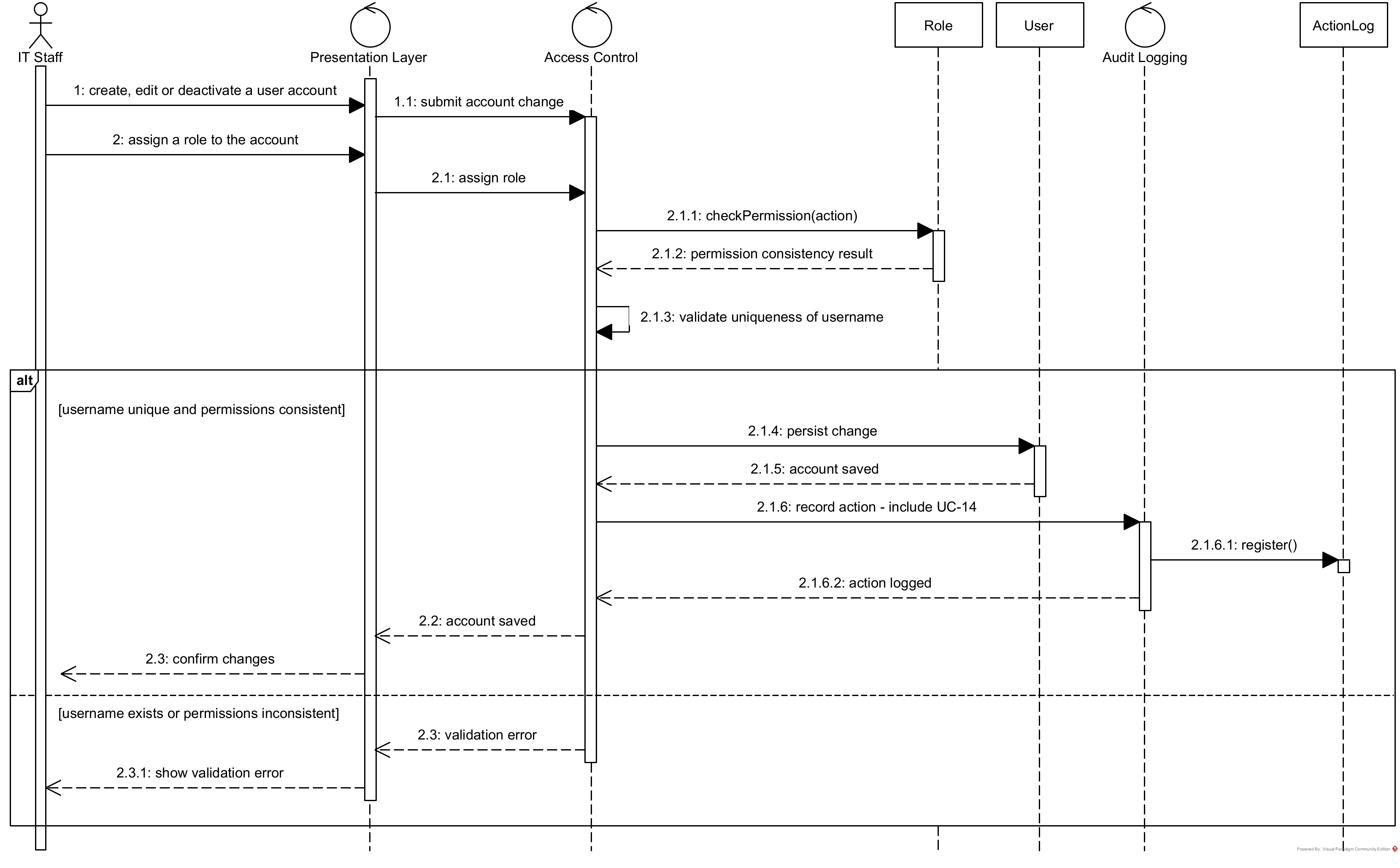
\includegraphics[width=0.85\textwidth,height=0.8\textheight,keepaspectratio]{figuras/seq_UC11_manage_users_roles_permissions.png}
\caption{Diagrama de secuencia --- CU-11 Gestionar usuarios, roles y permisos}
\label{fig:seq-cu11}
\end{figure}

\begin{figure}[H]
\centering
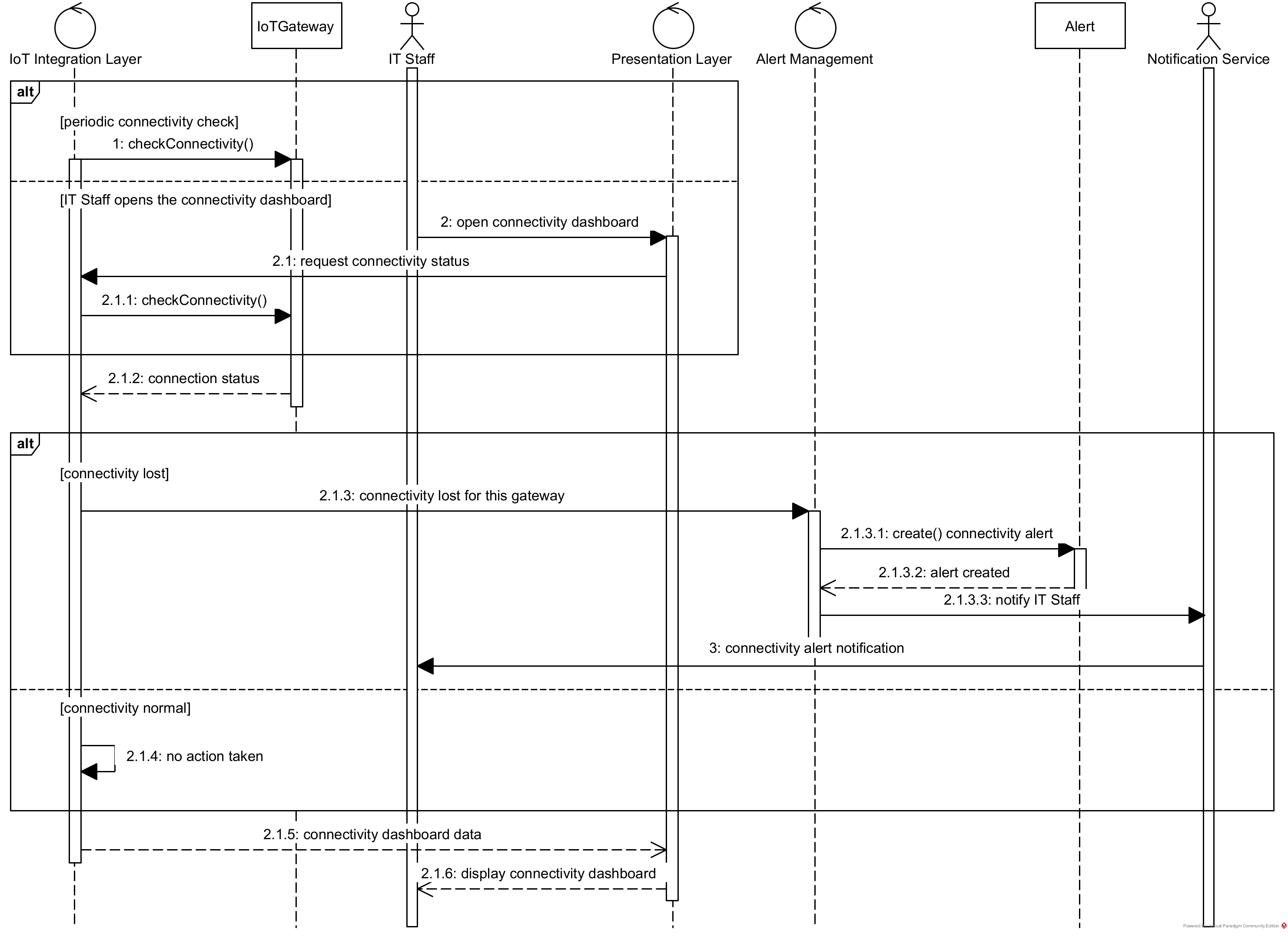
\includegraphics[width=0.85\textwidth,height=0.8\textheight,keepaspectratio]{figuras/seq_UC12_monitor_iot_connectivity.png}
\caption{Diagrama de secuencia --- CU-12 Monitorear conectividad IoT}
\label{fig:seq-cu12}
\end{figure}

\begin{figure}[H]
\centering
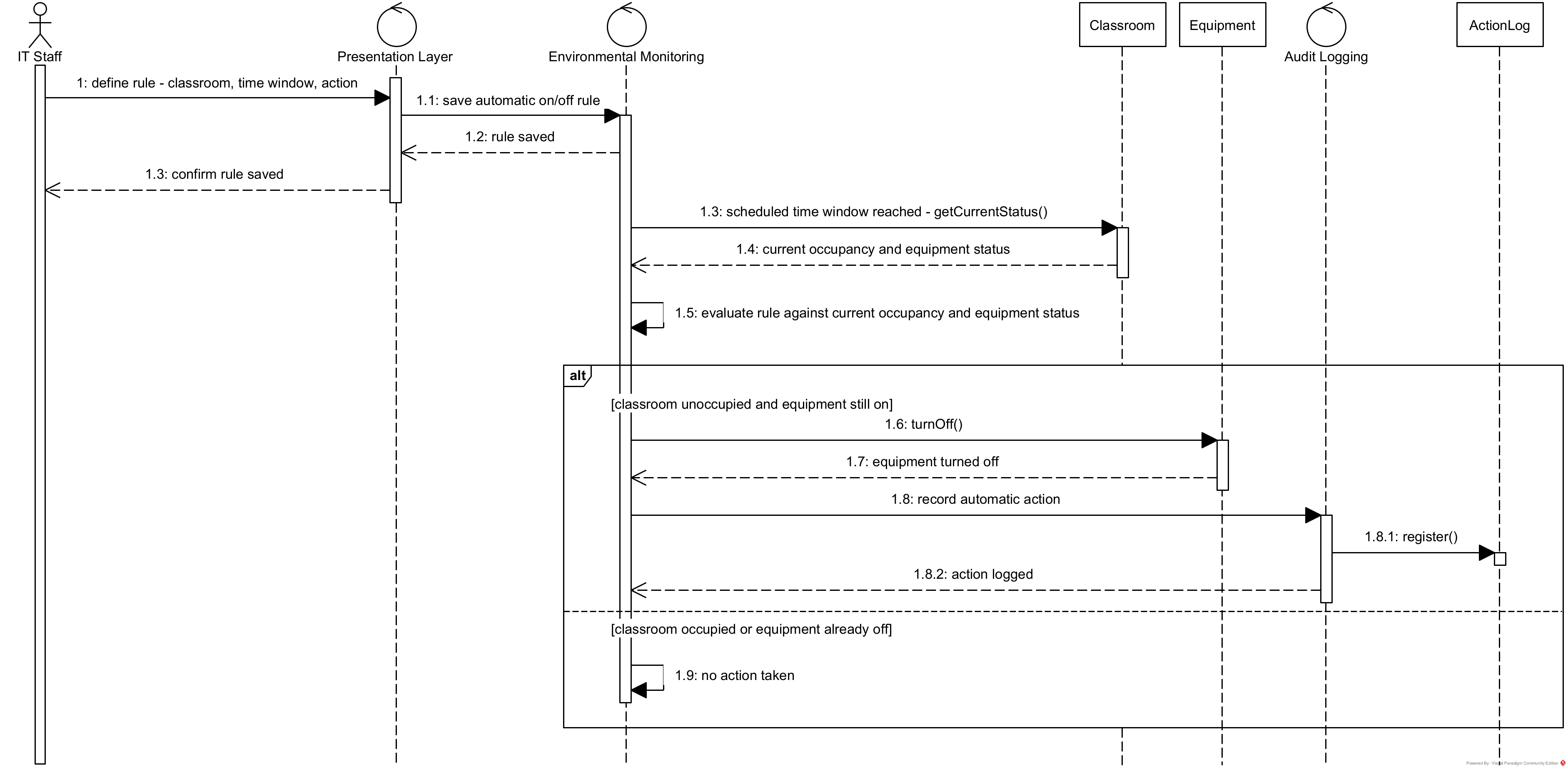
\includegraphics[width=0.85\textwidth,height=0.8\textheight,keepaspectratio]{figuras/seq_UC13_schedule_automatic_onoff_rules.png}
\caption{Diagrama de secuencia --- CU-13 Programar reglas de encendido y apagado}
\label{fig:seq-cu13}
\end{figure}

\begin{figure}[H]
\centering
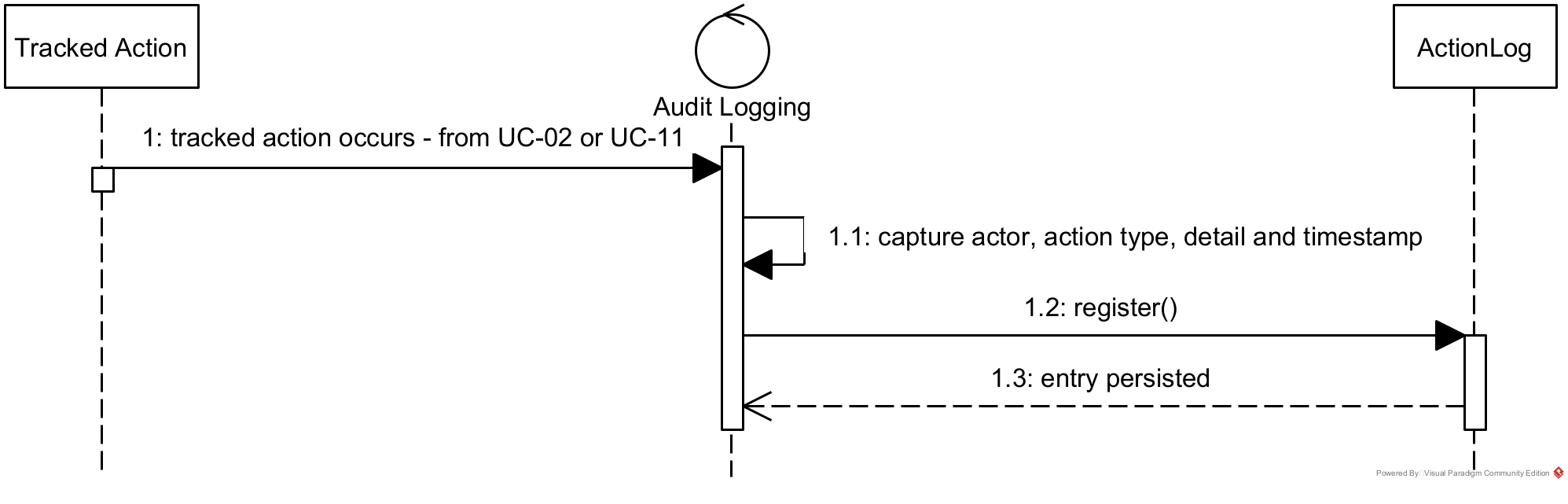
\includegraphics[width=0.85\textwidth,height=0.8\textheight,keepaspectratio]{figuras/seq_UC14_log_user_actions.png}
\caption{Diagrama de secuencia --- CU-14 Registrar bitácora de acciones}
\label{fig:seq-cu14}
\end{figure}

\begin{figure}[H]
\centering
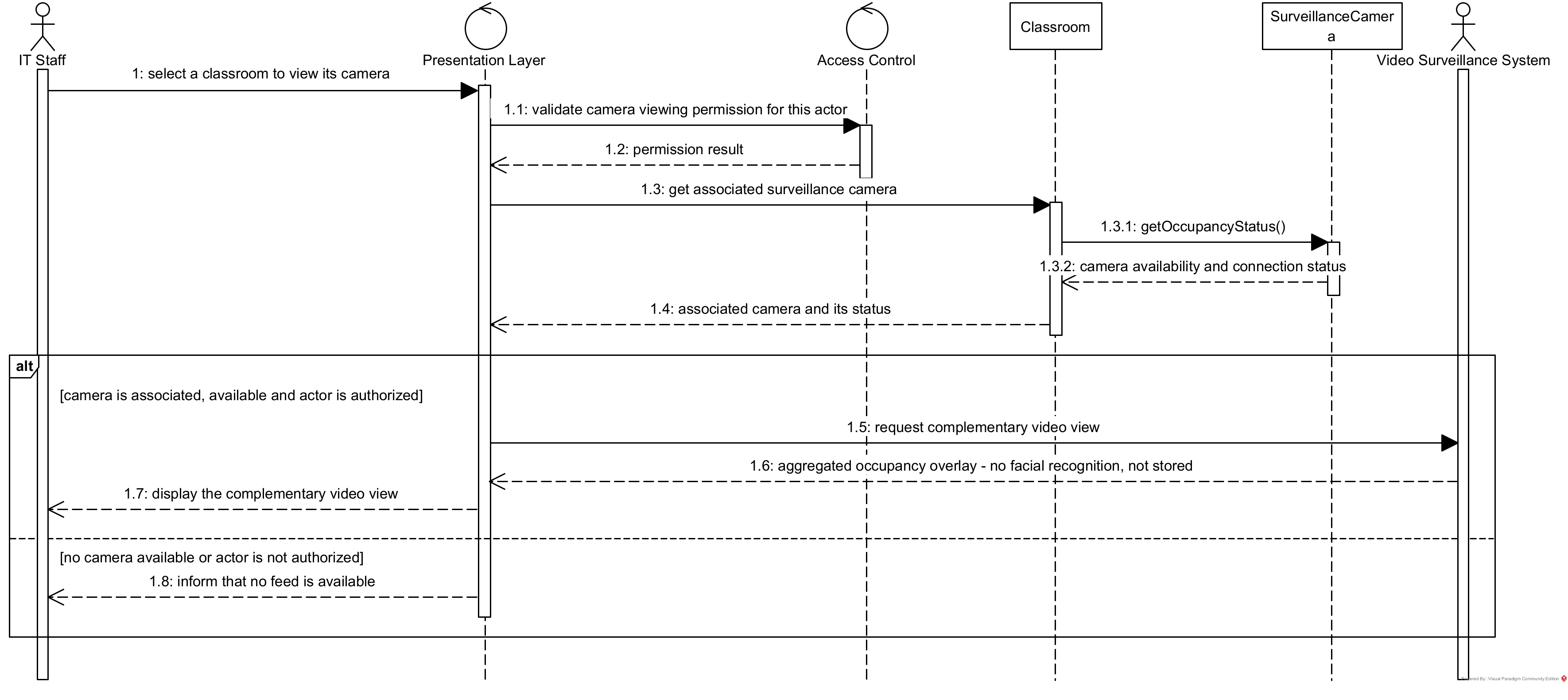
\includegraphics[width=0.85\textwidth,height=0.8\textheight,keepaspectratio]{figuras/seq_UC15_view_room_cameras.png}
\caption{Diagrama de secuencia --- CU-15 Consultar cámaras asociadas al aula}
\label{fig:seq-cu15}
\end{figure}

\begin{figure}[H]
\centering
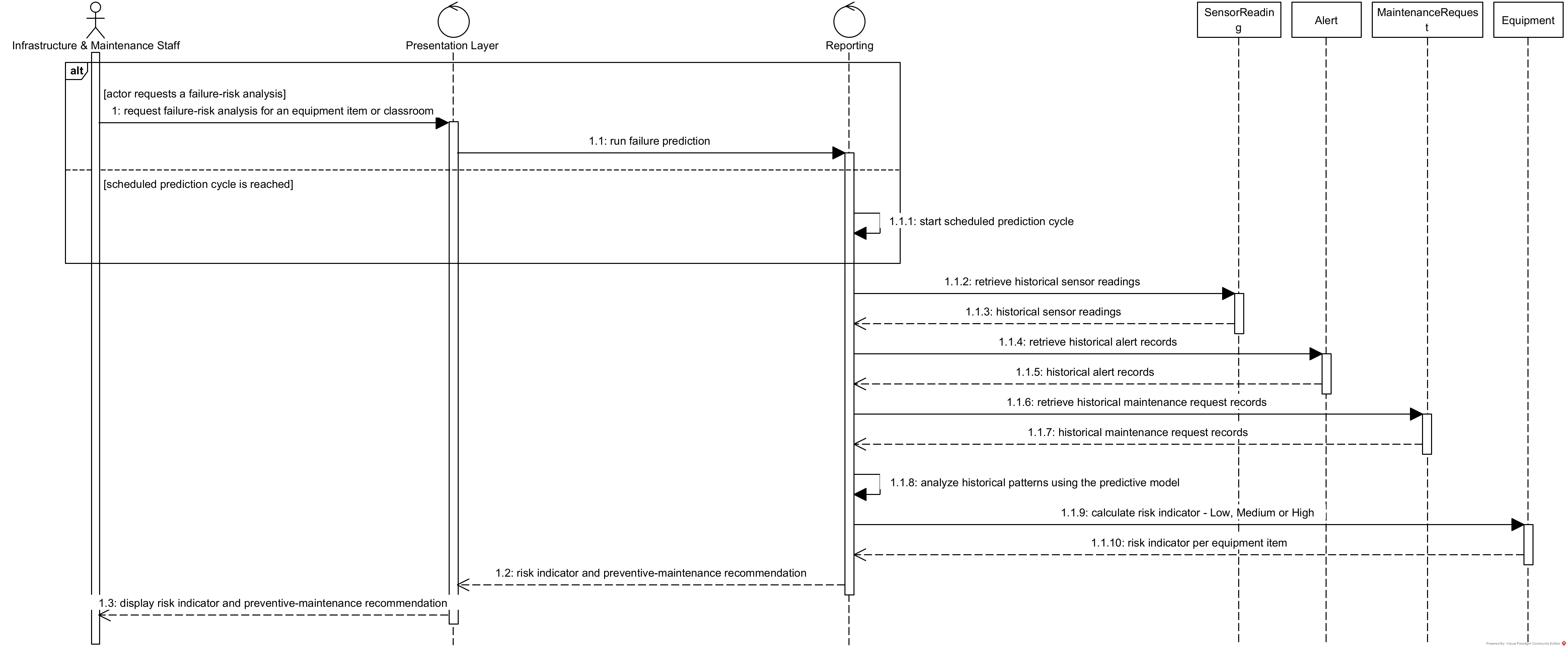
\includegraphics[width=0.85\textwidth,height=0.8\textheight,keepaspectratio]{figuras/seq_UC16_predict_equipment_failures.png}
\caption{Diagrama de secuencia --- CU-16 Predecir fallas de equipos}
\label{fig:seq-cu16}
\end{figure}

\begin{figure}[H]
\centering
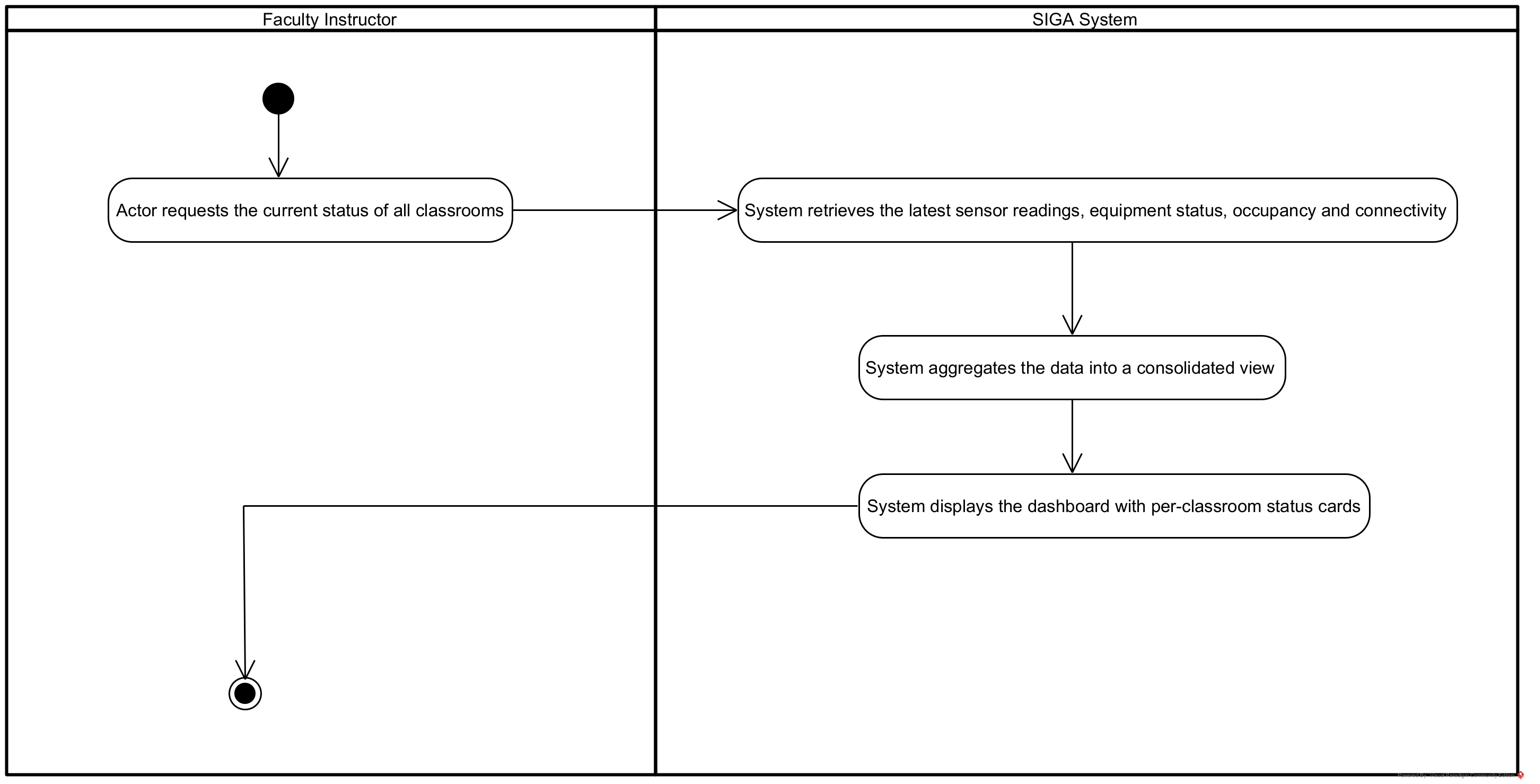
\includegraphics[width=0.85\textwidth,height=0.8\textheight,keepaspectratio]{figuras/act_UC01_monitor_room_status.png}
\caption{Diagrama de actividad --- CU-01 Monitorear estado de aula en tiempo real}
\label{fig:act-cu01}
\end{figure}

\begin{figure}[H]
\centering
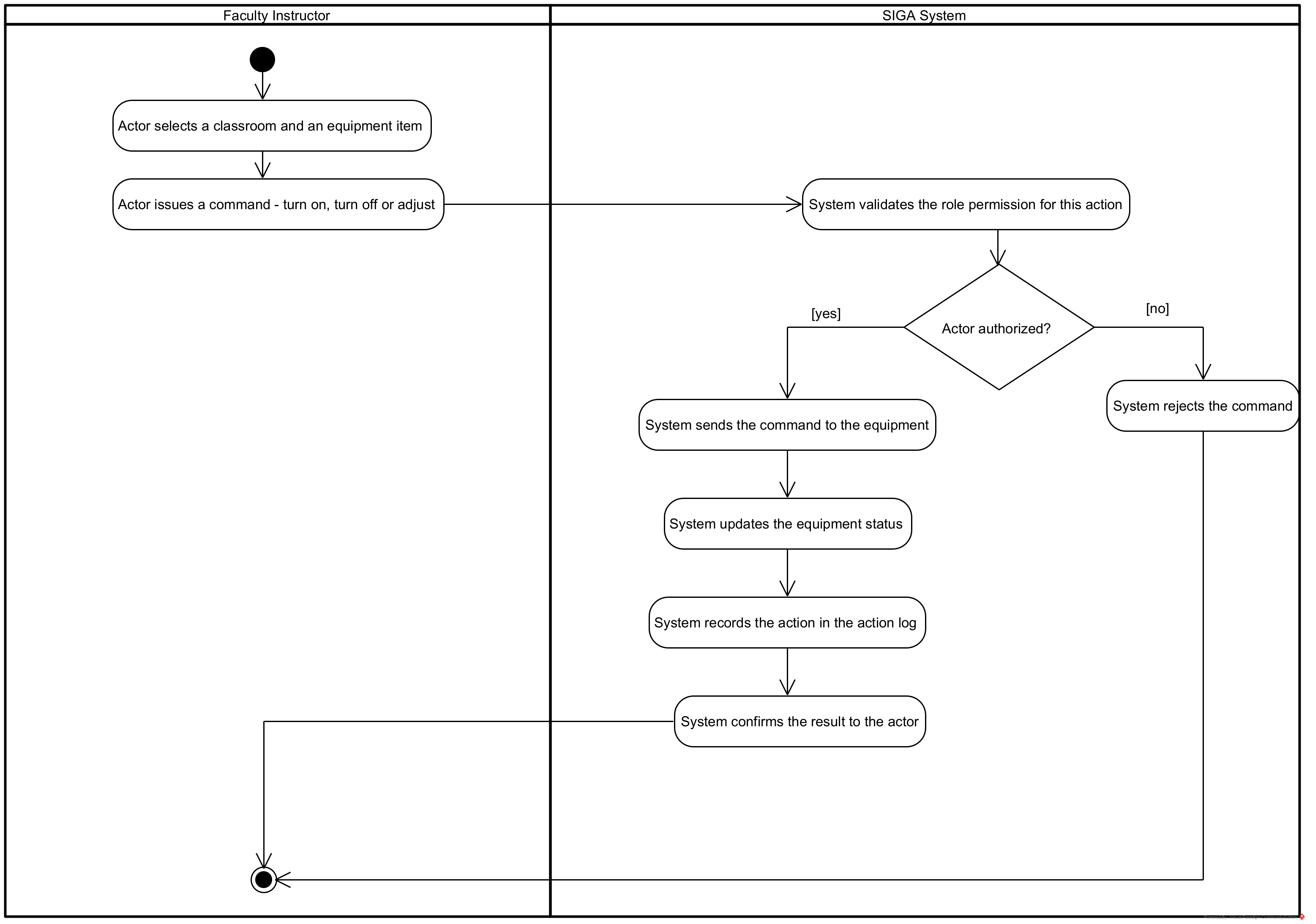
\includegraphics[width=0.85\textwidth,height=0.8\textheight,keepaspectratio]{figuras/act_UC02_remote_equipment_control.png}
\caption{Diagrama de actividad --- CU-02 Controlar remotamente equipos de aula}
\label{fig:act-cu02}
\end{figure}

\begin{figure}[H]
\centering
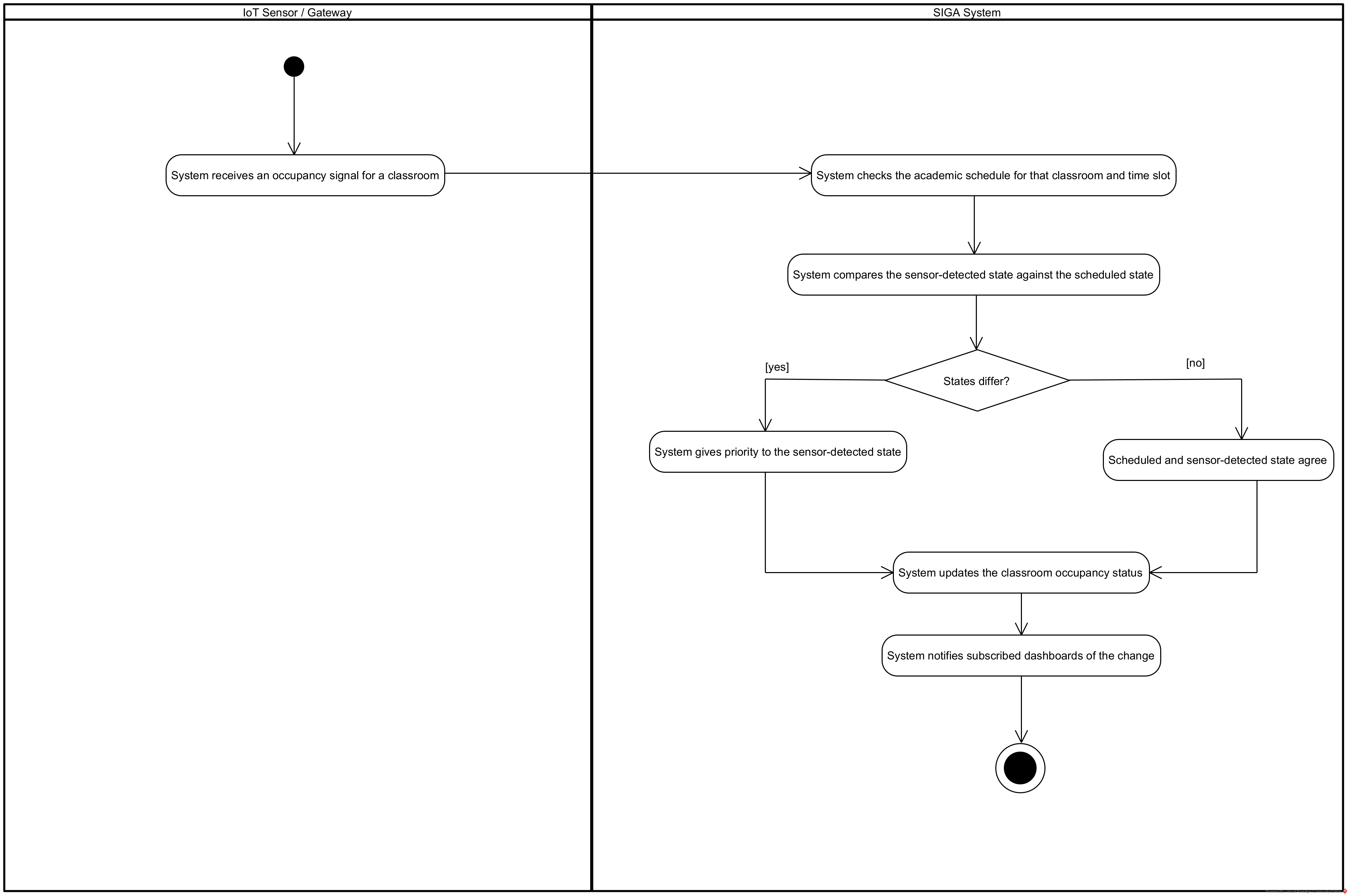
\includegraphics[width=0.85\textwidth,height=0.8\textheight,keepaspectratio]{figuras/act_UC03_detect_room_occupancy.png}
\caption{Diagrama de actividad --- CU-03 Detectar ocupación de aula}
\label{fig:act-cu03}
\end{figure}

\begin{figure}[H]
\centering
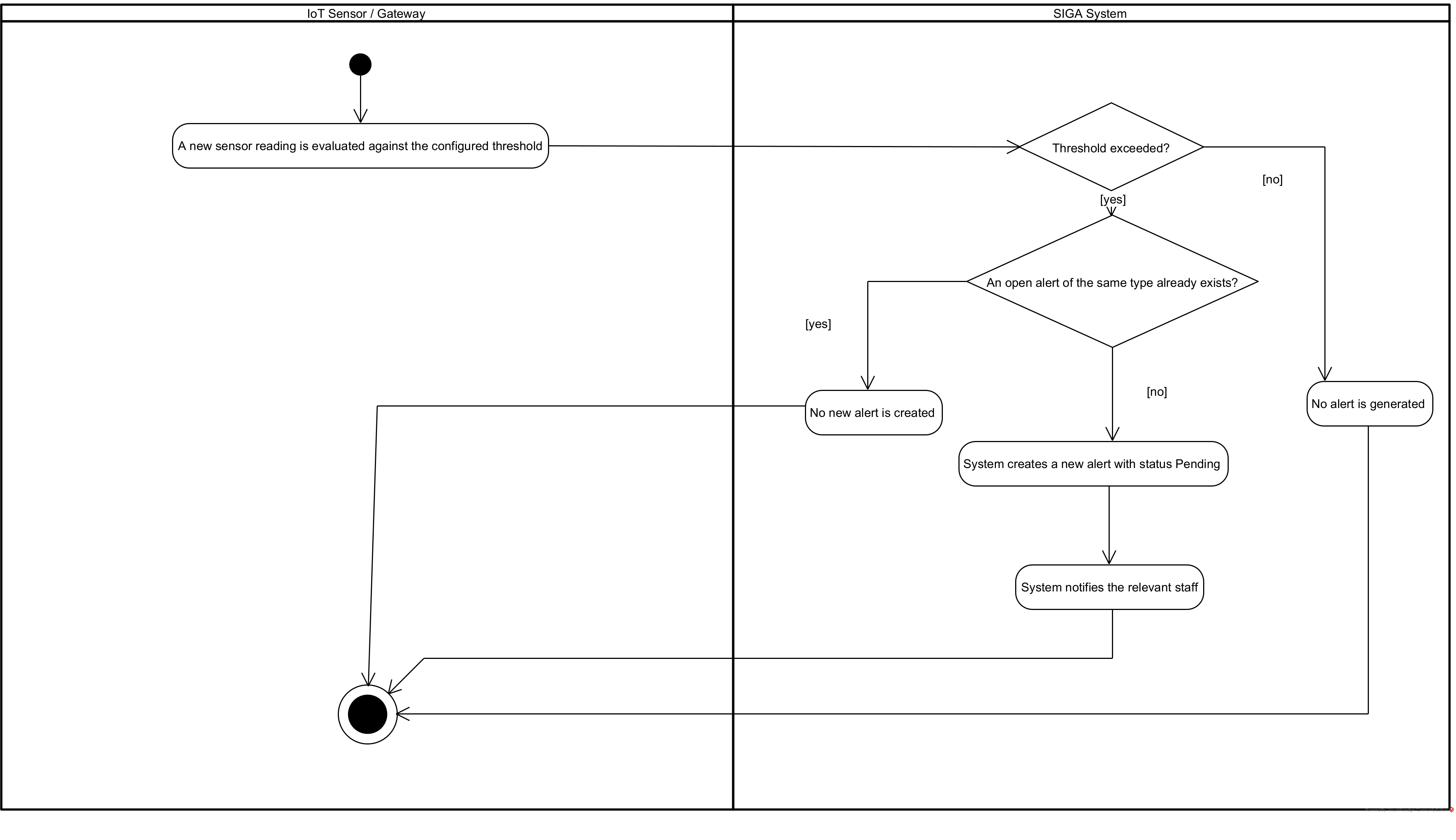
\includegraphics[width=0.85\textwidth,height=0.8\textheight,keepaspectratio]{figuras/act_UC04_generate_anomaly_alerts.png}
\caption{Diagrama de actividad --- CU-04 Generar alertas por anomalías}
\label{fig:act-cu04}
\end{figure}

\begin{figure}[H]
\centering
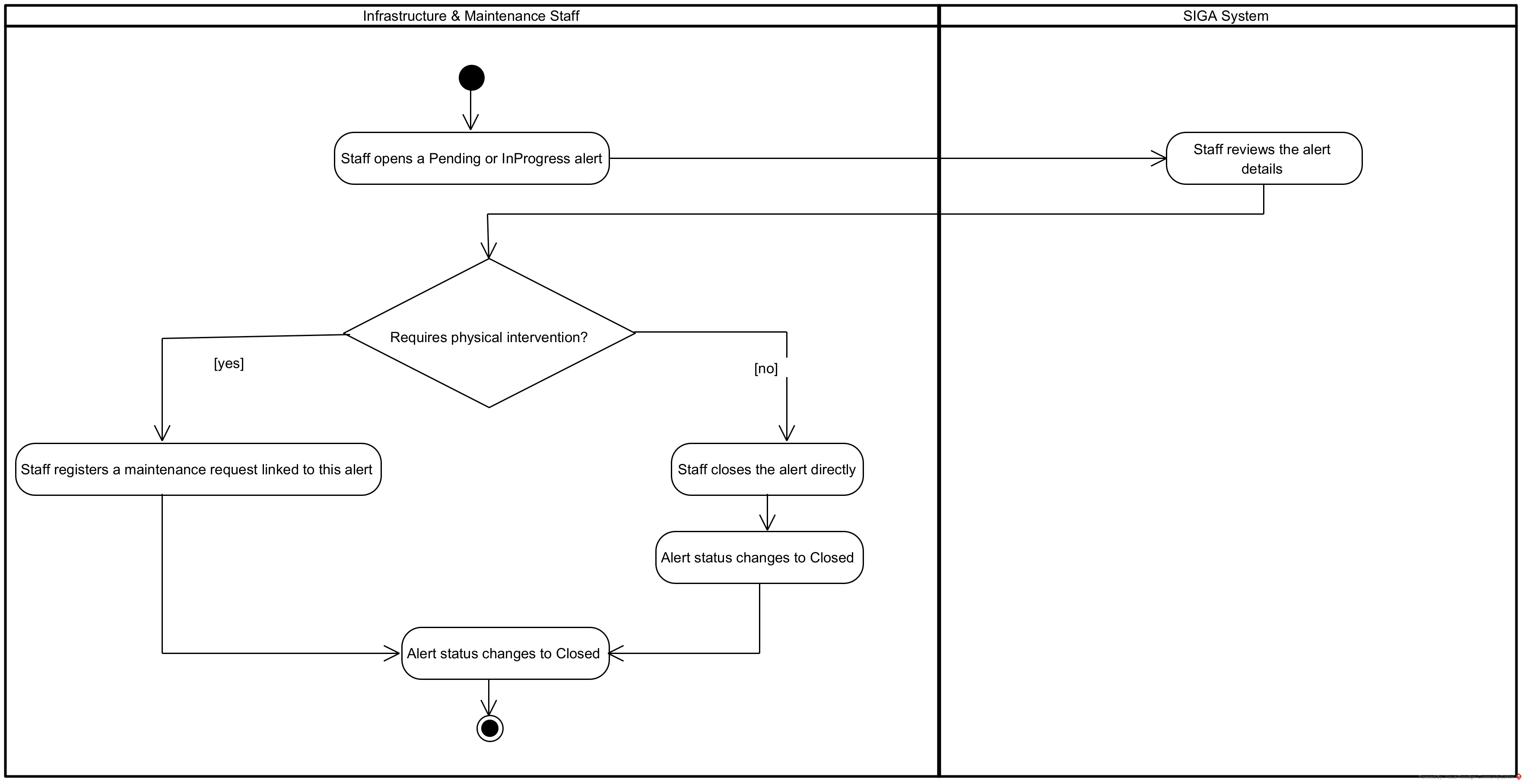
\includegraphics[width=0.85\textwidth,height=0.8\textheight,keepaspectratio]{figuras/act_UC05_attend_anomaly_alert.png}
\caption{Diagrama de actividad --- CU-05 Atender alerta de anomalía}
\label{fig:act-cu05}
\end{figure}

\begin{figure}[H]
\centering
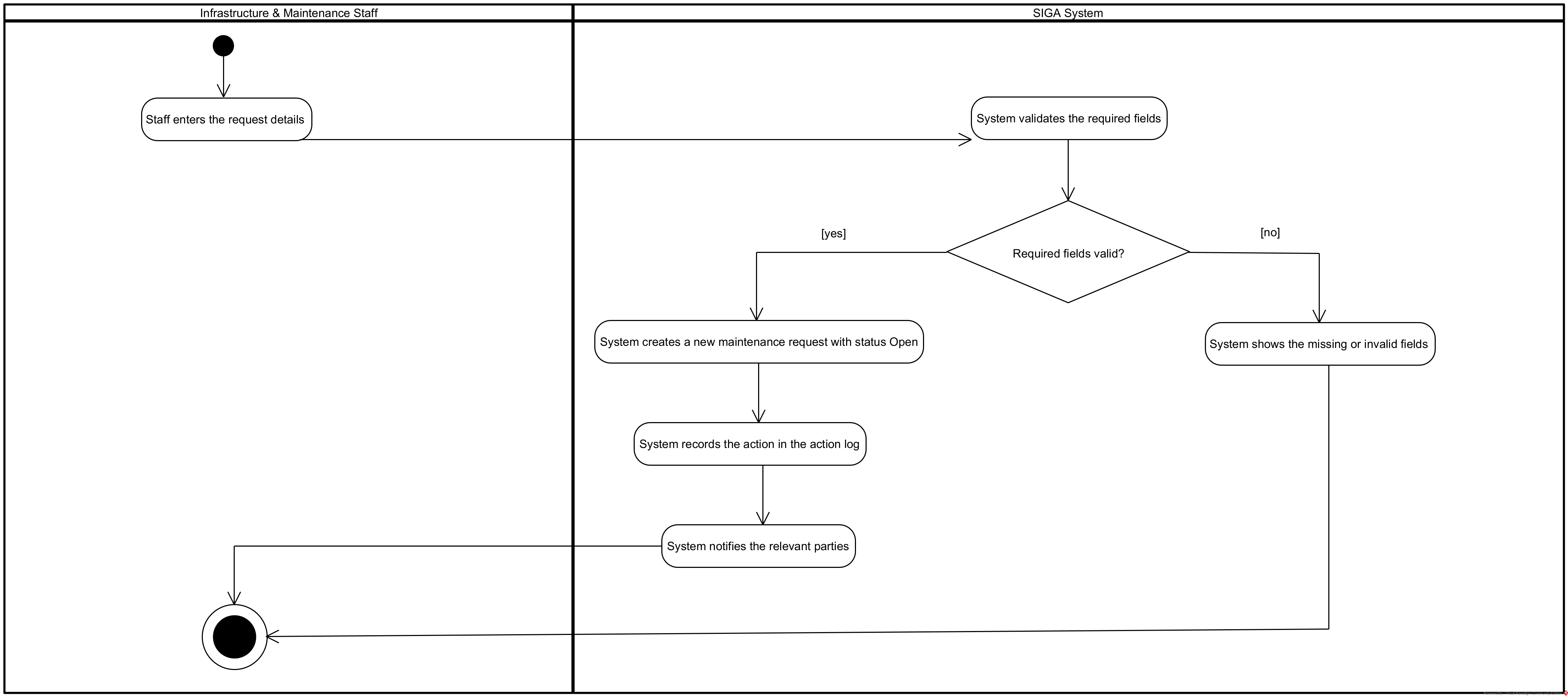
\includegraphics[width=0.85\textwidth,height=0.8\textheight,keepaspectratio]{figuras/act_UC06_register_maintenance_request.png}
\caption{Diagrama de actividad --- CU-06 Registrar solicitud de mantenimiento}
\label{fig:act-cu06}
\end{figure}

\begin{figure}[H]
\centering
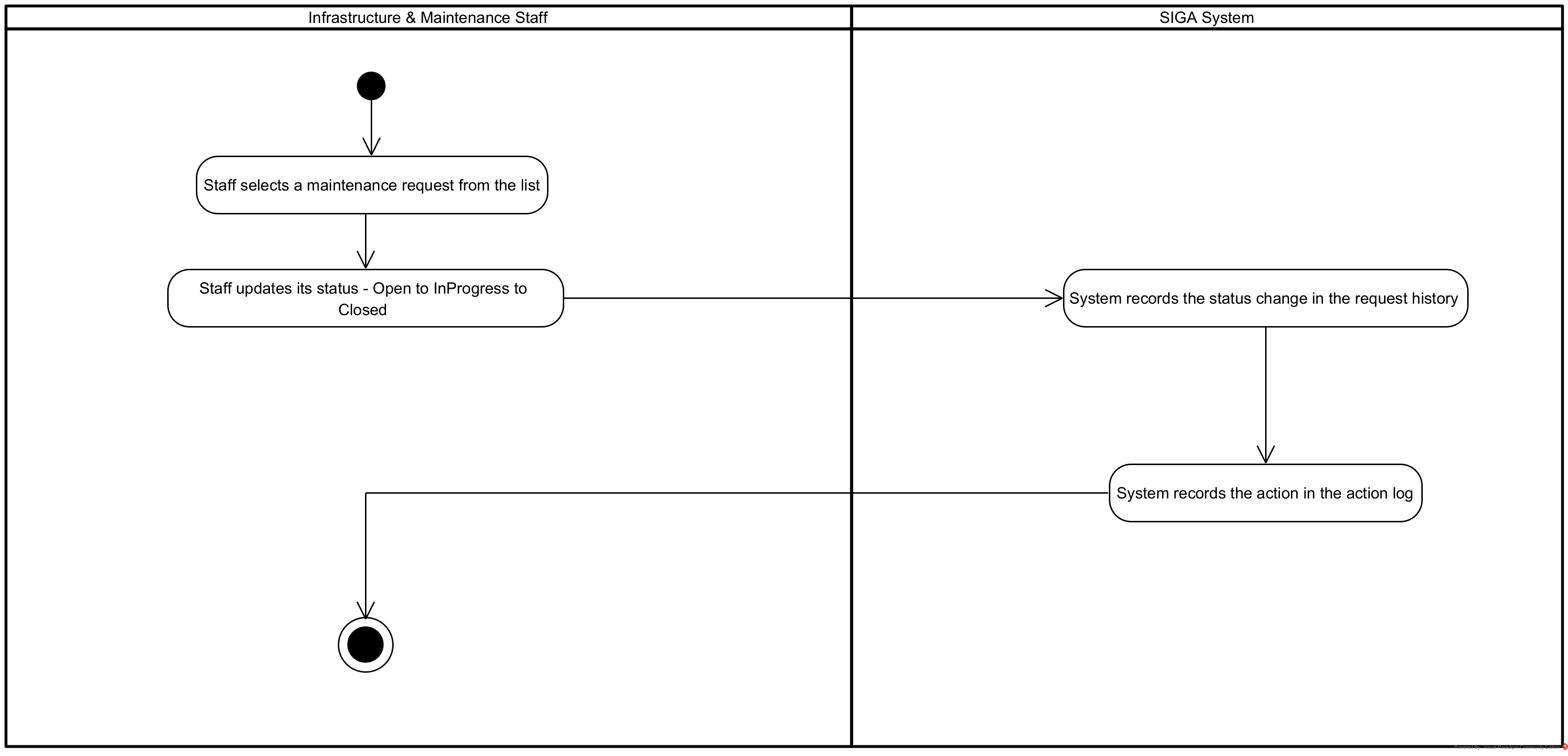
\includegraphics[width=0.85\textwidth,height=0.8\textheight,keepaspectratio]{figuras/act_UC07_track_maintenance_ticket.png}
\caption{Diagrama de actividad --- CU-07 Dar seguimiento a ticket de mantenimiento}
\label{fig:act-cu07}
\end{figure}

\begin{figure}[H]
\centering
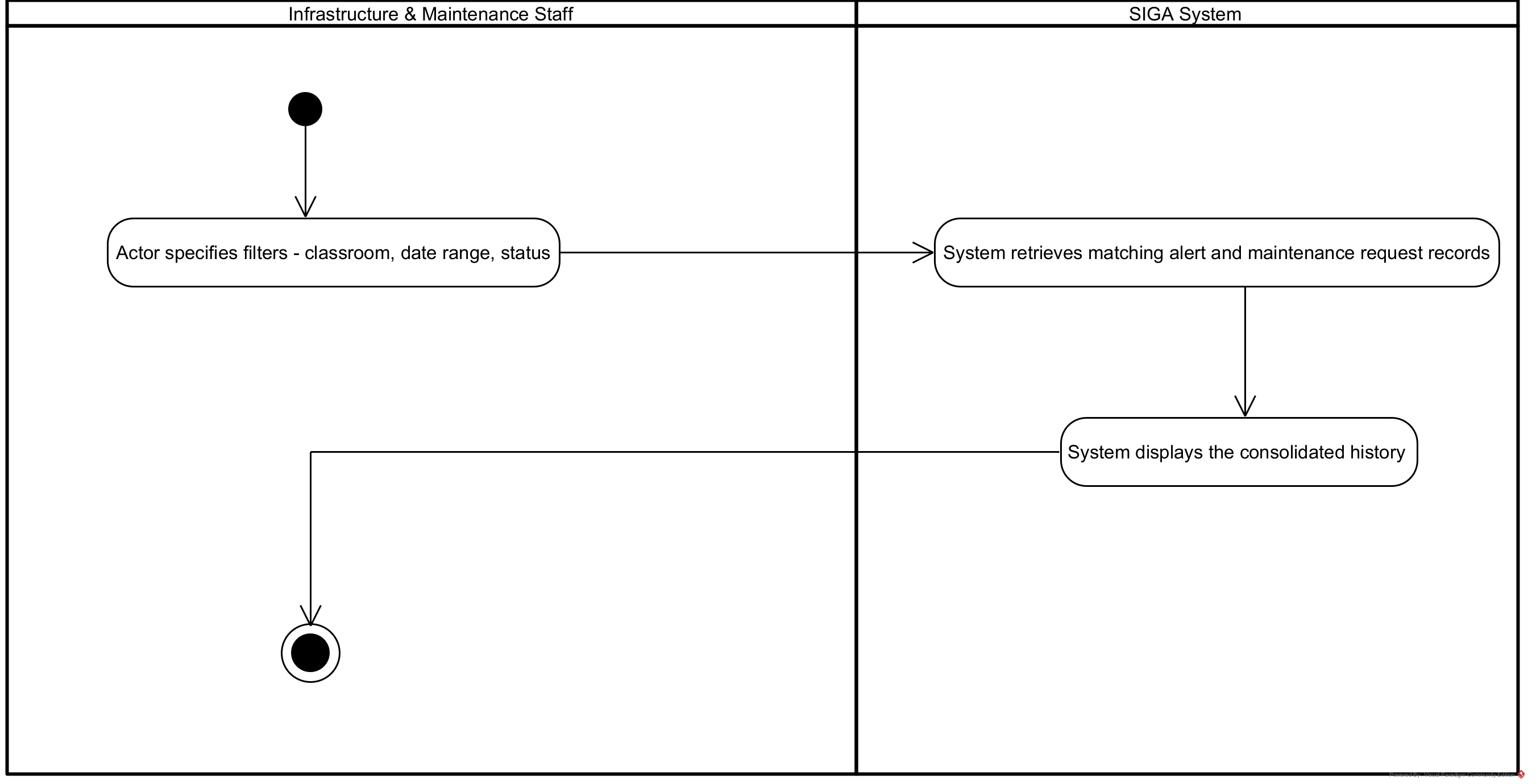
\includegraphics[width=0.85\textwidth,height=0.8\textheight,keepaspectratio]{figuras/act_UC08_view_failure_maintenance_history.png}
\caption{Diagrama de actividad --- CU-08 Consultar historial de fallas y mantenimientos}
\label{fig:act-cu08}
\end{figure}

\begin{figure}[H]
\centering
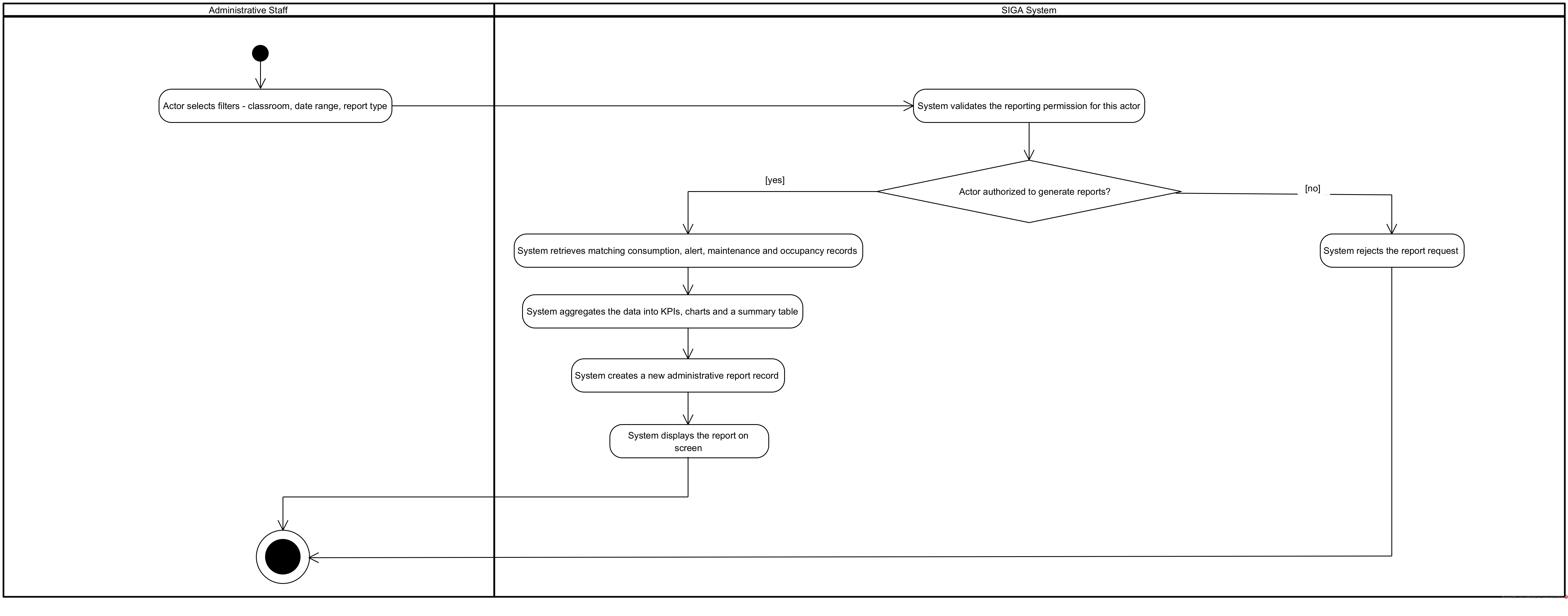
\includegraphics[width=0.85\textwidth,height=0.8\textheight,keepaspectratio]{figuras/act_UC09_generate_administrative_reports.png}
\caption{Diagrama de actividad --- CU-09 Generar reportes administrativos}
\label{fig:act-cu09}
\end{figure}

\begin{figure}[H]
\centering
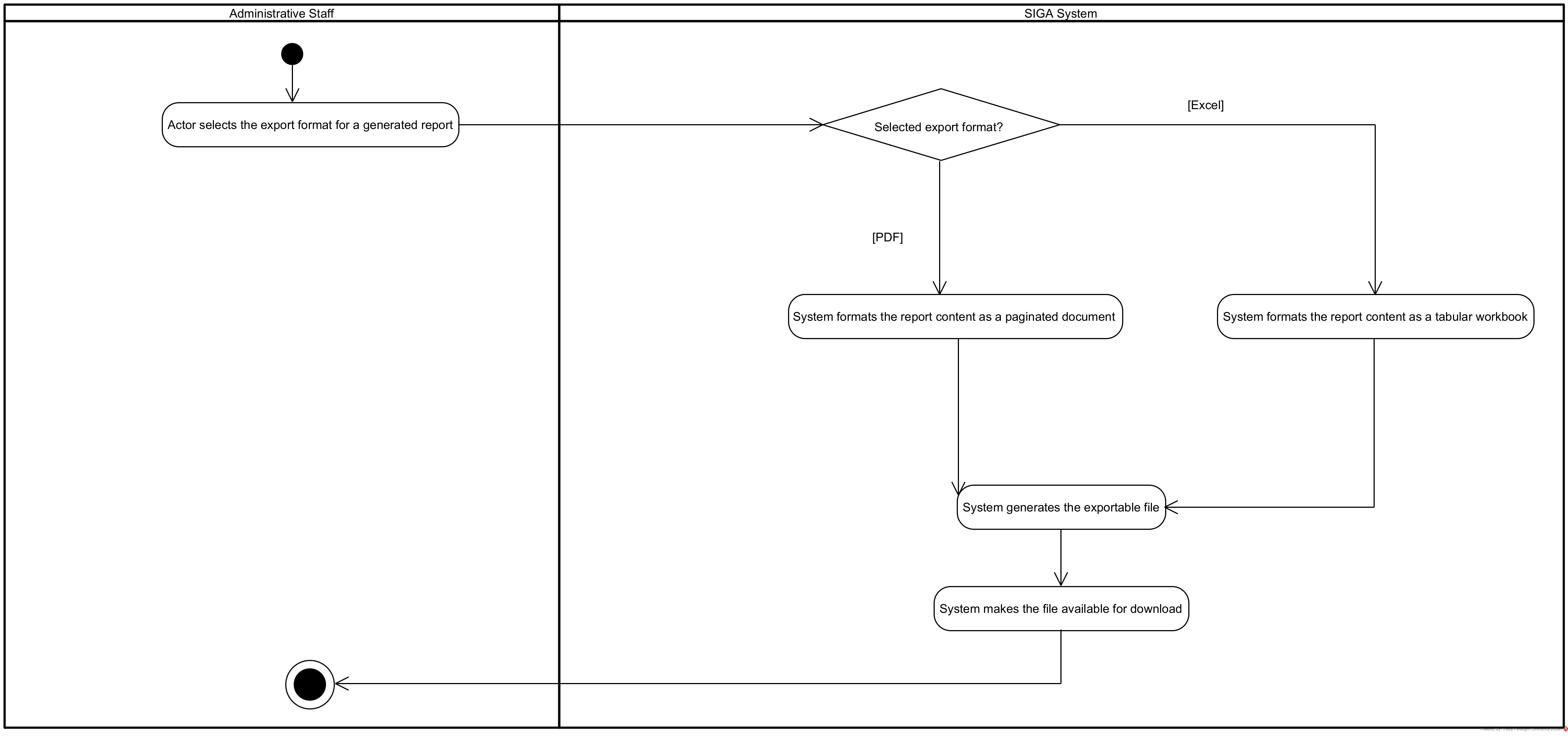
\includegraphics[width=0.85\textwidth,height=0.8\textheight,keepaspectratio]{figuras/act_UC10_export_reports.png}
\caption{Diagrama de actividad --- CU-10 Exportar reportes PDF y Excel}
\label{fig:act-cu10}
\end{figure}

\begin{figure}[H]
\centering
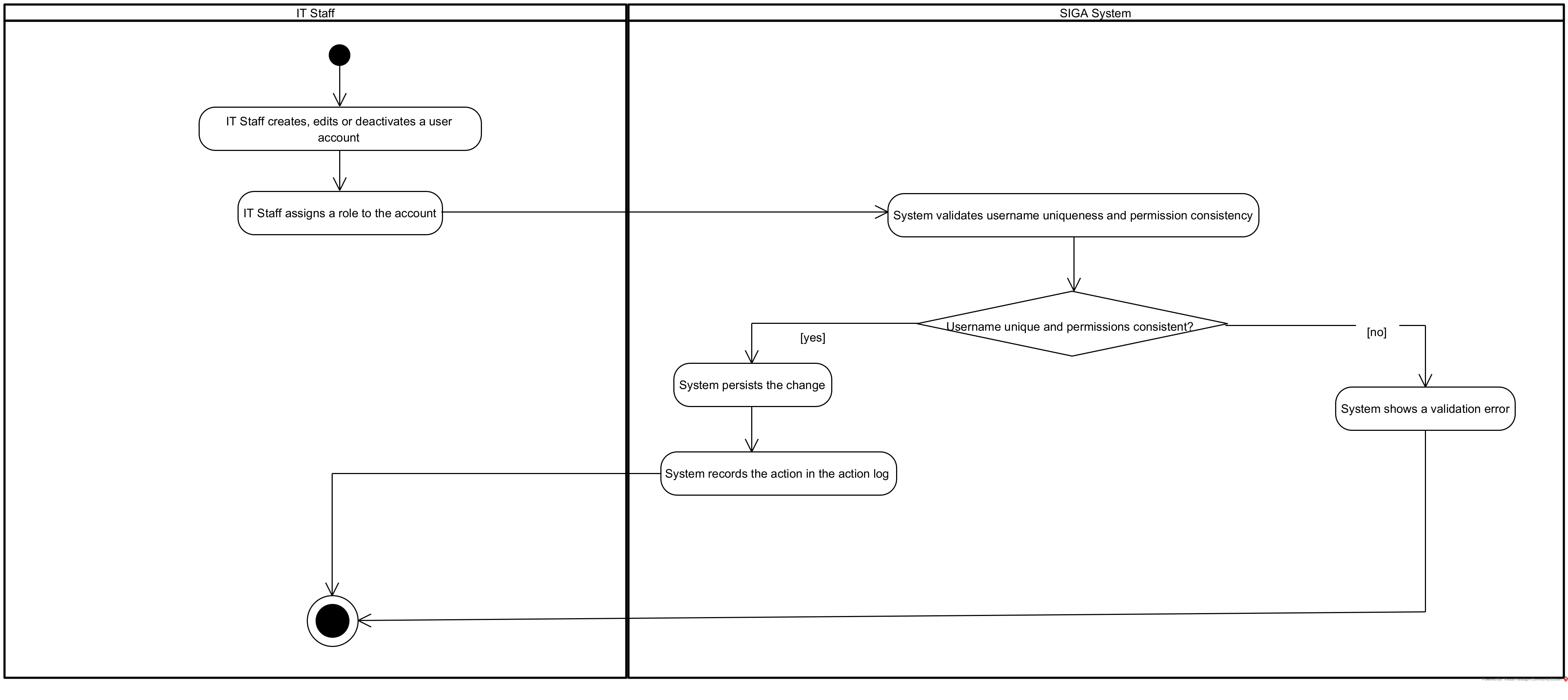
\includegraphics[width=0.85\textwidth,height=0.8\textheight,keepaspectratio]{figuras/act_UC11_manage_users_roles_permissions.png}
\caption{Diagrama de actividad --- CU-11 Gestionar usuarios, roles y permisos}
\label{fig:act-cu11}
\end{figure}

\begin{figure}[H]
\centering
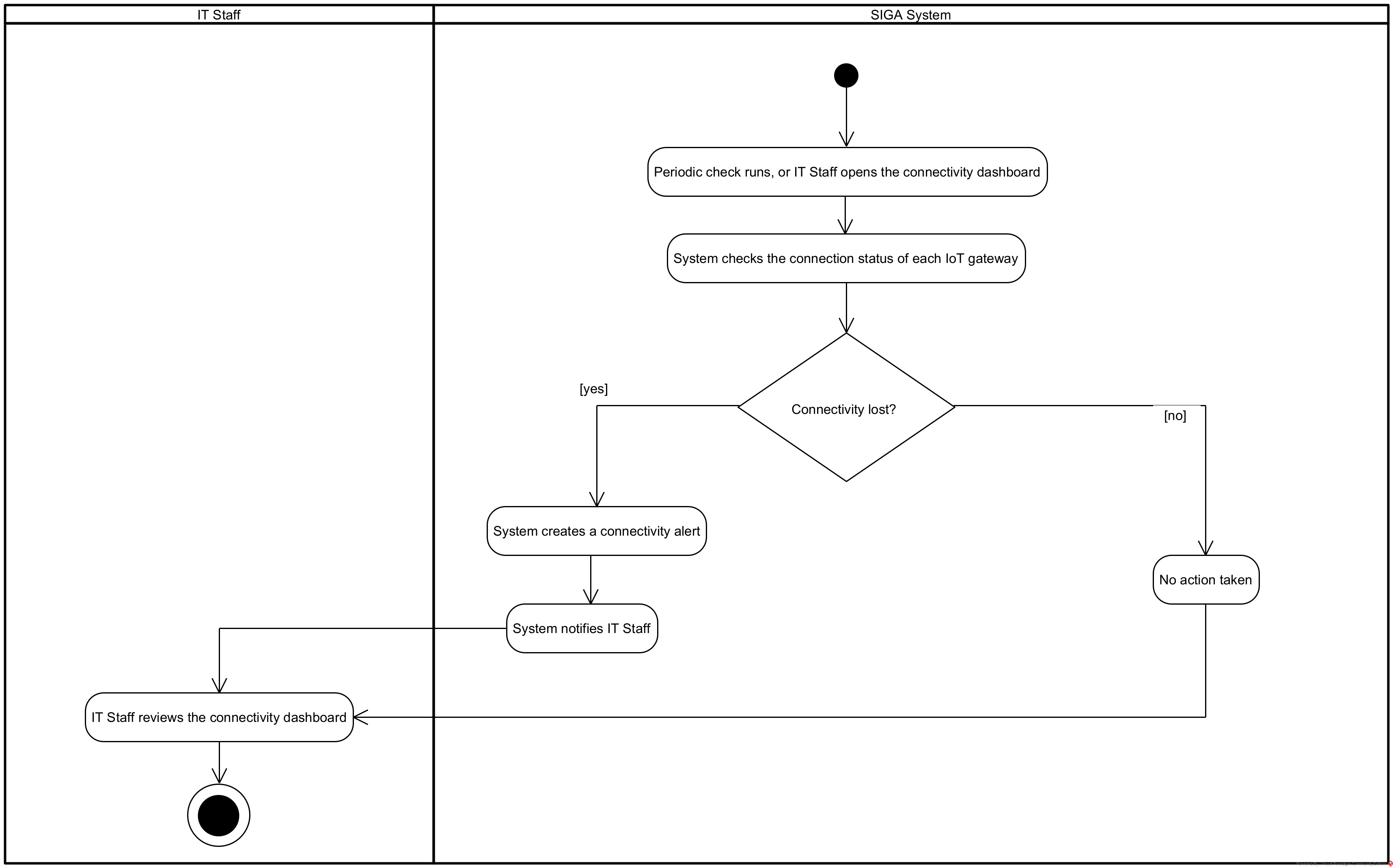
\includegraphics[width=0.85\textwidth,height=0.8\textheight,keepaspectratio]{figuras/act_UC12_monitor_iot_connectivity.png}
\caption{Diagrama de actividad --- CU-12 Monitorear conectividad IoT}
\label{fig:act-cu12}
\end{figure}

\begin{figure}[H]
\centering
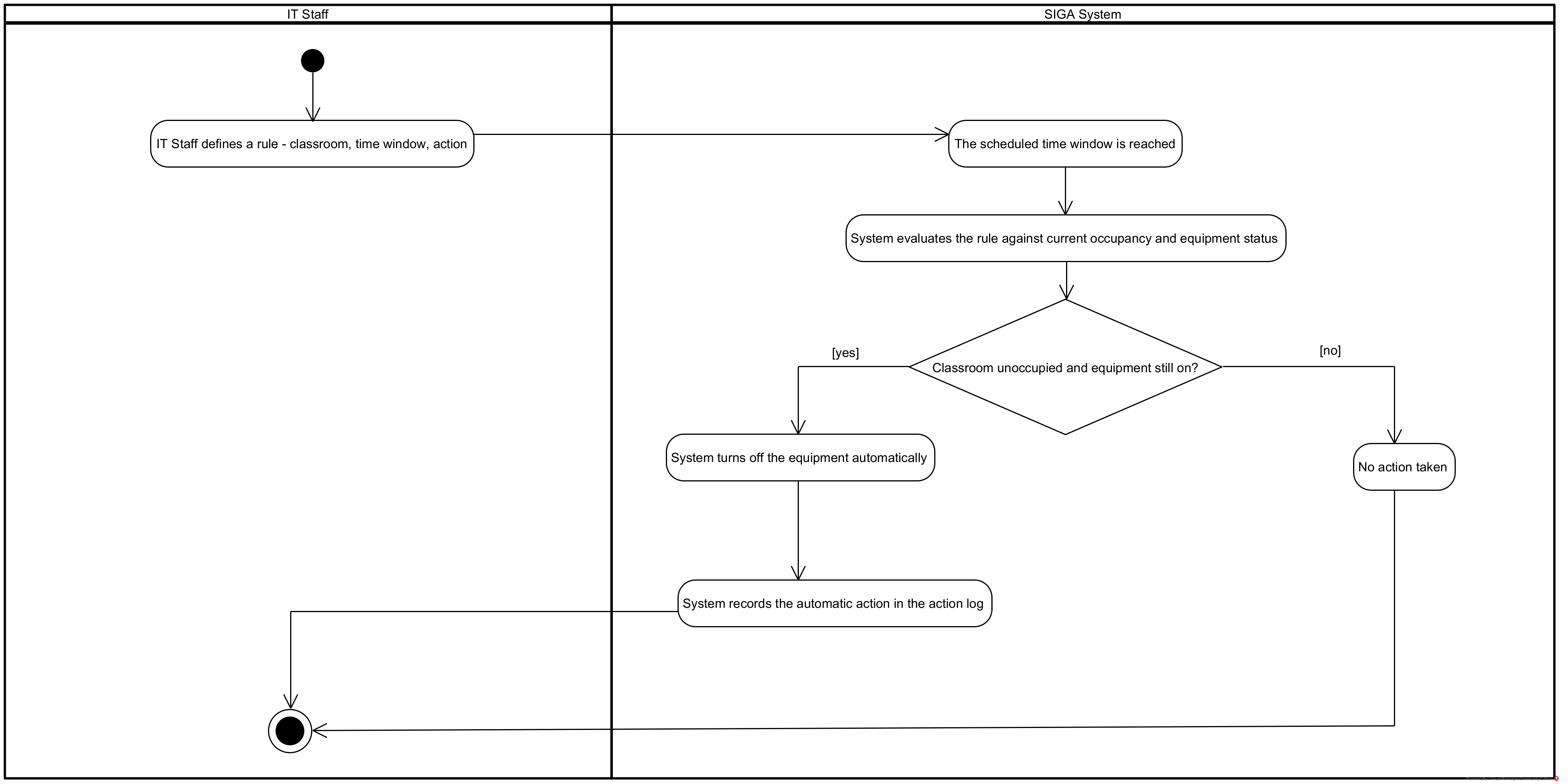
\includegraphics[width=0.85\textwidth,height=0.8\textheight,keepaspectratio]{figuras/act_UC13_schedule_automatic_onoff_rules.png}
\caption{Diagrama de actividad --- CU-13 Programar reglas de encendido y apagado}
\label{fig:act-cu13}
\end{figure}

\begin{figure}[H]
\centering
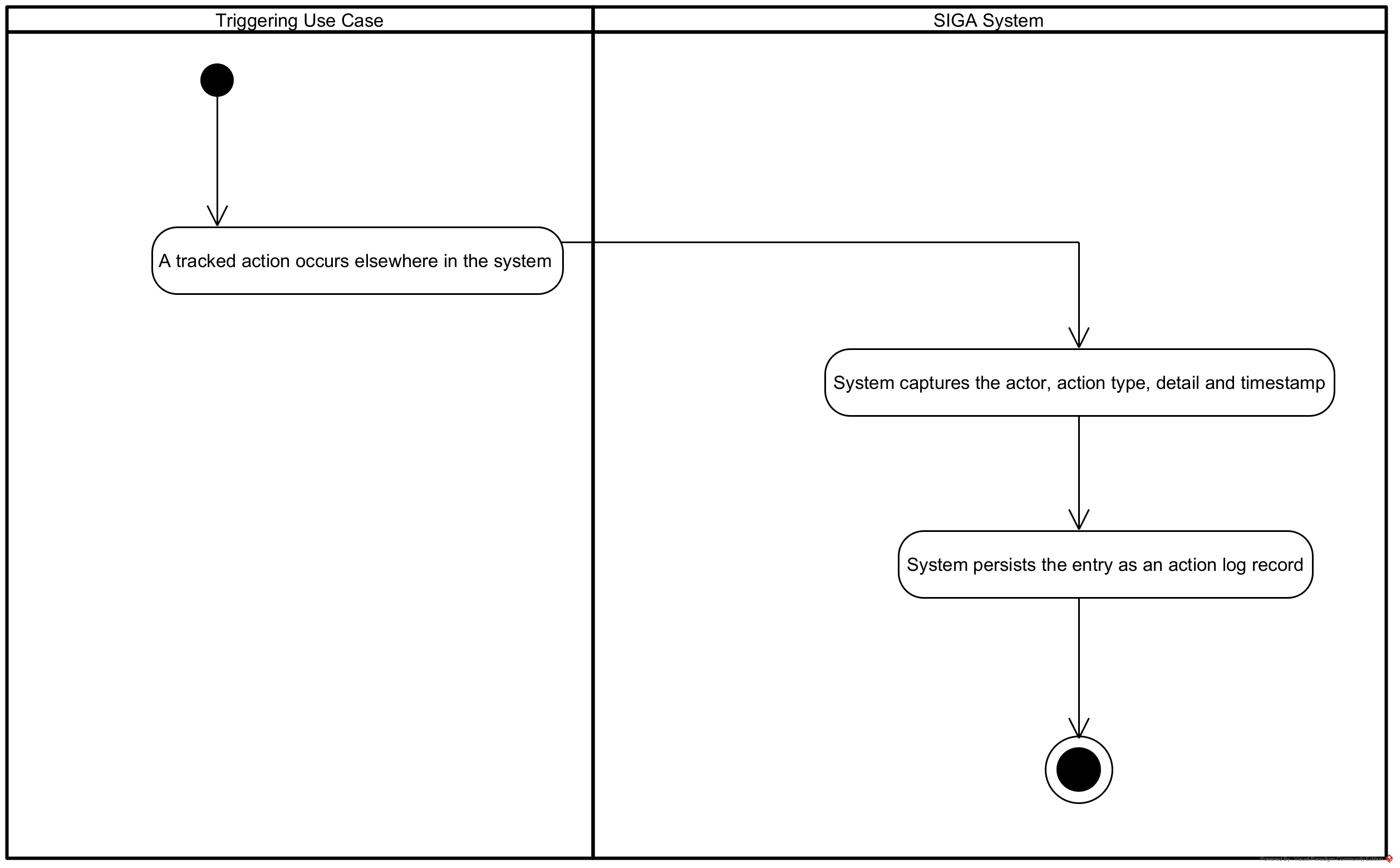
\includegraphics[width=0.85\textwidth,height=0.8\textheight,keepaspectratio]{figuras/act_UC14_log_user_actions.png}
\caption{Diagrama de actividad --- CU-14 Registrar bitácora de acciones}
\label{fig:act-cu14}
\end{figure}

\begin{figure}[H]
\centering
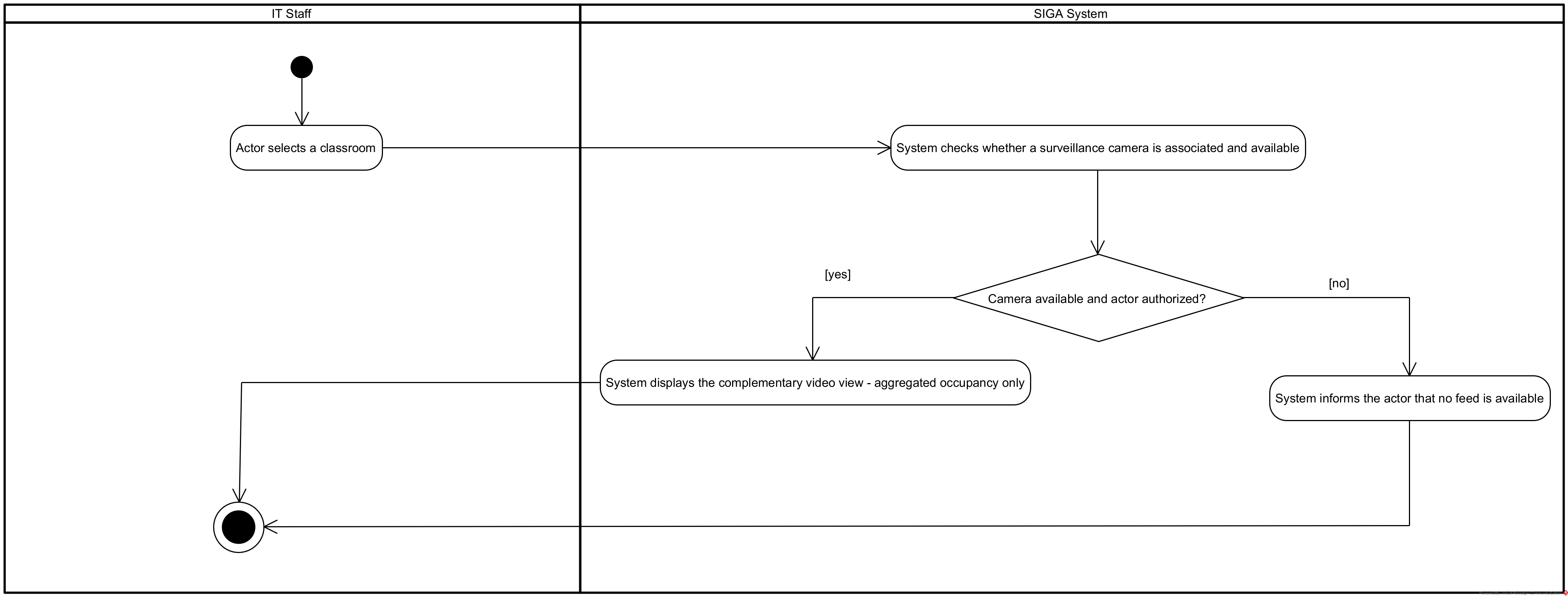
\includegraphics[width=0.85\textwidth,height=0.8\textheight,keepaspectratio]{figuras/act_UC15_view_room_cameras.png}
\caption{Diagrama de actividad --- CU-15 Consultar cámaras asociadas al aula}
\label{fig:act-cu15}
\end{figure}

\begin{figure}[H]
\centering
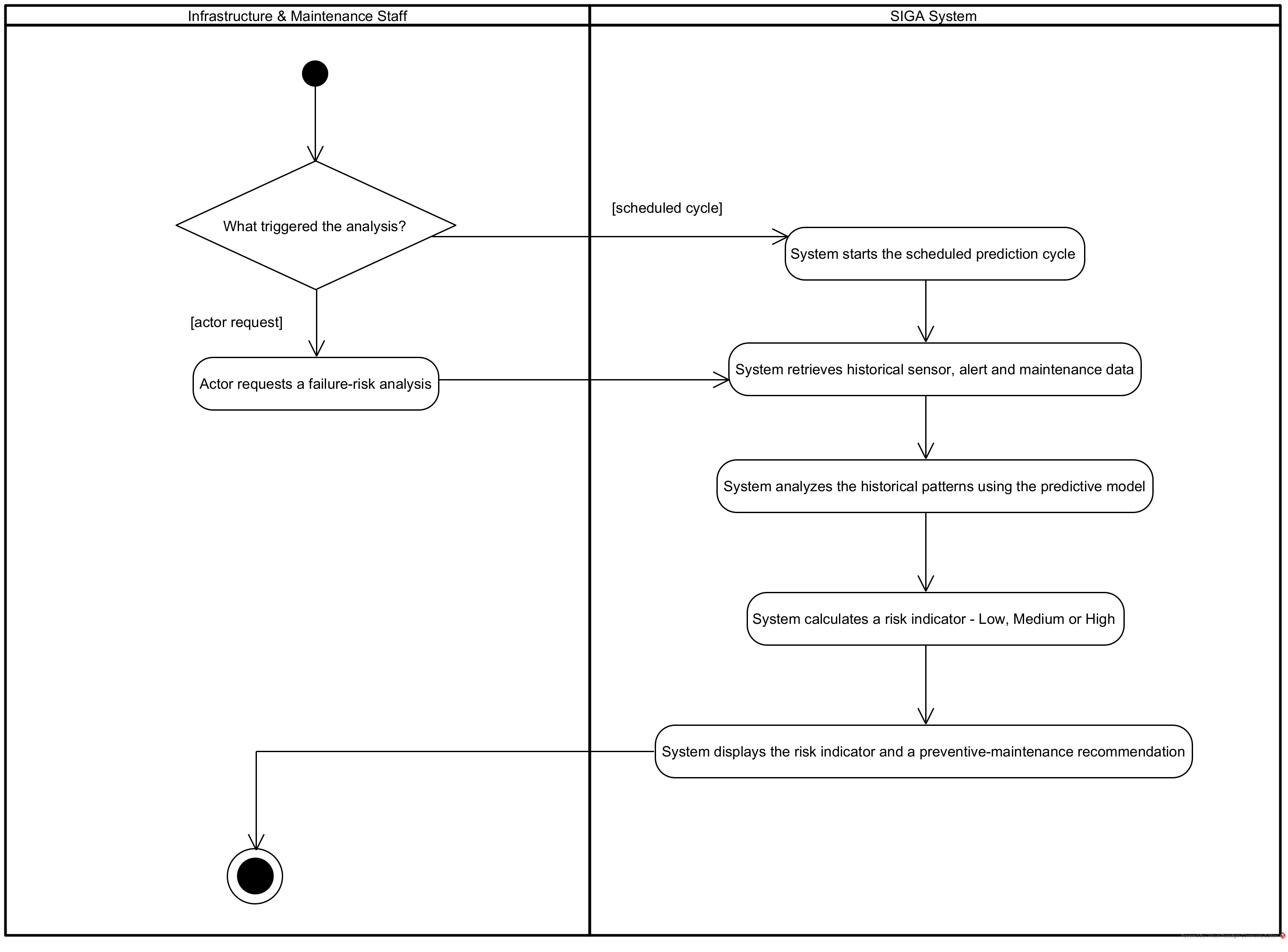
\includegraphics[width=0.85\textwidth,height=0.8\textheight,keepaspectratio]{figuras/act_UC16_predict_equipment_failures.png}
\caption{Diagrama de actividad --- CU-16 Predecir fallas de equipos}
\label{fig:act-cu16}
\end{figure}

\subsection*{4.10 Diagrama de estados --- Alerta}

\addcontentsline{toc}{subsection}{4.10 Diagrama de estados --- Alerta}

\textit{Entidad seleccionada: \textit{Alerta}, segundo ciclo de vida no trivial del dominio. Estados: Generada $\rightarrow$ Notificada $\rightarrow$ \{Atendida | Escalada\}. Transiciones: Generada $\rightarrow$ Notificada (envío automático al responsable); Notificada $\rightarrow$ Atendida (registro de acción del responsable); Notificada $\rightarrow$ Escalada (sin atención dentro del umbral de tiempo definido en RNF-01); Escalada $\rightarrow$ Atendida (intervención de autoridad).}

\begin{figure}[H]
\centering
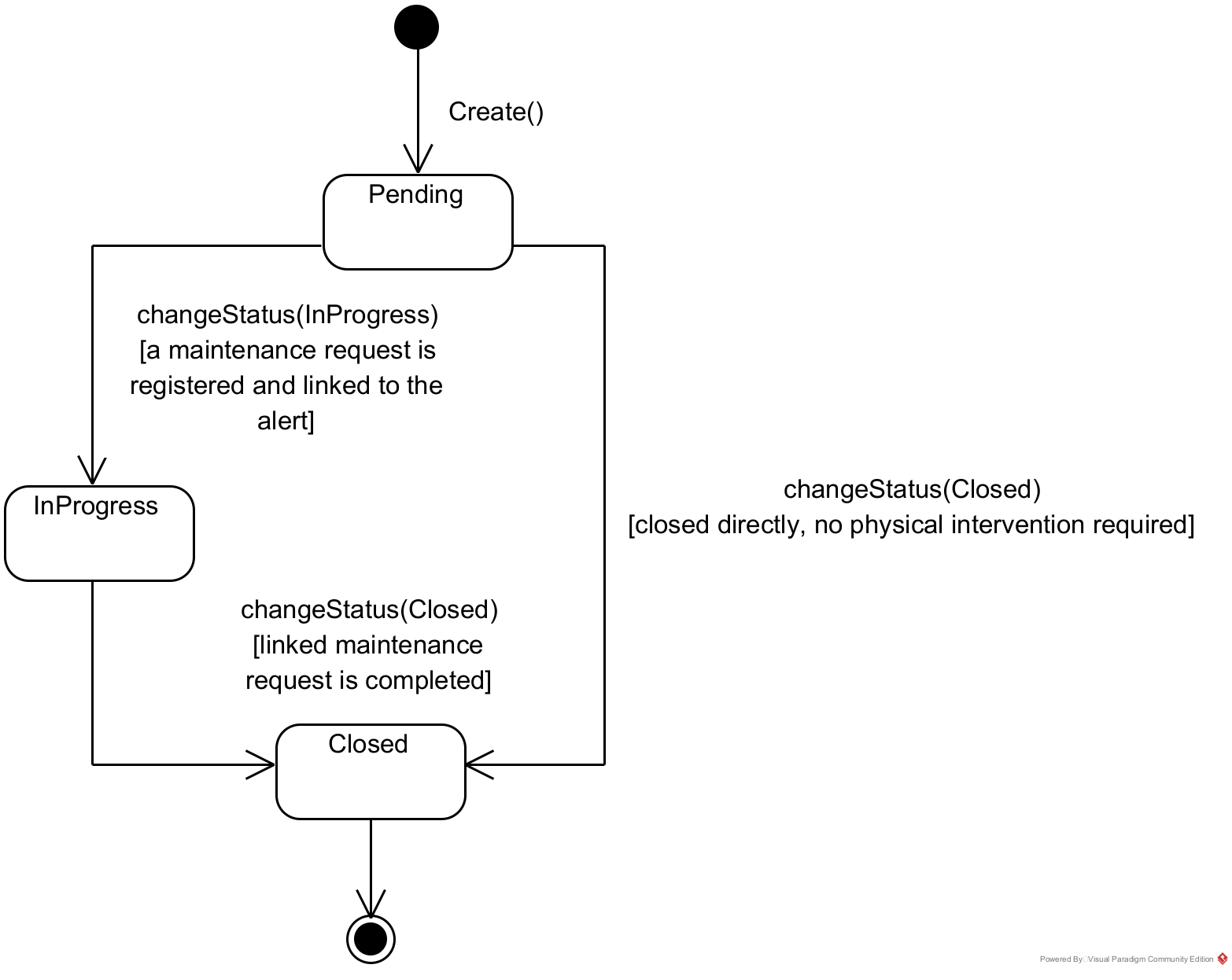
\includegraphics[width=0.85\textwidth,height=0.8\textheight,keepaspectratio]{figuras/state_alert.png}
\caption{Diagrama de estados --- Alerta}
\label{fig:state-alerta}
\end{figure}

\section*{V. PRIORIZACIÓN Y TRAZABILIDAD EXTENDIDA}

\addcontentsline{toc}{section}{V. PRIORIZACIÓN Y TRAZABILIDAD EXTENDIDA}

\subsection*{5.1 Clasificación de requisitos (RF / RNF / restricción)}

\addcontentsline{toc}{subsection}{5.1 Clasificación de requisitos (RF / RNF / restricción)}

La clasificación completa de RF, RNF y restricciones de diseño, con su prioridad MoSCoW, evidencia de origen y justificación, se presenta consolidada en la Tabla 42.


\begingroup
\small
\begin{longtable}{|p{2.6cm}|p{2.6cm}|p{2.6cm}|p{2.6cm}|p{2.6cm}|p{2.6cm}|}
\hline
ID & Nombre & Tipo & Prioridad & Evidencia & Justificación \\ \hline
RF-01 & Recopilación datos ambientales & RF & Must & EV-01 & Sin datos en tiempo real el sistema no puede monitorear, alertar ni automatizar ninguna función. \\ \hline
RF-02 & Control remoto de dispositivos & RF & Must & EV-01 & Elimina el desplazamiento físico para apagar/encender equipos, problema central identificado en EV-01. \\ \hline
RF-03 & Detección automática de ocupación & RF & Must & EV-01 & Requisito base para las reglas de apagado automático (RF-13, RF-16). \\ \hline
RF-04 & Monitoreo y control de proyectores & RF & Must & EV-01, EV-02 & Falla más frecuente según ambas entrevistas. Causa directa de interrupciones de clase. \\ \hline
RF-05 & Monitoreo y ajuste de climatización & RF & Must & EV-01 & Segunda causa de problemas en aulas (EV-01). Impacta directamente en el confort. \\ \hline
RF-06 & Integración con videovigilancia & RF & Should & EV-01 & Complementa el monitoreo visual, pero depende de permisos institucionales. \\ \hline
RF-07 & Panel de control centralizado & RF & Must & EV-01, EV-02 & Es la interfaz principal. Sin el panel, ninguna función es accesible. \\ \hline
RF-08 & Generación y envío de alertas & RF & Must & EV-01 & Mecanismo central de detección y respuesta. \\ \hline
RF-09 & Análisis predictivo de fallos (IA) & RF & Should & EV-02 & Requiere $\geq$30 días de histórico; valioso pero no esencial en fase inicial. \\ \hline
RF-10 & Registro histórico de fallas & RF & Must & EV-01 & Sustituye los informes manuales al decano (EV-01). \\ \hline
RF-11 & Notificación inmediata ante fallas críticas & RF & Must & EV-02 & Las fallas durante clase no se atienden a tiempo; este RF reduce ese tiempo. \\ \hline
RF-12 & Gestión de solicitudes de mantenimiento & RF & Must & EV-01, EV-02 & No existe sistema formal de reporte; es la solución directa al proceso actual. \\ \hline
RF-13 & Control automático de apagado energético & RF & Must & EV-01 & Una sola persona apaga manualmente los equipos; automatizarlo es crítico. \\ \hline
RF-14 & Análisis de patrones de consumo & RF & Should & EV-02 & Agrega valor estratégico pero requiere historial acumulado. \\ \hline
RF-15 & Programación de horarios automatizados & RF & Must & EV-01 & Reduce desperdicio energético al sincronizar con horario académico. \\ \hline
RF-16 & Apagado automático por desocupación & RF & Must & EV-01 & Complemento directo de RF-03 y RF-15. \\ \hline
RF-17 & Reportes estadísticos periódicos & RF & Should & EV-02 & Importante pero no bloquea la operación. \\ \hline
RF-18 & Exportación de reportes PDF/Excel & RF & Should & EV-02 & Agrega valor a RF-17. \\ \hline
RF-19 & Gestión de acceso por roles & RF & Must & EV-02 & Sin control de acceso el sistema no puede desplegarse. \\ \hline
RF-20 & Historial de ocupación de aulas & RF & Should & EV-02 & Depende de acumulación de datos de RF-03. \\ \hline
RF-21 & Notificación equipos fuera de horario & RF & Must & EV-01 & Evita desperdicio energético por equipos sin detección. \\ \hline
RF-22 & Monitoreo de conectividad IoT & RF & Must & EV-01 & Sin monitoreo de conectividad no se garantiza confiabilidad del sistema. \\ \hline
RF-23 & Bitácora de acciones de usuario & RF & Must & EV-01, EV-02 & Necesaria para auditoría interna y cumplimiento de políticas. \\ \hline
RF-24 & Exportación de datos personales & RF & Should & Análisis normativo LOPDP & Soporta el derecho de acceso (Art. 13). \\ \hline
RF-25 & Rectificación de datos personales & RF & Should & Análisis normativo LOPDP & Soporta el derecho de rectificación (Art. 14). \\ \hline
NFR-01 & Alertas en $\leq$60 s & NFR & Must & --- & Tiempo de respuesta crítico para alertas útiles durante una clase en curso. \\ \hline
NFR-02 & Disponibilidad $\geq$99 \% mensual & NFR & Must & --- & El sistema debe operar continuamente. \\ \hline
NFR-03 & Cifrado AES-256 y autenticación & NFR & Must & --- & Requisito de seguridad fundamental para el despliegue institucional. \\ \hline
NFR-10 & Explicabilidad de RF-09 & NFR & Must & --- & Gatekeeper G7: obligatorio para todo componente de IA/ML del sistema. \\ \hline
\caption{Clasificación y priorización de requisitos}
\end{longtable}
\endgroup

\subsection*{5.2 Priorización MoSCoW justificada}

\addcontentsline{toc}{subsection}{5.2 Priorización MoSCoW justificada}

\subsubsection*{5.2.1. Must (críticos - el sistema no funciona sin ellos)}

\addcontentsline{toc}{subsubsection}{5.2.1. Must (críticos - el sistema no funciona sin ellos)}

RF-01 a RF-05, RF-07, RF-08, RF-10 a RF-13, RF-15, RF-16, RF-19, RF-21 a RF-23 constituyen la funcionalidad central del sistema, según el detalle de justificación de la Tabla 42.


\subsubsection*{5.2.2. Should (importantes - agregan valor significativo pero el sistema opera sin ellos)}

\addcontentsline{toc}{subsubsection}{5.2.2. Should (importantes - agregan valor significativo pero el sistema opera sin ellos)}

RF-06, RF-09, RF-14, RF-17, RF-18, RF-20, RF-24 y RF-25 enriquecen la propuesta de valor sin bloquear la operación básica.


\subsubsection*{5.2.3. Could (deseables - se incluirán si el tiempo y los recursos lo permiten)}

\addcontentsline{toc}{subsubsection}{5.2.3. Could (deseables - se incluirán si el tiempo y los recursos lo permiten)}

Candidatos para entregas posteriores: control de iluminación, aplicación móvil nativa y alertas por SMS.


\subsubsection*{5.2.4. Won't (fuera del alcance de esta entrega)}

\addcontentsline{toc}{subsubsection}{5.2.4. Won't (fuera del alcance de esta entrega)}

Integración con el sistema de matrícula y asistencia, control de la red eléctrica general del campus, mantenimiento físico de equipos, y administración de equipos sin compatibilidad IoT (RD-16, RD-17, RD-18).


\subsection*{5.3 Modelo de Kano}

\addcontentsline{toc}{subsection}{5.3 Modelo de Kano}

Nuevo en esta entrega. El cuestionario de estudiantes v2.0 (EV-17, $n=27$--$30$ según pregunta) incluyó únicamente 3 pares genuinos de preguntas funcional/disfuncional (P23-24, P25-26, P27-28), aplicados a RF-05, RF-07 y RF-08. RF-09 y RF-12 no contaron con instrumento Kano en el cuestionario efectivamente aplicado, por lo que se reportan como no clasificados en esta entrega --- no se fabrica una clasificación sin el sustento estadístico correspondiente (regla anti-fabricación de la guía, gatekeeper G4). Los resultados obtenidos, usando la tabla de evaluación Kano estándar, son los siguientes:


\begingroup
\small
\begin{longtable}{|p{3.9cm}|p{3.9cm}|p{3.9cm}|p{3.9cm}|}
\hline
ID-RF & Nombre & Clasificación Kano & Fuente de datos \\ \hline
RF-05 & Ajuste remoto de climatización & Indiferente (37\%, categoría dominante clara) & Cuestionario estudiantes P23/P24 (EV-17, $n=27$--$30$) \\ \hline
RF-08 & Generación y envío de alertas & Sin categoría dominante --- empate a tres bandas (Must-be = One-dimensional = Indiferente, 8 respuestas c/u) & Cuestionario estudiantes P25/P26 (EV-17) \\ \hline
RF-07 & Panel de control centralizado & Sin categoría dominante --- empate a dos bandas (One-dimensional = Attractive, 9 respuestas c/u) & Cuestionario estudiantes P27/P28 (EV-17) \\ \hline
RF-09 & Análisis predictivo de fallos (IA) & Sin clasificar --- no se incluyó par funcional/disfuncional en el instrumento aplicado & N/A \\ \hline
RF-12 & Gestión de solicitudes de mantenimiento & Sin clasificar --- no se incluyó par funcional/disfuncional en el instrumento aplicado & N/A \\ \hline
\caption{Clasificación Kano --- resultados reales del cuestionario EV-17}
\end{longtable}
\endgroup

Se declara como limitación honesta que, salvo RF-05, los resultados Kano no arrojan una categoría dominante clara con el tamaño de muestra actual (RF-07 y RF-08 presentan empates entre bandas). Esto no invalida el instrumento, pero indica que la clasificación de RF-07 y RF-08 debe tratarse como preliminar y ampliarse con mayor muestra en la Entrega 4 (2B) antes de usarla como criterio único de priorización.

\subsection*{5.4 Valor de negocio - WSJF (Weighted Shortest Job First)}

\addcontentsline{toc}{subsection}{5.4 Valor de negocio - WSJF (Weighted Shortest Job First)}

Nuevo en esta entrega. El puntaje WSJF se calcula como (Valor de negocio + Criticidad de tiempo + Reducción de riesgo) / Duración estimada. Los componentes del costo de retraso deben estimarse en sesión de equipo con al menos un stakeholder validando la escala relativa (Fibonacci 1-2-3-5-8-13); se deja la estructura lista para completar durante la semana 13 del cronograma.


\begingroup
\small
\begin{longtable}{|p{2.6cm}|p{2.6cm}|p{2.6cm}|p{2.6cm}|p{2.6cm}|p{2.6cm}|}
\hline
ID-RF & Valor de negocio (1-13) & Criticidad de tiempo (1-13) & Reducción de riesgo (1-13) & Duración estimada (1-13) & WSJF \\ \hline
RF-11 --- Notificación inmediata ante fallas críticas & 8 & 13 & 3 & 3 & 8.0 \\ \hline
RF-08 --- Generación y envío de alertas por anomalías & 13 & 13 & 5 & 5 & 6.2 \\ \hline
RF-19 --- Gestión de acceso diferenciado por roles & 8 & 8 & 13 & 5 & 5.8 \\ \hline
RF-03 --- Detección automática de ocupación de aula & 8 & 5 & 13 & 5 & 5.2 \\ \hline
RF-22 --- Monitoreo de conectividad de red IoT & 5 & 5 & 5 & 3 & 5.0 \\ \hline
RF-04 --- Monitoreo y control remoto de proyectores & 13 & 8 & 3 & 5 & 4.8 \\ \hline
RF-23 --- Registro de bitácora de acciones de usuario & 5 & 3 & 5 & 3 & 4.33 \\ \hline
RF-21 --- Notificación de equipos encendidos fuera de horario & 5 & 5 & 2 & 3 & 4.0 \\ \hline
RF-10 --- Registro histórico de fallas y mantenimientos & 5 & 3 & 3 & 3 & 3.67 \\ \hline
RF-07 --- Panel de control centralizado & 13 & 8 & 8 & 8 & 3.625 \\ \hline
RF-16 --- Apagado automático por aula desocupada & 5 & 3 & 2 & 3 & 3.33 \\ \hline
RF-12 --- Gestión de solicitudes de mantenimiento & 13 & 8 & 5 & 8 & 3.25 \\ \hline
RF-01 --- Recopilación de datos ambientales mediante sensores IoT & 5 & 3 & 8 & 5 & 3.2 \\ \hline
RF-05 --- Monitoreo y ajuste remoto de climatización & 8 & 5 & 3 & 5 & 3.2 \\ \hline
RF-13 --- Control automático de apagado energético & 8 & 3 & 2 & 5 & 2.6 \\ \hline
RF-15 --- Programación de horarios automatizados & 5 & 3 & 5 & 5 & 2.6 \\ \hline
RF-02 --- Monitoreo y control remoto de dispositivos & 8 & 5 & 3 & 8 & 2.0 \\ \hline
\caption{Priorización WSJF}
\end{longtable}
\endgroup

\subsection*{5.5 Matriz de trazabilidad extendida}

\addcontentsline{toc}{subsection}{5.5 Matriz de trazabilidad extendida}

La matriz de 1B contenía 28 filas (EV $\rightarrow$ RF $\rightarrow$ CU). Se presenta a continuación con las columnas heredadas; las columnas nuevas exigidas por la guía 2A (Ley $\rightarrow$ Artículo, ID-HU, ID-CA, ID-Componente, ID-Mockup) se agregan en el archivo 04\_Trazabilidad/matriz\_trazabilidad.csv del repositorio, donde también se completan las $\geq$11 filas adicionales necesarias para alcanzar el mínimo de 40 (correspondientes a RF-24, RF-25, los RNF nuevos y las nuevas evidencias de campo EV-08 en adelante).


\begingroup
\small
\begin{longtable}{|p{3.1cm}|p{3.1cm}|p{3.1cm}|p{3.1cm}|p{3.1cm}|}
\hline
ID-EV & Evidencia (fuente) & ID Req. & Nombre del requisito & Caso(s) de uso \\ \hline
EV-01 & Personal de Infraestructura 14/05/2026 & RF-01 & Recopilación datos ambientales (sensores IoT) & CU-01, CU-03 \\ \hline
EV-01 & Personal de Infraestructura 14/05/2026 & RF-02 & Monitoreo y control remoto de dispositivos & CU-02 \\ \hline
EV-01 & Personal de Infraestructura 14/05/2026 & RF-03 & Detección automática de ocupación & CU-03 \\ \hline
EV-01, EV-02, EV-03 & Infraestructura (14/05) + Coordinación (30/06) + Estudiantes (01/07) & RF-04 & Monitoreo y control remoto de proyectores & CU-01, CU-02 \\ \hline
EV-01, EV-03 & Infraestructura (14/05) + Estudiantes (01/07) & RF-05 & Monitoreo y ajuste remoto de climatización & CU-01, CU-02 \\ \hline
EV-01 & Personal de Infraestructura 14/05/2026 & RF-06 & Integración con el sistema de videovigilancia & CU-15 \\ \hline
EV-01, EV-02, EV-03 & Infraestructura (14/05) + Coordinación (30/06) + Estudiantes (01/07) & RF-07 & Panel de control centralizado & CU-01 \\ \hline
EV-01, EV-03 & Infraestructura (14/05) + Estudiantes (01/07) & RF-08 & Generación y envío de alertas por anomalías & CU-04, CU-05 \\ \hline
EV-02 & Coordinación de la Carrera 30/06/2026 & RF-09 & Análisis predictivo de fallos mediante IA & CU-16 \\ \hline
EV-01 & Personal de Infraestructura 14/05/2026 & RF-10 & Registro histórico de fallas y mantenimientos & CU-08 \\ \hline
EV-02, EV-03 & Coordinación (30/06) + Estudiantes (01/07) & RF-11 & Notificación inmediata ante fallas críticas & CU-04, CU-05 \\ \hline
EV-01, EV-02, EV-03 & Infraestructura (14/05) + Coordinación (30/06) + Estudiantes (01/07) & RF-12 & Gestión de solicitudes de mantenimiento & CU-06, CU-07 \\ \hline
EV-01 & Personal de Infraestructura 14/05/2026 & RF-13 & Control automático de apagado energético & CU-13 \\ \hline
EV-02 & Coordinación de la Carrera 30/06/2026 & RF-14 & Análisis de patrones de consumo energético & CU-16 \\ \hline
EV-01 & Personal de Infraestructura 14/05/2026 & RF-15 & Programación de horarios automatizados & CU-13 \\ \hline
EV-01 & Personal de Infraestructura 14/05/2026 & RF-16 & Apagado automático por aula desocupada & CU-03, CU-13 \\ \hline
EV-02 & Coordinación de la Carrera 30/06/2026 & RF-17 & Generación de reportes estadísticos periódicos & CU-09 \\ \hline
EV-02 & Coordinación de la Carrera 30/06/2026 & RF-18 & Exportación de reportes PDF/Excel & CU-10 \\ \hline
EV-02 & Coordinación de la Carrera 30/06/2026 & RF-19 & Gestión de acceso diferenciado por roles & CU-11 \\ \hline
EV-02 & Coordinación de la Carrera 30/06/2026 & RF-20 & Registro del historial de ocupación & CU-01, CU-08 \\ \hline
EV-01 & Personal de Infraestructura 14/05/2026 & RF-21 & Notificación equipos encendidos fuera de horario & CU-04, CU-13 \\ \hline
EV-01 & Personal de Infraestructura 14/05/2026 & RF-22 & Monitoreo de conectividad de red IoT & CU-12 \\ \hline
EV-01, EV-02 & Infraestructura (14/05) + Coordinación (30/06) & RF-23 & Registro de bitácora de acciones de usuario & CU-14 \\ \hline
EV-03 & Estudiantes de la Carrera de Software, 01/07/2026 & RF-04, RF-05, RF-07, RF-08, RF-11, RF-12, RF-22 & Validación complementaria mediante cuestionario digital aplicado a estudiantes & CU-01, CU-02, CU-04, CU-05, CU-06, CU-07, CU-12 \\ \hline
EV-04 & Fotografías de las sesiones EV-01 y EV-02 & RF-01 a RF-05, RF-07, RF-08 & Evidencia fotográfica del trabajo de campo, entrevistas y contexto físico observado & CU-01, CU-02, CU-03, CU-04 \\ \hline
EV-05 & Documento institucional: horario académico vigente & RF-13, RF-15, RF-16, RF-20, RF-21; RD-13 & Horario académico vigente & CU-03, CU-09, CU-13 \\ \hline
EV-06 & Video AS-IS: proceso de mantenimiento físico de equipos en aulas & RF-08, RF-10, RF-11, RF-12, RF-17; RD-17 & Registro o informe de mantenimiento & CU-04, CU-08, CU-09 \\ \hline
EV-07 & Documento institucional: evidencia del sistema de cámaras & RF-06, RF-07, RF-22; RD-05 & Evidencia del sistema de cámaras de videovigilancia & CU-01, CU-12, CU-15 \\ \hline
\caption{Matriz de trazabilidad (base heredada de 1B, 29 filas)}
\end{longtable}
\endgroup

\section*{VI. PRODUCTO MÍNIMO VIABLE (MVP) FUNCIONAL}

\addcontentsline{toc}{section}{VI. PRODUCTO MÍNIMO VIABLE (MVP) FUNCIONAL}

Nuevo en esta entrega. Repositorio Git separado y público con el código fuente del MVP.


\subsection*{6.1 Alcance del MVP}

\addcontentsline{toc}{subsection}{6.1 Alcance del MVP}

Se propone cubrir el 60\% de los RF Must priorizando los de menor complejidad técnica de demostración: RF-01, RF-02, RF-03, RF-04, RF-05, RF-07, RF-08, RF-10, RF-11, RF-12, RF-13, RF-15. Esto representa 12 de 17 RF Must (71\%), superando el mínimo exigido del 60\%.


\subsection*{6.2 Arquitectura propuesta}

\addcontentsline{toc}{subsection}{6.2 Arquitectura propuesta}

Frontend web (panel de control, alertas, mantenimiento), API REST como orquestador, base de datos relacional, simulador de sensores IoT (en ausencia de hardware físico desplegado) que publica lecturas sintéticas vía MQTT hacia un broker local, replicando el comportamiento de un Gateway IoT real para efectos de demostración.


\subsection*{6.3 Instrucciones de despliegue}

\addcontentsline{toc}{subsection}{6.3 Instrucciones de despliegue}

El repositorio del MVP deberá incluir un README.md con instrucciones de despliegue local (docker compose up o equivalente), la cobertura de RF Must marcada explícitamente, y el video de demostración de duración $\leq$3 minutos en 05\_MVP/video\_demo.mp4.


\subsection*{6.4 Estado actual}

\addcontentsline{toc}{subsection}{6.4 Estado actual}

El MVP está implementado en un repositorio separado (https://github.com/gsanchezc6-beep/SIGA\_FGMMN\_MVP), cubriendo 11 de los 17 RF Must (64,7\%), verificado contra el código real: autenticación y roles (RF-19), panel de control (RF-01, RF-03, RF-07, RF-22), alertas (RF-08), apagado automático (RF-13, RF-16), gestión de mantenimiento (RF-10, RF-12) y bitácora (RF-23). Incluye un simulador de sensores que genera lecturas sintéticas y dispara alertas automáticamente durante la demostración. El video de demostración ($\leq$3 minutos) se encuentra en 05\_MVP/video\_demo.mp4 del repositorio del ERS.


\section*{VII. COMPONENTE EMPÍRICO - PROTOCOLO EXPERIMENTAL (RESUMEN)}

\addcontentsline{toc}{section}{VII. COMPONENTE EMPÍRICO - PROTOCOLO EXPERIMENTAL (RESUMEN)}

Nuevo en esta entrega. El protocolo completo debe registrarse en OSF (https://osf.io) ANTES de iniciar cualquier recolección de datos nueva del experimento (gatekeeper G6). Este apartado resume el diseño; el detalle completo reside en 06\_Experimento/protocolo.pdf.


\subsection*{7.1 Enfoque elegido y preguntas de investigación (PICOC)}

\addcontentsline{toc}{subsection}{7.1 Enfoque elegido y preguntas de investigación (PICOC)}

Enfoque 1: comparación de la calidad de los Requisitos Funcionales elicitados por el equipo humano frente a los generados por un Modelo Grande de Lenguaje (LLM) a partir del mismo material fuente: el corpus completo y anonimizado de las 11 entrevistas de campo (EV-01, EV-02, EV-08 a EV-16).


\begingroup
\small
\begin{longtable}{|p{7.8cm}|p{7.8cm}|}
\hline
Formato PICOC & Formato PICOC \\ \hline
Población & Requisitos funcionales del dominio SIGA (26 generados por LLM, 25 elicitados por el equipo humano). \\ \hline
Intervención & Elicitación asistida por modelo de lenguaje grande (Claude Sonnet 5, interfaz de chat), a partir del corpus completo de las 11 entrevistas anonimizadas (EV-01, EV-02, EV-08 a EV-16). \\ \hline
Comparación & RF elicitados por el equipo humano (Sección 3.2) a partir del mismo material fuente. \\ \hline
Resultado & Diferencias en completitud, no ambigüedad, verificabilidad, corrección y consistencia, evaluadas por 3 jueces ciegos. \\ \hline
Contexto & Sistema real universitario ecuatoriano, proyecto de Ingeniería de Requerimientos de pregrado. \\ \hline
\caption{Formato PICOC}
\end{longtable}
\endgroup

Se declara como limitación de validez de constructo que el modelo utilizado para generar el Conjunto A tuvo exposición previa parcial al Conjunto B (RF humanos) en sesiones de chat anteriores dentro de la misma cuenta, por lo que no constituye una instancia ``ingenua'' en el sentido estricto de un diseño experimental limpio (detalle completo en \texttt{06\_Experimento/prompts\_llm/prompt\_llm\_conjunto\_A.md}).

RQ1: ¿En qué dimensiones de calidad los RF elicitados por el equipo humano difieren de los generados por un LLM a partir del mismo material fuente?


\subsection*{7.2 Hipótesis, variables y diseño}

\addcontentsline{toc}{subsection}{7.2 Hipótesis, variables y diseño}

H0: No hay diferencia significativa en la calidad media entre RF humanos y RF de LLM. H1: Hay diferencia significativa. Variable independiente: origen del RF (humano/LLM). Variable dependiente: puntaje de calidad (escala 1-5 en 5 dimensiones). Diseño: cuasi-experimento apareado con evaluadores ciegos.


\subsection*{7.3 Plan de análisis estadístico}

\addcontentsline{toc}{subsection}{7.3 Plan de análisis estadístico}

Prueba de normalidad Shapiro-Wilk; prueba t para muestras apareadas (o Wilcoxon si no son normales); tamaño del efecto Cohen d; acuerdo inter-evaluador mediante $\kappa$ de Fleiss ($\geq$3 evaluadores ciegos); potencia estadística fijada en $\alpha$=0,05 y 1-$\beta$=0,80.


\subsection*{7.4 Registro OSF}

\addcontentsline{toc}{subsection}{7.4 Registro OSF}

Conforme a indicación expresa del docente responsable, el protocolo del componente empírico se registra y publica en OSF (Open Science Framework) para esta entrega. Debido a que la recolección de las 11 entrevistas de campo fue anterior a la creación formal del registro OSF, existe una desviación respecto al orden ideal de un preregistro (registrar antes de recolectar cualquier dato); el docente responsable indicó expresamente que esta desviación se documenta y se ajusta en la evaluación del gatekeeper G6, sin que ello invalide el registro. El proyecto OSF se encuentra actualmente en proceso de revisión institucional; el DOI/URL definitivo se incorpora a este documento y al README del repositorio una vez aprobado. El protocolo completo, los instrumentos de recolección y la rúbrica de evaluación experta permanecen disponibles públicamente en el repositorio del proyecto para fines de transparencia y reproducibilidad.


\section*{VIII. CONCLUSIONES}

\addcontentsline{toc}{section}{VIII. CONCLUSIONES}

La Entrega 3 (2A) del Proyecto Fin de Curso consolida y amplía la especificación parcial construida en la Entrega 2 (1B) del Sistema Inteligente de Gestión de Aulas (SIGA), siguiendo la estructura del estándar IEEE/ISO/IEC 29148:2018 y elevando el estándar de exigencia hacia una ERS/SRS completa con componente empírico.


Los principales logros de esta entrega son: la ampliación de 23 a 25 requisitos funcionales con plantilla de 8 atributos; la especificación de 16 requisitos no funcionales cuantificados sobre las nueve características de ISO/IEC 25010:2023, con estado de validación declarado explícitamente para cada uno (validado, parcialmente sustentado o no verificado, sin ambigüedad), incluido el requisito de explicabilidad obligatorio para RF-09; la incorporación de una sección de requisitos legales mapeados a la Ley Orgánica de Protección de Datos Personales del Ecuador; la redacción de historias de usuario en formato Connextra con criterios Gherkin para los RF Must; el modelado UML completo con ocho tipos de diagrama y el modelado organizacional i*; la priorización combinada MoSCoW, Kano y WSJF; la ampliación de la matriz de trazabilidad; y la definición del alcance del Producto Mínimo Viable y del protocolo del componente empírico.


El estado de cada elemento de esta entrega queda declarado sin ambigüedad: RNF-07, RNF-09, RNF-10, RNF-12, RNF-13 y RNF-15 quedan explícitamente marcados como no verificados con evidencia de campo (Tabla 39, Sección 3.3.2); RNF-08 y RNF-14 quedan como parcialmente sustentados; RNF-16 se incorpora como nuevo requisito, sustentado directamente en evidencia real (EV-15). RF-24 y RF-25 permanecen sustentados únicamente en análisis normativo LOPDP, sin confirmación de campo adicional en esta entrega. El certificado CITI no se incorpora por no estar aún disponible por parte del docente responsable; el Aval Institucional (Anexo E) permanece sin firma del docente. La clasificación Kano, el puntaje WSJF, el registro OSF, el modelado UML/i* completo (41 diagramas insertados) y el componente empírico (evaluación real de 3 jueces ciegos, análisis estadístico y $\kappa$ de Fleiss) ya cuentan con datos reales incorporados en esta versión. Queda para la Entrega 4 (2B): incorporar preguntas de validación de los umbrales aún no verificados, y migrar el manuscrito a la plantilla de la revista objetivo elegida.


\section*{IX. REFERENCIAS}

\addcontentsline{toc}{section}{IX. REFERENCIAS}

\nocite{*}
\bibliographystyle{ieeetr}
\bibliography{referencias}

\section*{X. ANEXOS}

\addcontentsline{toc}{section}{X. ANEXOS}

\subsection*{A. Plan del proyecto de IR}

\addcontentsline{toc}{subsection}{A. Plan del proyecto de IR}

\subsubsection*{A.1 Roles del equipo}

\addcontentsline{toc}{subsubsection}{A.1 Roles del equipo}

\begingroup
\small
\begin{longtable}{|p{5.2cm}|p{5.2cm}|p{5.2cm}|}
\hline
Rol & Integrante & Responsabilidad \\ \hline
Analista líder & SÁNCHEZ GARY & Coordina, valida con el cliente, redacta requisitos, gestiona el repositorio, registra el protocolo en OSF. \\ \hline
Modelador & MENDOZA ALLAN, WINSTON CEDEÑO & Construye los diagramas UML completos, el modelado i* y la trazabilidad extendida. \\ \hline
Documentador & MUÑOZ YERANICK & Estructura el ERS según IEEE 29148, glosario, referencias y manuscrito paralelo. \\ \hline
Verificador & GILCES JOSE & Controla calidad: verificabilidad, consistencia, no ambigüedad, completitud y checklist de gatekeepers. \\ \hline
\caption{Roles del equipo}
\end{longtable}
\endgroup

\subsubsection*{A.2 Técnicas de elicitación seleccionadas (corregido tras 1B)}

\addcontentsline{toc}{subsubsection}{A.2 Técnicas de elicitación seleccionadas (corregido tras 1B)}

Se corrige la declaración de la Entrega 1B: en la práctica se aplicaron tres técnicas de elicitación, no solo una. Las tres quedan documentadas con su evidencia correspondiente en el catálogo de evidencias (Apéndice B.1).


\begingroup
\small
\begin{longtable}{|p{5.2cm}|p{5.2cm}|p{5.2cm}|}
\hline
Técnica & Justificación & Stakeholders / fuente involucrados \\ \hline
Entrevista semiestructurada & Permite explorar en profundidad el proceso AS-IS e identificar problemas operativos reales. Dos entrevistas grabadas en video con consentimiento informado firmado. & Personal de Infraestructura y Mantenimiento (EV-01); Docente de la Facultad (EV-02) \\ \hline
Cuestionario digital & Permite validar cuantitativamente, con una muestra más amplia, los problemas identificados cualitativamente en las entrevistas. & Estudiantes de la Carrera de Software (EV-03, 9 respondientes en 1B; ampliación a $\geq$30 en 2A) \\ \hline
Observación directa & Permite contrastar lo declarado en las entrevistas con evidencia fotográfica del entorno físico real de las aulas. & Sesiones EV-01 y EV-02, fotografías fechadas (EV-04) \\ \hline
\caption{Técnicas de elicitación seleccionadas y justificadas}
\end{longtable}
\endgroup

\subsubsection*{A.3 Cronograma de actividades}

\addcontentsline{toc}{subsubsection}{A.3 Cronograma de actividades}

\begingroup
\small
\begin{longtable}{|p{3.9cm}|p{3.9cm}|p{3.9cm}|p{3.9cm}|}
\hline
Semana & Actividad & Entregable/Hito & Estado \\ \hline
1-2 & Selección del sistema objetivo, identificación de stakeholders, planificación del proyecto. & Plan de IR (Apéndice A) & $\checkmark$ \\ \hline
3 & Entrevista EV-01 con Personal de Infraestructura y Mantenimiento (14/05/2026). & Acta EV-01, video, consentimiento firmado & $\checkmark$ \\ \hline
4 & Identificación de requisitos crudos RC-01 a RC-25. Entrega 1A. & Entrega 1A: RC completos & $\checkmark$ \\ \hline
5 & Retroalimentación del docente sobre la 1A. & Lista de correcciones & $\checkmark$ \\ \hline
6 & Formalización de RF-01 a RF-16. Glosario ampliado. & Sección 3.2 RF (primera versión) & $\checkmark$ \\ \hline
7-8 & Ampliación a RF-17 a RF-23. NFR-01 a NFR-06. Restricciones. Mockups Figma. & Sección 3.2, 3.3, 3.4, mockups & $\checkmark$ \\ \hline
9 & Entrevista EV-02 con Docente de la Facultad (30/06/2026). & Acta EV-02, video, fotos, consentimiento & $\checkmark$ \\ \hline
9-10 & Diagrama de contexto, CU general, 16 especificaciones textuales, clases conceptual. MoSCoW, trazabilidad. & Entrega 2 (1B) completa --- nota 9.70/10 & $\checkmark$ \\ \hline
11 & Diseño experimental, registro de protocolo en OSF, elección de Enfoque 1. & Protocolo experimental registrado & En proceso \\ \hline
12 & Segunda ronda de campo: entrevistas nuevas, cuestionario ampliado, guion general RF/RNF. & Nuevas EV, consentimientos LOPDP & En proceso \\ \hline
13 & RF-24/RF-25, RNF-07 a RNF-16, requisitos legales, historias de usuario, ERS unificado en LaTeX. & Entrega 3 (2A) & Completado \\ \hline
14-15 & Modelado UML completo (8 diagramas + i*), Kano, WSJF, MVP. & Diagramas, priorización, MVP & Pendiente \\ \hline
16 & Análisis del componente empírico, dataset Zenodo. & Dataset con DOI & Pendiente \\ \hline
17 & Entrega 4 (2B) y defensa final. & Manuscrito completo, defensa oral & Pendiente \\ \hline
\caption{Cronograma de actividades del proyecto de IR}
\end{longtable}
\endgroup

\subsection*{B. Trabajo de campo y evidencias}

\addcontentsline{toc}{subsection}{B. Trabajo de campo y evidencias}

\subsubsection*{B.1 Registro/catálogo de evidencias}

\addcontentsline{toc}{subsubsection}{B.1 Registro/catálogo de evidencias}

\begingroup
\small
\begin{longtable}{|p{2.6cm}|p{2.6cm}|p{2.6cm}|p{2.6cm}|p{2.6cm}|p{2.6cm}|}
\hline
ID-EV & Tipo & Fecha & Fuente / participante (rol) & Req. derivados & Consent. (S/N) \\ \hline
EV-01 & Entrevista + Video & 14/05/2026 & Personal de Infraestructura y Mantenimiento (FCC-UTEQ) & RF-01, 08, 10, 13, 15, 16, 21, 22 & S \\ \hline
EV-02 & Entrevista + Video & 30/06/2026 & Coordinación de la Carrera (FCC-UTEQ) --- COORD-01 & RF-04, 07, 09, 11, 12, 14, 17, 20, 23 & S \\ \hline
EV-03 & Cuestionario digital & 01/07/2026 & Estudiantes de la Carrera de Software, FCC-UTEQ (9 respondientes; ampliación a $\geq$30 en 2A) & RF-04, RF-05, RF-07, RF-08, RF-11, RF-12, RF-22 & N/A \\ \hline
EV-04 & Fotografías & 14/05 y 30/06/2026 & Sesiones de entrevista EV-01 y EV-02 - Equipo FGMMN & RF-01 a RF-05, RF-07, RF-08 & N/A \\ \hline
EV-05 & Documento institucional & 02/07/2026 & Horario académico vigente de aulas o paralelos & RF-13, RF-15, RF-16, RF-20, RF-21; RD-13 & N/A \\ \hline
EV-06 & Video AS-IS & 02/07/2026 & Proceso actual de mantenimiento físico de equipos en aulas & RF-08, RF-10, RF-11, RF-12, RF-17; RD-17 & N/A \\ \hline
EV-07 & Documento institucional & 02/07/2026 & Evidencia del sistema de cámaras/videovigilancia & RF-06, RF-07, RF-22; RD-05 & N/A \\ \hline
EV-08 & Entrevista + Video & 13/07/2026 & Personal de Conservación (FCC-UTEQ) --- CONS-02 & RF-07; RD-05; candidato de alerta ante manipulación de cámara & S \\ \hline
EV-09 & Entrevista + Video & 13/07/2026 & Personal de Conservación (FCC-UTEQ) --- CONS-03 & RF-07 & S \\ \hline
EV-10 & Entrevista + Video & 21/07/2026 & Coordinación de la Carrera (FCC-UTEQ) --- COORD-02 & RF-12, RF-15, RF-19; RD-13; candidato de SLA por prioridad & S \\ \hline
EV-11 & Entrevista + Video & 22/07/2026 & Personal de Conservación (FCC-UTEQ) --- CONS-04 & RF-02, RF-05, RF-23; candidato de vista individual de aula & S \\ \hline
EV-12 & Entrevista + Video & 24/07/2026 & Docente de la Facultad --- DOC-01 & RF-05, RF-08, RF-16 & S \\ \hline
EV-13 & Entrevista + Video & 27/07/2026 & Docente de la Facultad --- DOC-02 & Candidatos: historial de correcciones por equipo; control de acceso a puertas; SLA de 24h & S \\ \hline
EV-14 & Entrevista + Audio (sin video, a petición del participante) & 28/07/2026 & Coordinación de la Carrera (FCC-UTEQ) --- COORD-03 & RF-08, RF-12; RD-07, RD-15 & S \\ \hline
EV-15 & Entrevista + Audio (sin video, a petición del participante) & 29/07/2026 & Docente de la Facultad --- DOC-03 & RF-23; RNF-04; RD-09; candidatos: modo degradado sin conectividad, catálogo de incidencias ampliado, foto adjunta en reporte & S (walkthrough asociado WT-03 sin consentimiento --- invalidado, no se usa como evidencia) \\ \hline
EV-16 & Entrevista + Video & 30/07/2026 & Docente de la Facultad --- DOC-04 & RF-12; RNF-04; candidato de inventario de equipos de laboratorio & S \\ \hline
EV-17 & Cuestionario digital v2.0 & 2A (cierre de recolección, fecha exacta en registro de Google Forms) & Estudiantes de la Carrera de Software, FCC-UTEQ (31 respondientes, sin datos identificables) & Kano (RF-05, RF-07, RF-08); WSJF & N/A \\ \hline
EV-18 & Fotografías de entorno & 2A (segunda ronda) & Instalaciones y aulas de la FCC-UTEQ --- Equipo FGMMN (8 de 15 mínimo, ampliación en curso) & Evidencia de contexto físico & N/A \\ \hline
EV-19 & Fotografías de aplicación del cuestionario & 2A & Sesiones de aplicación de EV-17, rostros difuminados donde correspondía --- Equipo FGMMN (5/5) & Evidencia de aplicación & N/A \\ \hline
\caption{Registro/catálogo de evidencias}
\end{longtable}
\endgroup

Las evidencias EV-08 a EV-19 corresponden a la segunda ronda de campo (Entrega 2A): 9 entrevistas nuevas con Coordinación de Carrera, Personal de Conservación y Docentes adicionales (EV-08 a EV-16, todas con codificación temática completa --- ver Sección de Codificación Temática y \texttt{02\_Evidencias/Codificacion\_Tematica/codificacion\_tematica.csv}), el cuestionario v2.0 reiniciado (EV-17) y las fotografías de entorno y de aplicación (EV-18, EV-19). El consentimiento de EV-15 (DOC-03) cubre la entrevista pero no el walkthrough asociado (WT-03), que queda invalidado y no se usa como evidencia, conforme a lo resuelto con el docente.


\subsubsection*{B.2 a B.6 --- Guías, actas, cuestionario, observación y consentimientos}

\addcontentsline{toc}{subsubsection}{B.2 a B.6 --- Guías, actas, cuestionario, observación y consentimientos}

El guion de entrevista v1.0 (1B), las actas EV-01 y EV-02, el cuestionario EV-03 y su resumen de resultados, y el registro de observación se mantienen sin cambios respecto a la Entrega 1B y se conservan íntegros en el repositorio como evidencia histórica. Los instrumentos v2.0 (guion general RF/RNF, guion Coordinadores/Conserjes, cuestionario ampliado) se incorporan como los nuevos instrumentos activos de esta entrega, disponibles en 06\_Experimento/instrumentos/.


\subsection*{A.4 Declaración de uso de Inteligencia Artificial Generativa}

\addcontentsline{toc}{subsection}{A.4 Declaración de uso de Inteligencia Artificial Generativa}

\subsection*{C. Priorización detallada}

\addcontentsline{toc}{subsection}{C. Priorización detallada}

Ver Sección 5.1 a 5.4 de este documento para la clasificación MoSCoW, Kano y WSJF completa.


\subsection*{D. Matriz de trazabilidad completa}

\addcontentsline{toc}{subsection}{D. Matriz de trazabilidad completa}

Ver Sección 5.5 de este documento y el archivo 04\_Trazabilidad/matriz\_trazabilidad.csv (fuente de verdad, $\geq$40 filas) del repositorio.


\subsection*{E. Repositorio GitHub}

\addcontentsline{toc}{subsection}{E. Repositorio GitHub}

https://github.com/gsanchezc6-beep/SIGA\_FGMMN\_ISR401\_AVANCE\_2A.git


El repositorio sigue la jerarquía de carpetas establecida para la Entrega 3 (2A): 01\_ERS/ a 08\_Etica/, con los archivos raíz obligatorios (README.md, LICENSE, CITATION.cff, CHANGELOG.md, .gitignore, checksums.sha256).

\textbf{Zonas de evidencia [P]/[R] (actualización conforme a la guía vigente).} Toda la evidencia reside dentro del repositorio, organizada en dos zonas: \textbf{zona pública [P]} (transcripciones anonimizadas, copias de consentimientos con cédula y firma enmascaradas, fotografías sin rostros identificables y sin coordenadas GPS, documentos de la organización anonimizados, actas de validación enmascaradas, codificación temática, fichas técnicas de cada archivo multimedia) y \textbf{zona restringida [R]} (consentimientos originales, videos y audios sin anonimizar, actas con firma visible, documentos originales de la organización), almacenada en \texttt{02\_Evidencias/00\_Restringido/} como contenedor cifrado con AES-256, cuya contraseña se entrega únicamente al docente por el canal institucional (nunca dentro del repositorio ni del README). El hash SHA-256 de cada archivo se calcula antes del cifrado y se registra en \texttt{checksums.sha256} junto con la ficha técnica pública, permitiendo al docente verificar la integridad de la evidencia sin que esta quede expuesta públicamente.

\textbf{Nomenclatura de archivos.} Todo archivo multimedia usa el código de participante (por ejemplo \texttt{DOC-01}, \texttt{CONS-02}, \texttt{COORD-03}) en lugar del nombre real, de modo que ni el contenido ni el nombre del archivo constituyan un dato identificable fuera de la zona restringida.

La carpeta \texttt{08\_Etica/} contiene el paquete ético completo (documentos A.1 a A.13 del Anexo A, subcarpeta específica de Categoría B, y \texttt{Adenda\_Segunda\_Ronda.pdf}), cuya vigencia es condición de admisión conforme al gatekeeper G8 de la guía.
